\documentclass[a4paper,12pt]{report}
\usepackage[
  a4paper,
  margin=1.5cm,
  top=70pt,
  headheight=30pt,
]{geometry}  

% Paquetes
\usepackage[spanish]{babel}
\usepackage{amssymb}
\usepackage{amsfonts}
\usepackage{amsmath}
\usepackage{amsmath,eqparbox}
\usepackage{array}
\usepackage{bm}
\usepackage{blindtext}
\usepackage{caption}
\usepackage[makeroom]{cancel}
\usepackage{euscript}[mathcal]
\usepackage{enumitem}
\usepackage{fontenc}
\usepackage{gensymb}
\usepackage{graphicx}
\usepackage{lastpage}
\usepackage{multirow}
\usepackage{setspace}
\usepackage{titlesec}
\usepackage{xcolor}
\usepackage{float}
\usepackage{verbatim}
\usepackage{comment}
\usepackage{subcaption}
\usepackage{hyperref}

\excludecomment{debug}

% Renombrar figuras
\renewcommand{\figurename}{Fig.}
\captionsetup{font=footnotesize}

% Cabecera y pie de página
\usepackage{fancyhdr}
\pagestyle{fancy}
\fancyhead{}
\fancyhead[L]{UNCuyo - Ing. Mecatrónica \\ Mendoza - Argentina - 2025 \\ \hspace{0.1pt}}
\fancyhead[C]{317 - Autómatas y Control Discreto \\ \hspace{0.5pt} \\ \textbf{Proyecto Final de Estudios: Robot cosechador automático}}
\fancyhead[R]{Brenda Gudiño \\ Alan Vignolo \\ \hspace{0.5pt}}

\fancyfoot{}
\fancyfoot[R]{Página \thepage \hspace{2pt} de \pageref{LastPage}} 

\fancypagestyle{plain}{
\fancyhead{}
\fancyhead[L]{UNCuyo - Ing. Mecatrónica \\ Mendoza - Argentina - 2025 \\ \hspace{0.1pt}}
\fancyhead[C]{Proyecto final de estudios \\ \hspace{0.5pt} \\ \textbf{Robot cosechador automático}}
\fancyhead[R]{Brenda Gudiño \\ Alan Vignolo  \\ \hspace{0.5pt}}
\fancyfoot{}
\fancyfoot[R]{Página \thepage \hspace{2pt} de \pageref{LastPage}} 
}

% Formato de índice y capítulos
\renewcommand*\contentsname{Índice}
\titleformat{\chapter}[block]
  {\normalfont\huge\bfseries}{\thechapter.}{1em}{\Huge}
\titlespacing*{\chapter}{0pt}{0pt}{10pt}

% Portada
\title{

\includegraphics[scale = 0.3]{logo_uncuyo.png} \\ [2cm]
{\Huge \textbf{Proyecto Final de Estudios} \\ [1cm] 
Cosechador de Lechugas Autónomo con Unidad de Detección por Inteligencia Artificial}}
\author{Brenda Gudiño \\ Alan Vignolo}
\date{Fecha de presentación \\ XX/XX/2025}

\begin{document}

\maketitle
\tableofcontents
\newpage

%%%%%%%%%%%%%%%%%%%%%%%%%%%%%%%%%%%%%%%%%%%%%%%%%%%%%%%%%%%%%%%
% RESUMEN
%%%%%%%%%%%%%%%%%%%%%%%%%%%%%%%%%%%%%%%%%%%%%%%%%%%%%%%%%%%%%%%
\chapter*{Resumen}
\addcontentsline{toc}{chapter}{Resumen}
El presente trabajo describe el diseño y desarrollo de un robot cosechador automático de lechugas para sistemas de cultivo hidropónico vertical. El proyecto surge como respuesta a la necesidad de automatizar la cosecha en estructuras verticales de difícil acceso, integrando visión artificial, control jerárquico y mecatrónica.

El desarrollo abarca dos etapas complementarias: un análisis teórico que fundamenta el diseño del sistema a escala real, y la implementación de un prototipo funcional para validación experimental. El análisis teórico incluye el dimensionamiento mecánico de estructura cartesiana y brazo robótico, el diseño de la arquitectura de control jerárquica de dos niveles, y el desarrollo de algoritmos de visión artificial para detección y clasificación de cultivos.

El prototipo implementado emplea una configuración híbrida con estructura cartesiana de dos ejes para posicionamiento bidimensional y brazo serie con pinza para manipulación. El nivel regulatorio gestiona actuadores y sensores, mientras el nivel supervisor coordina las operaciones y la visión artificial.

La validación experimental evaluó distintas áreas del sistema. Las pruebas mecánicas verificaron sincronización de motores, precisión de posicionamiento y velocidades de desplazamiento. Las pruebas de visión artificial validaron los algoritmos de detección bajo condiciones controladas. Las pruebas integradas evaluaron el ciclo completo de cosecha, confirmando la viabilidad del enfoque propuesto.

%%%%%%%%%%%%%%%%%%%%%%%%%%%%%%%%%%%%%%%%%%%%%%%%%%%%%%%%%%%%%%%
% CAPÍTULO 1: INTRODUCCIÓN
%%%%%%%%%%%%%%%%%%%%%%%%%%%%%%%%%%%%%%%%%%%%%%%%%%%%%%%%%%%%%%%
\chapter{Introducción}

\section{Contexto y Motivación}
% Contexto y Motivación

El crecimiento demográfico global y la urbanización acelerada han generado una creciente demanda de alimentos frescos en centros urbanos, mientras que la superficie cultivable disponible disminuye progresivamente. En este contexto, la hidroponía vertical emerge como una tecnología innovadora que permite la producción agrícola intensiva en espacios reducidos, optimizando el uso de recursos hídricos y eliminando la dependencia del suelo cultivable tradicional.

Los sistemas hidropónicos verticales organizan los cultivos en estructuras de múltiples niveles, maximizando la densidad de producción por metro cuadrado de superficie. Esta configuración resulta especialmente ventajosa para cultivos de hoja verde como lechugas, espinacas y aromáticas, que presentan ciclos de crecimiento cortos y requerimientos nutricionales moderados. La hidroponía vertical puede implementarse tanto en invernaderos especializados como en estructuras urbanas existentes, transformando espacios no productivos en sistemas de generación de alimentos.

Una característica distintiva de los invernaderos verticales es su capacidad para aprovechar superficies de difícil acceso para operadores humanos. Paredes de galpones industriales, fachadas de edificios, espacios interiores con altura considerable y estructuras verticales en general pueden convertirse en áreas de cultivo productivas. Sin embargo, esta ventaja espacial presenta simultáneamente un desafío operativo: la cosecha manual en sistemas verticales de gran altura requiere el uso de escaleras, plataformas elevadoras o andamios, lo cual incrementa los riesgos laborales, reduce la eficiencia operativa y aumenta los costos de mano de obra.

La dificultad de acceso manual a niveles superiores de cultivo limita la viabilidad económica de instalaciones hidropónicas de gran escala vertical. Los trabajadores deben realizar movimientos repetitivos en posiciones ergonómicamente desfavorables, con riesgo de caídas desde altura y fatiga acumulativa. Además, el tiempo requerido para posicionar equipos de acceso y desplazarse entre diferentes niveles de cultivo reduce significativamente la productividad del proceso de cosecha.

En este contexto, la automatización robótica representa una solución tecnológica que permite superar las limitaciones de accesibilidad inherentes a los sistemas verticales. Un sistema cosechador automático elimina la necesidad de que operadores humanos accedan físicamente a todos los niveles de cultivo, permitiendo aprovechar la altura completa de las estructuras disponibles sin comprometer la seguridad ni la eficiencia. La automatización además posibilita la operación continua o en horarios optimizados, mejorando la productividad global del sistema.

El proyecto se desarrolla como respuesta a la necesidad de mejorar la competitividad y escalabilidad de la agricultura urbana vertical, proponiendo una solución que combina eficiencia operativa, seguridad laboral y aprovechamiento óptimo del espacio disponible en entornos urbanos e industriales.


\section{Objetivos del Proyecto}
% Objetivos del Proyecto

\subsection*{Objetivo General}

Desarrollar un prototipo funcional de robot cosechador automático con capacidad de detección por visión artificial y control coordinado de movimiento, validando la viabilidad técnica de la automatización en sistemas de cultivo hidropónico vertical.

\subsection*{Objetivos Específicos}

\subsubsection*{1. Sistema de Inteligencia Artificial y Visión por Computadora}

Implementar un sistema de visión artificial capaz de detectar la ubicación espacial de lechugas, clasificar su estado de madurez para determinar aptitud de cosecha, e identificar elementos de referencia para navegación y mapeo del espacio de trabajo.

\subsubsection*{2. Sistema de Control de Movimiento Coordinado}

Desarrollar una arquitectura de control jerárquica de dos niveles que gestione coordinadamente el movimiento de los ejes cartesianos, integrando control de bajo nivel en microcontrolador para actuación de motores y sensores, y control de alto nivel para toma de decisiones, secuenciación de operaciones y coordinación con visión artificial.

\subsubsection*{3. Validación Experimental del Prototipo}

Construir y validar un prototipo físico que verifique la efectividad de los algoritmos de visión, evalúe el desempeño del control en precisión y velocidad, compruebe la integración funcional del sistema completo, e identifique limitaciones y mejoras para futuras iteraciones.

\section{Alcance y Limitaciones}
El presente proyecto abarca el diseño, desarrollo e implementación de un prototipo de sistema robótico para cosecha automatizada de lechugas en cultivos hidropónicos verticales. El alcance del trabajo se define en los siguientes aspectos:

\underline{Sistema mecánico:} Diseñar e implementar un sistema de movimiento que permita alcanzar las lechugas en el espacio de trabajo, con capacidad de manipulación para su recolección. El diseño debe ser viable estructuralmente y cumplir con los requerimientos de precisión y estabilidad necesarios para las operaciones.

\underline{Sistema de percepción:} Desarrollar capacidades de detección y clasificación que permitan al sistema identificar la ubicación de tubos, cultivos y determinar su estado de madurez. La solución debe operar bajo condiciones controladas de iluminación propias de ambientes de cultivo hidropónico en interiores.

\underline{Sistema de control:} Implementar el control necesario para coordinar los movimientos del robot, gestionar la secuencia de operaciones, y ejecutar los procesos de detección y cosecha de forma autónoma.

\underline{Procesos operativos.:} Que el sistema cumpla con el objetivo de explorar el espacio de cultivo, identificar lechugas maduras, y ejecutar su recolección depositándolas en un contenedor designado. El proceso contempla hasta la deposición del cultivo cosechado.

\underline{Validación experimental:} Que el sistema sea capaz de cumplir con las pruebas planteadas para verificar su funcionamiento en condiciones reales de operación, caracterizando su desempeño mediante métricas apropiadas de precisión, exactitud y eficiencia.

\section{Estructura del Documento}
% Estructura Documento



%%%%%%%%%%%%%%%%%%%%%%%%%%%%%%%%%%%%%%%%%%%%%%%%%%%%%%%%%%%%%%%
% CAPÍTULO 2: MARCO TEÓRICO
%%%%%%%%%%%%%%%%%%%%%%%%%%%%%%%%%%%%%%%%%%%%%%%%%%%%%%%%%%%%%%%
\chapter{Marco Teórico}

\section{Sistemas de Control Jerárquico}
% Arquitecturas Multinivel


% Supervisorio Vs Regulatorio


% Fundamentacion Separacion


% Ventajas Arquitectura



\section{Fundamentos de Visión Artificial y Aprendizaje Profundo}
\subsection{Procesamiento Digital de Imágenes}

El procesamiento digital de imágenes constituye el fundamento tecnológico de los sistemas de visión artificial en robótica agrícola. Esta disciplina integra conceptos de análisis matemático, álgebra lineal y teoría de señales para transformar datos visuales crudos en información estructurada y procesable por algoritmos de decisión.

\subsubsection{Representación Digital de Imágenes}

Una imagen digital se define matemáticamente como una función bidimensional discreta $f(x,y)$, donde las coordenadas espaciales $(x,y)$ representan posiciones en el plano de la imagen y el valor de la función indica la intensidad luminosa en cada punto. En el contexto de imágenes a color en formato RGB, esta representación se extiende a un espacio tridimensional:

\begin{equation}
\mathbf{I}(x,y) = \begin{bmatrix} R(x,y) \\ G(x,y) \\ B(x,y) \end{bmatrix} \in [0, 255]^3
\end{equation}

donde $R$, $G$ y $B$ representan los canales de color rojo, verde y azul respectivamente. Esta representación permite codificar aproximadamente 16.7 millones de colores distintos ($256^3$), cubriendo ampliamente el espectro visible necesario para aplicaciones de agricultura de precisión.

\begin{figure}[h]
\centering
\includegraphics[width=0.7\textwidth]{imagenes/representacion_imagen_rgb.png}
\caption{Representación de una imagen digital en el espacio RGB mostrando los tres canales de color}
\label{fig:representacion_rgb}
\end{figure}

La resolución espacial de una imagen determina la cantidad de información disponible para el análisis. Una imagen de dimensiones $M \times N$ píxeles contiene $M \cdot N$ elementos de información, cada uno representando el promedio de la radiancia incidente sobre el área del sensor correspondiente a ese píxel.

\subsubsection{Espacios de Color y Transformaciones}

El espacio de color RGB, aunque intuitivo y ampliamente utilizado en sistemas de captura, presenta limitaciones para ciertas tareas de procesamiento debido a su fuerte correlación entre canales y sensibilidad a variaciones de iluminación. Por esta razón, la conversión a espacios de color alternativos resulta fundamental en visión por computadora.

\textbf{Espacio HSV (Hue, Saturation, Value)}

El espacio HSV separa la información cromática (matiz y saturación) de la información de iluminación (valor), proporcionando robustez frente a cambios en las condiciones de luz. La transformación de RGB a HSV se define mediante:

\begin{equation}
V = \max(R, G, B)
\end{equation}

\begin{equation}
S = \begin{cases}
\frac{V - \min(R,G,B)}{V} & \text{si } V \neq 0 \\
0 & \text{si } V = 0
\end{cases}
\end{equation}

\begin{equation}
H = \begin{cases}
60° \cdot \frac{G-B}{V - \min(R,G,B)} & \text{si } V = R \\
60° \cdot \left(2 + \frac{B-R}{V - \min(R,G,B)}\right) & \text{si } V = G \\
60° \cdot \left(4 + \frac{R-G}{V - \min(R,G,B)}\right) & \text{si } V = B
\end{cases}
\end{equation}

\begin{figure}[h]
\centering
\includegraphics[width=0.8\textwidth]{imagenes/comparacion_rgb_hsv.png}
\caption{Comparación entre espacios de color RGB y HSV para una misma escena de cultivo}
\label{fig:comparacion_rgb_hsv}
\end{figure}

Esta descomposición resulta particularmente ventajosa para la detección de elementos basada en contraste, ya que el canal $V$ captura la intensidad luminosa independientemente del color, permitiendo operaciones de umbralización más robustas.

\textbf{Ventajas Operativas del Espacio HSV}

La separación de la información de brillo en el canal $V$ permite implementar algoritmos de detección invariantes a cambios de iluminación ambiental. En aplicaciones agrícolas donde las condiciones lumínicas varían significativamente durante el día, esta propiedad resulta crítica para mantener la consistencia operativa del sistema.

Matemáticamente, el canal $V$ satisface la propiedad de invariancia:

\begin{equation}
V(\alpha \cdot \mathbf{I}_{RGB}) = \alpha \cdot V(\mathbf{I}_{RGB}) \quad \forall \alpha > 0
\end{equation}

donde $\alpha$ representa un factor de escala de iluminación global. Esta linealidad permite compensar variaciones uniformes de brillo mediante ajustes simples de umbralización.

\subsubsection{Umbralización y Segmentación}

La umbralización constituye una técnica fundamental de segmentación que particiona una imagen en regiones de interés mediante la comparación de intensidades de píxeles contra valores de referencia. La umbralización binaria se define formalmente como:

\begin{equation}
g(x,y) = \begin{cases}
255 & \text{si } f(x,y) > T \\
0 & \text{si } f(x,y) \leq T
\end{cases}
\end{equation}

donde $T$ es el valor umbral y $g(x,y)$ es la imagen resultante.

\textbf{Umbralización Inversa}

En escenarios donde los elementos de interés presentan intensidades menores que el fondo, la umbralización inversa resulta más apropiada:

\begin{equation}
g(x,y) = \begin{cases}
255 & \text{si } f(x,y) < T \\
0 & \text{si } f(x,y) \geq T
\end{cases}
\end{equation}

Esta variante permite destacar regiones oscuras contra fondos claros, técnica ampliamente aplicada en la detección de marcadores de contraste en ambientes controlados.

\begin{figure}[h]
\centering
\includegraphics[width=0.7\textwidth]{imagenes/proceso_umbralizacion.png}
\caption{Proceso de umbralización binaria inversa para destacar elementos oscuros}
\label{fig:umbralizacion}
\end{figure}

\textbf{Selección Óptima del Umbral}

La determinación del valor umbral óptimo $T^*$ puede realizarse mediante análisis del histograma de intensidades. El método de Otsu minimiza la varianza intra-clase de los grupos resultantes:

\begin{equation}
T^* = \arg\min_T \left[\omega_0(T)\sigma_0^2(T) + \omega_1(T)\sigma_1^2(T)\right]
\end{equation}

donde $\omega_i$ y $\sigma_i^2$ representan el peso y varianza de cada clase. Alternativamente, puede emplearse conocimiento previo del entorno para establecer umbrales fijos que aprovechen características específicas del escenario operativo.

\subsubsection{Operaciones Morfológicas}

Las operaciones morfológicas manipulan la forma y estructura de objetos en imágenes binarias mediante la aplicación de elementos estructurantes. Estas operaciones se fundamentan en la teoría de conjuntos y permiten eliminar ruido, rellenar huecos y separar objetos conectados.

\textbf{Erosión}

La erosión reduce el tamaño de los objetos eliminando píxeles del perímetro:

\begin{equation}
(A \ominus B)(x,y) = \min_{(s,t) \in B} \{A(x+s, y+t)\}
\end{equation}

donde $A$ es la imagen binaria y $B$ es el elemento estructurante.

\textbf{Dilatación}

La dilatación expande los objetos añadiendo píxeles al perímetro:

\begin{equation}
(A \oplus B)(x,y) = \max_{(s,t) \in B} \{A(x+s, y+t)\}
\end{equation}

\textbf{Apertura y Cierre}

La apertura ($A \circ B = (A \ominus B) \oplus B$) elimina pequeños objetos y protuberancias, mientras el cierre ($A \bullet B = (A \oplus B) \ominus B$) rellena huecos pequeños y conecta componentes próximos. Estas operaciones compuestas resultan esenciales para el refinamiento de máscaras de segmentación en aplicaciones reales.

\begin{figure}[h]
\centering
\includegraphics[width=0.8\textwidth]{imagenes/operaciones_morfologicas.png}
\caption{Efecto de operaciones morfológicas sobre una imagen binaria}
\label{fig:operaciones_morfologicas}
\end{figure}

\subsubsection{Calibración y Transformación de Coordenadas}

La calibración establece la correspondencia entre coordenadas píxel en la imagen y coordenadas físicas en el espacio de trabajo. Esta transformación es fundamental para convertir mediciones visuales en comandos de movimiento precisos.

\textbf{Modelo de Transformación Lineal}

Para configuraciones donde la cámara observa perpendicular al plano de trabajo, la transformación píxel-a-métrica puede aproximarse mediante un modelo lineal:

\begin{equation}
\begin{bmatrix} x_{mm} \\ y_{mm} \end{bmatrix} = \begin{bmatrix} k_x & 0 \\ 0 & k_y \end{bmatrix} \begin{bmatrix} x_{px} \\ y_{px} \end{bmatrix} + \begin{bmatrix} t_x \\ t_y \end{bmatrix}
\end{equation}

donde $k_x, k_y$ son factores de escala (mm/píxel) y $t_x, t_y$ son desplazamientos de origen.

\textbf{Estimación por Mínimos Cuadrados}

Los parámetros de calibración se estiman mediante regresión lineal a partir de puntos de correspondencia conocidos:

\begin{equation}
\mathbf{K} = (\mathbf{X}^T\mathbf{X})^{-1}\mathbf{X}^T\mathbf{y}
\end{equation}

donde $\mathbf{X}$ contiene las coordenadas píxel de puntos de referencia, $\mathbf{y}$ sus coordenadas métricas medidas físicamente, y $\mathbf{K}$ el vector de parámetros de calibración. Este método minimiza el error cuadrático medio garantizando la solución óptima en el sentido de mínimos cuadrados.

\begin{figure}[h]
\centering
\includegraphics[width=0.7\textwidth]{imagenes/calibracion_camara.png}
\caption{Proceso de calibración mediante puntos de correspondencia conocidos}
\label{fig:calibracion}
\end{figure}

\textbf{Validación Estadística}

La precisión de la calibración se cuantifica mediante el error cuadrático medio (RMSE):

\begin{equation}
\text{RMSE} = \sqrt{\frac{1}{N}\sum_{i=1}^{N}(y_i - \hat{y}_i)^2}
\end{equation}

donde $\hat{y}_i$ son las predicciones del modelo. Valores de RMSE inferiores a 1mm resultan aceptables para aplicaciones de manipulación agrícola de precisión.
\subsection{Detección y análisis de contornos}

La detección de contornos identifica las fronteras entre regiones con propiedades visuales distintas en imágenes binarias, proporcionando información estructural esencial para reconocimiento y clasificación de elementos. Un contorno se define matemáticamente como la secuencia ordenada de píxeles que forman el límite de una región conexa: $C = \{(x_i, y_i)\}_{i=1}^{n}$ donde $(x_i, y_i) \in \partial R$, siendo $\partial R$ la frontera topológica de la región $R$. Formalmente, un punto pertenece a la frontera si es parte de la región pero tiene al menos un vecino que no pertenece a ella. La conectividad del contorno se define por el vecindario considerado: 4-conectividad (vecinos arriba, abajo, izquierda, derecha) o 8-conectividad (incluyendo diagonales, generando contornos más suaves).

\subsubsection{Algoritmo de Suzuki-Abe}

El algoritmo de Suzuki-Abe, implementado en OpenCV mediante la función \texttt{findContours}, detecta simultáneamente contornos externos e internos organizándolos jerárquicamente. El algoritmo recorre la imagen binaria en orden raster (de izquierda a derecha, de arriba hacia abajo) y, al encontrar un píxel de objeto no visitado, inicia el rastreo del contorno siguiendo la frontera. La jerarquía resultante representa relaciones de anidamiento entre contornos mediante estructura de árbol.

\paragraph{\underline{Modos de recuperación de contornos:}}

Los modos de recuperación determinan qué contornos se extraen de la imagen:

\begin{itemize}[label=$\bullet$]
\item RETR\_EXTERNAL: extrae solo contornos externos de nivel superior, ignorando contornos internos (huecos dentro de objetos). Este modo es suficiente para aplicaciones donde interesan objetos individuales sin necesidad de analizar su estructura interna.

\item RETR\_LIST: extrae todos los contornos detectados (externos e internos) sin establecer relaciones jerárquicas entre ellos. Los contornos se almacenan en una lista plana.

\item RETR\_TREE: construye la jerarquía completa de contornos anidados, estableciendo relaciones padre-hijo entre contornos externos y sus contornos internos. Útil cuando se necesita analizar la estructura topológica completa.
\end{itemize}

\paragraph{\underline{Métodos de aproximación de contornos:}}

El parámetro de aproximación controla cómo se representan los puntos del contorno:

\begin{itemize}[label=$\bullet$]
\item CHAIN\_APPROX\_NONE: almacena todos los puntos del contorno sin compresión, preservando información geométrica completa. Por ejemplo, un segmento horizontal de 100 píxeles se representa con 100 puntos.

\item CHAIN\_APPROX\_SIMPLE: comprime segmentos horizontales, verticales y diagonales almacenando solo los puntos extremos, reduciendo significativamente el uso de memoria. El mismo segmento horizontal de 100 píxeles se representa con solo 2 puntos (inicio y fin).
\end{itemize}

\subsubsection{Descriptores geométricos}

Los descriptores cuantifican propiedades estructurales de contornos. El área encerrada se calcula mediante la fórmula del Shoelace:

\begin{equation}
A = \frac{1}{2}\left|\sum_{i=0}^{n-1}(x_i y_{i+1} - x_{i+1}y_i)\right|
\end{equation}

donde $(x_n, y_n) = (x_0, y_0)$ cierra el contorno. Este método tiene complejidad $\mathcal{O}(n)$ y proporciona área exacta del polígono. El perímetro se calcula sumando distancias euclidianas entre puntos consecutivos: $P = \sum_{i=0}^{n-1}\sqrt{(x_{i+1}-x_i)^2 + (y_{i+1}-y_i)^2}$.

El rectángulo delimitador (bounding box) es el rectángulo alineado a ejes que contiene completamente al contorno: $\text{BBox} = (x_{min}, y_{min}, w, h)$ donde $x_{min} = \min_i x_i$, $y_{min} = \min_i y_i$, $w = \max_i x_i - x_{min}$ y $h = \max_i y_i - y_{min}$. Este descriptor permite filtrar contornos por relación de aspecto o dimensiones absolutas.

El centroide representa el centro de masa geométrico del contorno:

\begin{equation}
\bar{x} = \frac{1}{6A}\sum_{i=0}^{n-1}(x_i + x_{i+1})(x_i y_{i+1} - x_{i+1}y_i), \quad \bar{y} = \frac{1}{6A}\sum_{i=0}^{n-1}(y_i + y_{i+1})(x_i y_{i+1} - x_{i+1}y_i)
\end{equation}

Este punto resulta fundamental para cálculos de desviación espacial en sistemas de corrección de posicionamiento visual.

\subsubsection{Filtrado y selección de contornos}

Las imágenes binarias reales contienen múltiples contornos, muchos correspondientes a ruido o elementos irrelevantes. El filtrado elimina contornos no deseados según criterios del problema. El filtrado por área establece límites: $A_{min} \leq A_{contorno} \leq A_{max}$. Los umbrales se definen según el tamaño esperado de objetos; por ejemplo, $A_{min} = 0.01 \cdot A_{imagen}$ filtra ruido puntual mientras que $A_{max} = 0.6 \cdot A_{imagen}$ elimina regiones que abarcan casi toda la imagen.

El filtrado por posición descarta contornos que tocan bordes de la imagen (generalmente incompletos) o que no contienen el punto central (bajo asunción de objeto centrado en campo de visión). El filtrado por forma emplea relación de aspecto $AR = w/h$ del bounding box para discriminar orientaciones: valores $AR > 2$ indican objetos horizontales, $AR < 0.5$ objetos verticales, y valores intermedios formas aproximadamente cuadradas.

Cuando múltiples contornos cumplen filtros básicos, se implementa un sistema de scoring que pondera múltiples criterios para seleccionar el mejor candidato. Un score típico combina área normalizada, distancia del centroide al centro de imagen, y métricas de calidad de forma:

\begin{equation}
S_{total} = w_1 \cdot S_{área} + w_2 \cdot S_{posición} + w_3 \cdot S_{forma}
\end{equation}

donde los pesos $w_i$ (con $\sum w_i = 1$) reflejan importancia relativa de cada aspecto según el problema. Cada componente $S_i$ se normaliza típicamente al rango $[0,1]$ para que contribuyan de manera equilibrada al score total. El contorno con mayor score es seleccionado como el objeto de interés.

\subsubsection{Análisis de regiones parciales}

En aplicaciones donde la geometría varía entre zonas del objeto, analizar regiones específicas del contorno proporciona descriptores más robustos que el contorno completo. Este enfoque particiona el contorno en segmentos y analiza cada uno por separado.

\paragraph{\underline{Ejemplo de partición por altura:}} \textit{Para objetos con base regular pero parte superior irregular, se puede analizar únicamente una región inferior del contorno:}

\begin{equation}
R_{base} = \{(x,y) \in C : y \geq y_{max} - \alpha h\}
\end{equation}

donde $C$ es el contorno completo, $h$ es la altura del bounding box, y $\alpha \in (0,1)$ define la fracción de altura a analizar (típicamente $\alpha = 0.1$ para el 10\% inferior). Sobre esta región se pueden calcular descriptores específicos como:

\begin{itemize}[label=$\bullet$]
\item Ancho efectivo de la base: $w_{base} = \max_{(x,y) \in R_{base}} x - \min_{(x,y) \in R_{base}} x + 1$

\item Ocupación de la base: fracción de píxeles presentes respecto al rectángulo delimitador de la región, calculada como:
\begin{equation}
\text{Ocupación} = \frac{|R_{base}|}{w_{base} \cdot (\alpha h)}
\end{equation}
\end{itemize}

Bases sólidas rectangulares presentan ocupación superior a 0.8, mientras que formas irregulares o fragmentadas tienen menor ocupación, permitiendo discriminación efectiva entre diferentes tipos de objetos.

Este enfoque de análisis por regiones resulta particularmente valioso cuando las condiciones de captura introducen variabilidad en ciertas zonas del objeto pero otras zonas mantienen geometría consistente y predecible.

\subsection{Procesamiento Digital de Imágenes}

El procesamiento digital de imágenes constituye el fundamento tecnológico de los sistemas de visión artificial en robótica agrícola. Esta disciplina integra conceptos de análisis matemático, álgebra lineal y teoría de señales para transformar datos visuales crudos en información estructurada y procesable por algoritmos de decisión.

\subsubsection{Representación Digital de Imágenes}

Una imagen digital se define matemáticamente como una función bidimensional discreta $f(x,y)$, donde las coordenadas espaciales $(x,y)$ representan posiciones en el plano de la imagen y el valor de la función indica la intensidad luminosa en cada punto. En el contexto de imágenes a color en formato RGB, esta representación se extiende a un espacio tridimensional:

\begin{equation}
\mathbf{I}(x,y) = \begin{bmatrix} R(x,y) \\ G(x,y) \\ B(x,y) \end{bmatrix} \in [0, 255]^3
\end{equation}

donde $R$, $G$ y $B$ representan los canales de color rojo, verde y azul respectivamente. Esta representación permite codificar aproximadamente 16.7 millones de colores distintos ($256^3$), cubriendo ampliamente el espectro visible necesario para aplicaciones de agricultura de precisión.

\begin{figure}[h]
\centering
\includegraphics[width=0.7\textwidth]{imagenes/representacion_imagen_rgb.png}
\caption{Representación de una imagen digital en el espacio RGB mostrando los tres canales de color}
\label{fig:representacion_rgb}
\end{figure}

La resolución espacial de una imagen determina la cantidad de información disponible para el análisis. Una imagen de dimensiones $M \times N$ píxeles contiene $M \cdot N$ elementos de información, cada uno representando el promedio de la radiancia incidente sobre el área del sensor correspondiente a ese píxel.

\subsubsection{Espacios de Color y Transformaciones}

El espacio de color RGB, aunque intuitivo y ampliamente utilizado en sistemas de captura, presenta limitaciones para ciertas tareas de procesamiento debido a su fuerte correlación entre canales y sensibilidad a variaciones de iluminación. Por esta razón, la conversión a espacios de color alternativos resulta fundamental en visión por computadora.

\textbf{Espacio HSV (Hue, Saturation, Value)}

El espacio HSV separa la información cromática (matiz y saturación) de la información de iluminación (valor), proporcionando robustez frente a cambios en las condiciones de luz. La transformación de RGB a HSV se define mediante:

\begin{equation}
V = \max(R, G, B)
\end{equation}

\begin{equation}
S = \begin{cases}
\frac{V - \min(R,G,B)}{V} & \text{si } V \neq 0 \\
0 & \text{si } V = 0
\end{cases}
\end{equation}

\begin{equation}
H = \begin{cases}
60° \cdot \frac{G-B}{V - \min(R,G,B)} & \text{si } V = R \\
60° \cdot \left(2 + \frac{B-R}{V - \min(R,G,B)}\right) & \text{si } V = G \\
60° \cdot \left(4 + \frac{R-G}{V - \min(R,G,B)}\right) & \text{si } V = B
\end{cases}
\end{equation}

\begin{figure}[h]
\centering
\includegraphics[width=0.8\textwidth]{imagenes/comparacion_rgb_hsv.png}
\caption{Comparación entre espacios de color RGB y HSV para una misma escena de cultivo}
\label{fig:comparacion_rgb_hsv}
\end{figure}

Esta descomposición resulta particularmente ventajosa para la detección de elementos basada en contraste, ya que el canal $V$ captura la intensidad luminosa independientemente del color, permitiendo operaciones de umbralización más robustas.

\textbf{Ventajas Operativas del Espacio HSV}

La separación de la información de brillo en el canal $V$ permite implementar algoritmos de detección invariantes a cambios de iluminación ambiental. En aplicaciones agrícolas donde las condiciones lumínicas varían significativamente durante el día, esta propiedad resulta crítica para mantener la consistencia operativa del sistema.

Matemáticamente, el canal $V$ satisface la propiedad de invariancia:

\begin{equation}
V(\alpha \cdot \mathbf{I}_{RGB}) = \alpha \cdot V(\mathbf{I}_{RGB}) \quad \forall \alpha > 0
\end{equation}

donde $\alpha$ representa un factor de escala de iluminación global. Esta linealidad permite compensar variaciones uniformes de brillo mediante ajustes simples de umbralización.

\subsubsection{Umbralización y Segmentación}

La umbralización constituye una técnica fundamental de segmentación que particiona una imagen en regiones de interés mediante la comparación de intensidades de píxeles contra valores de referencia. La umbralización binaria se define formalmente como:

\begin{equation}
g(x,y) = \begin{cases}
255 & \text{si } f(x,y) > T \\
0 & \text{si } f(x,y) \leq T
\end{cases}
\end{equation}

donde $T$ es el valor umbral y $g(x,y)$ es la imagen resultante.

\textbf{Umbralización Inversa}

En escenarios donde los elementos de interés presentan intensidades menores que el fondo, la umbralización inversa resulta más apropiada:

\begin{equation}
g(x,y) = \begin{cases}
255 & \text{si } f(x,y) < T \\
0 & \text{si } f(x,y) \geq T
\end{cases}
\end{equation}

Esta variante permite destacar regiones oscuras contra fondos claros, técnica ampliamente aplicada en la detección de marcadores de contraste en ambientes controlados.

\begin{figure}[h]
\centering
\includegraphics[width=0.7\textwidth]{imagenes/proceso_umbralizacion.png}
\caption{Proceso de umbralización binaria inversa para destacar elementos oscuros}
\label{fig:umbralizacion}
\end{figure}

\textbf{Selección Óptima del Umbral}

La determinación del valor umbral óptimo $T^*$ puede realizarse mediante análisis del histograma de intensidades. El método de Otsu minimiza la varianza intra-clase de los grupos resultantes:

\begin{equation}
T^* = \arg\min_T \left[\omega_0(T)\sigma_0^2(T) + \omega_1(T)\sigma_1^2(T)\right]
\end{equation}

donde $\omega_i$ y $\sigma_i^2$ representan el peso y varianza de cada clase. Alternativamente, puede emplearse conocimiento previo del entorno para establecer umbrales fijos que aprovechen características específicas del escenario operativo.

\subsubsection{Operaciones Morfológicas}

Las operaciones morfológicas manipulan la forma y estructura de objetos en imágenes binarias mediante la aplicación de elementos estructurantes. Estas operaciones se fundamentan en la teoría de conjuntos y permiten eliminar ruido, rellenar huecos y separar objetos conectados.

\textbf{Erosión}

La erosión reduce el tamaño de los objetos eliminando píxeles del perímetro:

\begin{equation}
(A \ominus B)(x,y) = \min_{(s,t) \in B} \{A(x+s, y+t)\}
\end{equation}

donde $A$ es la imagen binaria y $B$ es el elemento estructurante.

\textbf{Dilatación}

La dilatación expande los objetos añadiendo píxeles al perímetro:

\begin{equation}
(A \oplus B)(x,y) = \max_{(s,t) \in B} \{A(x+s, y+t)\}
\end{equation}

\textbf{Apertura y Cierre}

La apertura ($A \circ B = (A \ominus B) \oplus B$) elimina pequeños objetos y protuberancias, mientras el cierre ($A \bullet B = (A \oplus B) \ominus B$) rellena huecos pequeños y conecta componentes próximos. Estas operaciones compuestas resultan esenciales para el refinamiento de máscaras de segmentación en aplicaciones reales.

\begin{figure}[h]
\centering
\includegraphics[width=0.8\textwidth]{imagenes/operaciones_morfologicas.png}
\caption{Efecto de operaciones morfológicas sobre una imagen binaria}
\label{fig:operaciones_morfologicas}
\end{figure}

\subsubsection{Calibración y Transformación de Coordenadas}

La calibración establece la correspondencia entre coordenadas píxel en la imagen y coordenadas físicas en el espacio de trabajo. Esta transformación es fundamental para convertir mediciones visuales en comandos de movimiento precisos.

\textbf{Modelo de Transformación Lineal}

Para configuraciones donde la cámara observa perpendicular al plano de trabajo, la transformación píxel-a-métrica puede aproximarse mediante un modelo lineal:

\begin{equation}
\begin{bmatrix} x_{mm} \\ y_{mm} \end{bmatrix} = \begin{bmatrix} k_x & 0 \\ 0 & k_y \end{bmatrix} \begin{bmatrix} x_{px} \\ y_{px} \end{bmatrix} + \begin{bmatrix} t_x \\ t_y \end{bmatrix}
\end{equation}

donde $k_x, k_y$ son factores de escala (mm/píxel) y $t_x, t_y$ son desplazamientos de origen.

\textbf{Estimación por Mínimos Cuadrados}

Los parámetros de calibración se estiman mediante regresión lineal a partir de puntos de correspondencia conocidos:

\begin{equation}
\mathbf{K} = (\mathbf{X}^T\mathbf{X})^{-1}\mathbf{X}^T\mathbf{y}
\end{equation}

donde $\mathbf{X}$ contiene las coordenadas píxel de puntos de referencia, $\mathbf{y}$ sus coordenadas métricas medidas físicamente, y $\mathbf{K}$ el vector de parámetros de calibración. Este método minimiza el error cuadrático medio garantizando la solución óptima en el sentido de mínimos cuadrados.

\begin{figure}[h]
\centering
\includegraphics[width=0.7\textwidth]{imagenes/calibracion_camara.png}
\caption{Proceso de calibración mediante puntos de correspondencia conocidos}
\label{fig:calibracion}
\end{figure}

\textbf{Validación Estadística}

La precisión de la calibración se cuantifica mediante el error cuadrático medio (RMSE):

\begin{equation}
\text{RMSE} = \sqrt{\frac{1}{N}\sum_{i=1}^{N}(y_i - \hat{y}_i)^2}
\end{equation}

donde $\hat{y}_i$ son las predicciones del modelo. Valores de RMSE inferiores a 1mm resultan aceptables para aplicaciones de manipulación agrícola de precisión.
\subsection{Métricas de evaluación}

La evaluación cuantitativa del desempeño de sistemas de clasificación y calibración requiere métricas que capturen la calidad predictiva del modelo. Resulta fundamental seleccionar métricas apropiadas que reflejen los objetivos operativos del sistema.

\subsubsection{Métricas para clasificación}

La matriz de confusión constituye la representación fundamental del desempeño de un clasificador, tabulando predicciones versus etiquetas verdaderas. Para un problema de $C$ clases, la matriz de confusión $\mathbf{M} \in \mathbb{R}^{C \times C}$ tiene elementos:

\begin{equation}
M_{ij} = \sum_{k=1}^{N} \mathbb{1}[y_k = i \land \hat{y}_k = j]
\end{equation}

donde $y_k$ es la clase verdadera de la muestra $k$, $\hat{y}_k$ es la clase predicha, y $\mathbb{1}[\cdot]$ es la función indicadora. Los elementos diagonales representan clasificaciones correctas, mientras que los elementos fuera de la diagonal representan errores.

\begin{table}[h]
\centering
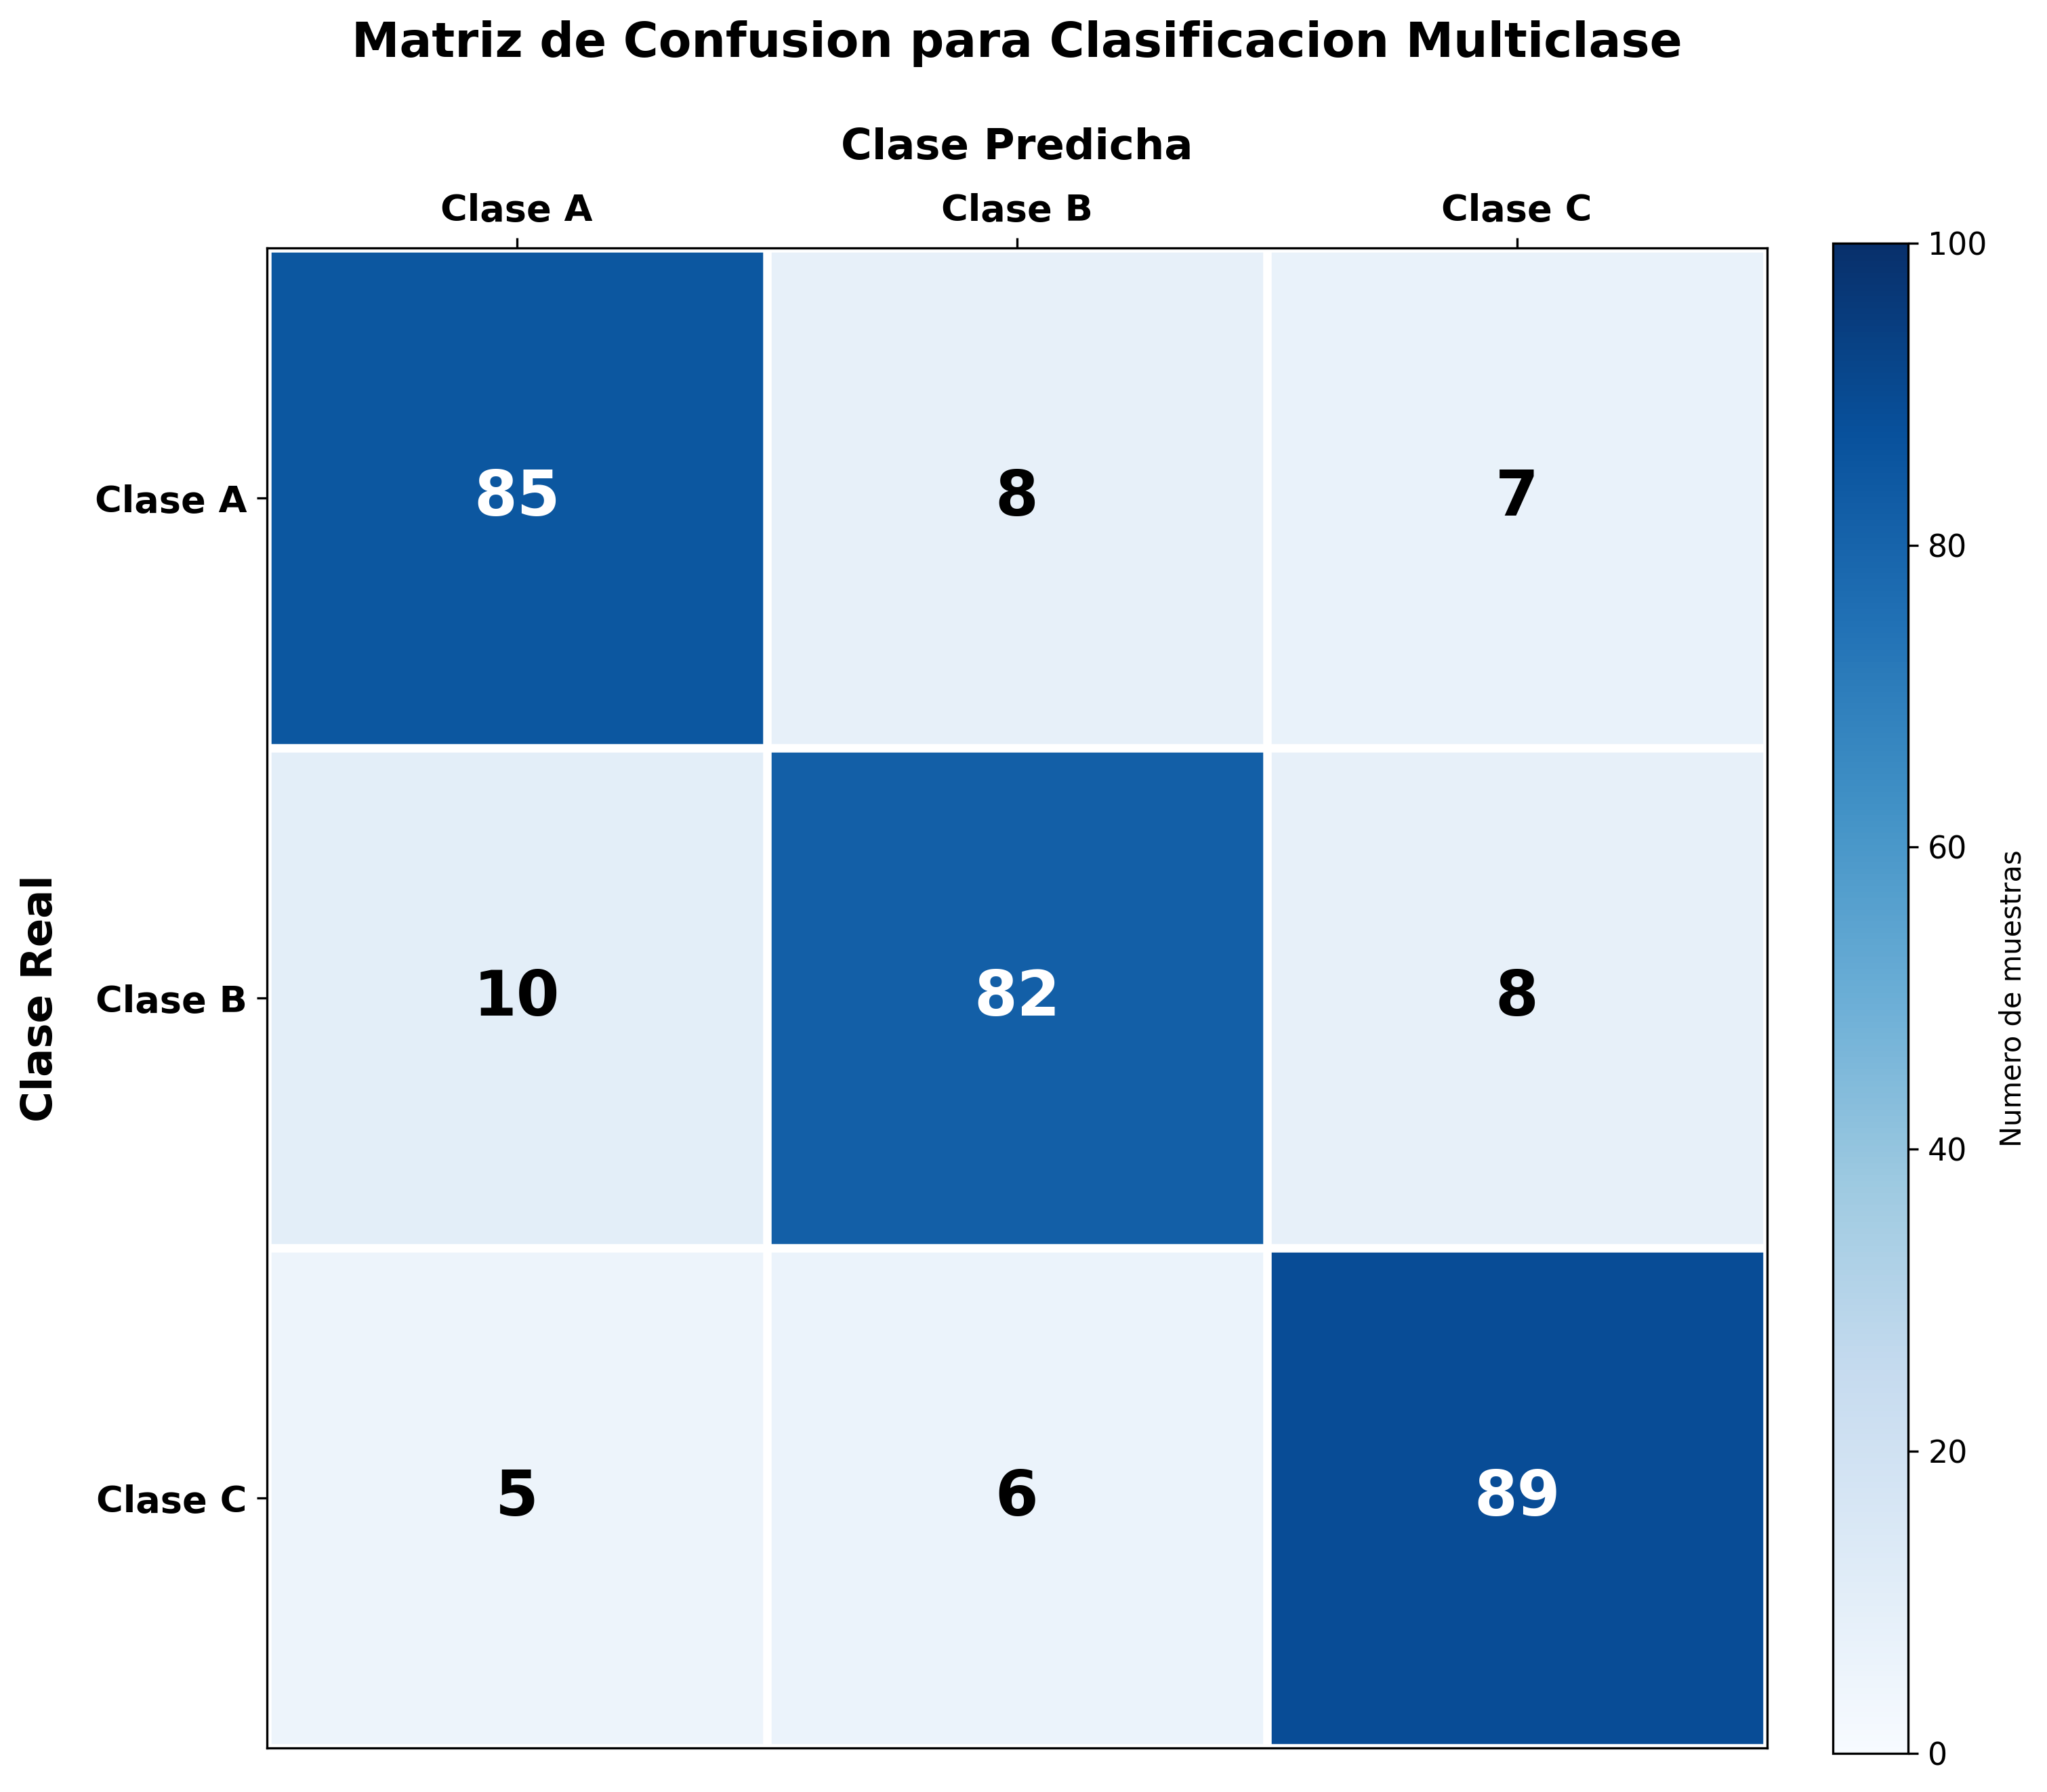
\includegraphics[width=0.65\textwidth]{imagenes/matriz_confusion_ejemplo.png}
\caption{\textit{Matriz de confusión para clasificación multiclase}}
\label{fig:matriz_confusion}
\end{table}

La precisión cuantifica la proporción de predicciones positivas correctas: $\text{Precision} = \text{TP}/(\text{TP} + \text{FP})$. La exhaustividad mide la proporción de casos positivos reales identificados: $\text{Recall} = \text{TP}/(\text{TP} + \text{FN})$. Existe un compromiso inherente entre precisión y recall: aumentar el umbral de decisión incrementa la precisión pero reduce el recall, y viceversa.

\subsubsection{Métricas para calibración espacial}

En sistemas de calibración píxel-milímetro, se emplean métricas de error continuo. El error cuadrático medio (RMSE) cuantifica la magnitud típica de los errores:

\begin{equation}
\text{RMSE} = \sqrt{\frac{1}{N}\sum_{i=1}^{N}(y_i - \hat{y}_i)^2}
\end{equation}

El coeficiente de determinación $R^2$ mide la proporción de varianza explicada por el modelo:

\begin{equation}
R^2 = 1 - \frac{\sum_{i=1}^{N}(y_i - \hat{y}_i)^2}{\sum_{i=1}^{N}(y_i - \bar{y})^2}
\end{equation}

Valores de $R^2$ cercanos a 1 indican excelente ajuste lineal del modelo. Para aplicaciones de agricultura de precisión, se requiere bajo RMSE (típicamente <2mm) y alto $R^2$ (>0.99) para garantizar precisión en el posicionamiento.


\section{Cinemática de Robots Cartesianos}
% Modelado Cinematico


% Espacios Trabajo


% Analisis Trayectorias



\section{Sistemas de Transmisión Mecánica}
% Correa Poleas


% Husillo Tuerca


% Rodamientos Guias



\section{Control de Motores Paso a Paso}

Los motores paso a paso (stepper motors) son actuadores electromecánicos que convierten pulsos eléctricos digitales en movimientos angulares discretos y precisos. A diferencia de los motores de corriente continua convencionales, los motores paso a paso se mueven en incrementos angulares fijos llamados pasos, lo que permite un control de posición en lazo abierto sin necesidad de retroalimentación encoders, aunque estos pueden añadirse para aplicaciones críticas.

\subsubsection{Principio de funcionamiento}

El funcionamiento de un motor paso a paso se basa en la conmutación secuencial de las corrientes en sus bobinas estatóricas, generando campos magnéticos que interactúan con el rotor magnetizado o dentado. Cada pulso de control provoca un movimiento angular discreto del rotor hacia la siguiente posición de equilibrio magnético estable.

El ángulo de paso $\alpha$ define la resolución angular del motor y se expresa como:

\begin{equation}
\alpha = \frac{360^\circ}{N_p}
\end{equation}

donde $N_p$ es el número de pasos por revolución. Los valores típicos de pasos por revolución son 200 ($1.8^\circ$ por paso), 400 ($0.9^\circ$ por paso), aunque mediante técnicas de microstepping se pueden alcanzar resoluciones mucho mayores.

\subsection{Modos de excitación y control}

El modo de excitación define cómo se energizan las bobinas del motor, afectando directamente el torque, la precisión, el consumo de energía y la suavidad del movimiento.

\subsubsection{Excitación de Paso Completo (Full Step)}

\paragraph{Modo de una fase:}

Solo una bobina se energiza a la vez. La secuencia de activación para un motor bipolar de dos fases es:

\begin{table}[ht]
\centering
\begin{tabular}{|c|c|c|}
\hline
\textbf{Paso} & \textbf{Fase A} & \textbf{Fase B} \\
\hline
1 & +I & 0 \\
2 & 0 & +I \\
3 & -I & 0 \\
4 & 0 & -I \\
\hline
\end{tabular}
\caption{Secuencia de excitación Wave Drive}
\end{table}

Características:
\begin{itemize}
    \item Menor consumo de corriente (50\% respecto a dos fases)
    \item Torque reducido (aproximadamente 70\% del torque nominal)
    \item Mayor resonancia a ciertas velocidades
\end{itemize}

\paragraph{Modo de dos fases (Full step):}

Dos bobinas se energizan simultáneamente. La secuencia de activación es:

\begin{table}[ht]
\centering
\begin{tabular}{|c|c|c|}
\hline
\textbf{Paso} & \textbf{Fase A} & \textbf{Fase B} \\
\hline
1 & +I & +I \\
2 & -I & +I \\
3 & -I & -I \\
4 & +I & -I \\
\hline
\end{tabular}
\caption{Secuencia de excitación Full Step}
\end{table}

Características:
\begin{itemize}
    \item Máximo torque disponible (100\% del torque nominal)
    \item Mayor consumo de corriente y generación de calor
    \item Mejor estabilidad posicional
\end{itemize}

\subsubsection{Excitación de medio paso (Half step)}

Alterna entre la energización de una y dos fases, duplicando la resolución del motor. La secuencia combina los modos anteriores:

\begin{table}[ht]
\centering
\begin{tabular}{|c|c|c|}
\hline
\textbf{Paso} & \textbf{Fase A} & \textbf{Fase B} \\
\hline
1 & +I & 0 \\
2 & +I & +I \\
3 & 0 & +I \\
4 & -I & +I \\
5 & -I & 0 \\
6 & -I & -I \\
7 & 0 & -I \\
8 & +I & -I \\
\hline
\end{tabular}
\caption{Secuencia de excitación Half Step}
\end{table}

Para un motor de 200 pasos/rev ($1.8^\circ$), el half stepping proporciona 400 pasos/rev ($0.9^\circ$).

Características:
\begin{itemize}
    \item Resolución duplicada respecto al full step
    \item Torque variable entre pasos (70-100\%)
    \item Mayor suavidad de movimiento
    \item Reducción de resonancia
\end{itemize}

\subsubsection{Microstepping}

El microstepping es una técnica avanzada que subdivide cada paso completo en múltiples micropasos mediante la modulación sinusoidal de las corrientes en las bobinas. Las corrientes en las fases A y B se controlan según:

\begin{equation}
\begin{aligned}
I_A(\theta) &= I_{\max} \cos(\theta) \\
I_B(\theta) &= I_{\max} \sin(\theta)
\end{aligned}
\end{equation}

donde $\theta$ es el ángulo eléctrico deseado e $I_{\max}$ es la corriente máxima nominal.

Para $M$ micropasos por paso completo, el ángulo de micropaso es:

\begin{equation}
\alpha_{\mu} = \frac{\alpha}{M} = \frac{360^\circ}{N_p \cdot M}
\end{equation}

Niveles comunes de microstepping incluyen 1/4, 1/8, 1/16, 1/32, hasta 1/256 pasos.

\paragraph{Ventajas del microstepping:}

\begin{itemize}
    \item Resolución extremadamente alta (hasta 51,200 pasos/rev con 1/256)
    \item Movimiento muy suave y silencioso
    \item Eliminación virtual de resonancia a bajas velocidades
    \item Mejor precisión en posicionamiento fino
\end{itemize}

\paragraph{Limitaciones del microstepping:}

\begin{itemize}
    \item La resolución teórica no garantiza precisión posicional debido a no linealidades
    \item Reducción de torque en micropasos intermedios
    \item Mayor complejidad del driver y procesamiento requerido
    \item Sensibilidad a fricción y errores mecánicos
\end{itemize}

\subsection{Características de desempeño}

\subsubsection{Curvas de torque}

El desempeño de un motor paso a paso se caracteriza principalmente mediante dos curvas de torque:

\paragraph{Torque de retención (Holding torque):}

Es el torque máximo que el motor puede ejercer cuando está energizado pero estacionario. Representa la capacidad de mantener la posición contra cargas externas. Se expresa en N·m o kg·cm y es un parámetro fundamental de selección.

\paragraph{Torque dinámico (Pull-out Torque):}

Es el torque máximo disponible durante el movimiento a una velocidad dada. Esta curva es crítica para determinar si el motor puede acelerar y mantener una carga específica a la velocidad deseada.

La relación entre torque y velocidad se aproxima por:

\begin{equation}
T(\omega) = T_0 \sqrt{1 - \left(\frac{\omega}{\omega_{\max}}\right)^2}
\end{equation}

donde $T_0$ es el torque a velocidad cero (aproximadamente el holding torque), $\omega$ es la velocidad angular, y $\omega_{\max}$ es la velocidad máxima sin carga.

\subsection{Drivers y electrónica de control}

\subsubsection{Tipos de drivers}

\paragraph{Driver unipolar:}

Diseñado para motores unipolares (generalmente con 5 o 6 cables). Utiliza transistores simples para conmutar las corrientes. Ventajas: simplicidad y bajo costo. Desventajas: menor eficiencia y torque (aproximadamente 70\% del equivalente bipolar).

\paragraph{Driver bipolar:}

Para motores bipolares (4 cables). Requiere puentes H para invertir la polaridad de las corrientes. Mayor complejidad pero mejor desempeño. Topologías comunes:

\begin{itemize}
    \item \textbf{L/R Drive}: Control de voltaje simple, genera calor excesivo
    \item \textbf{Chopper Drive}: Modulación PWM de corriente, mayor eficiencia
    \item \textbf{Bipolar con control de corriente}: Regulación precisa mediante sensado de corriente
\end{itemize}

\subsubsection{Interfaces de control}

\paragraph{Step/Direction:}

La interfaz más común. Dos señales digitales:
\begin{itemize}
    \item \textbf{STEP}: Cada pulso produce un paso (o micropaso)
    \item \textbf{DIRECTION}: Define el sentido de rotación (HIGH/LOW)
\end{itemize}

Adicionalmente pueden incluirse señales ENABLE (habilitar motor) y FAULT (indicación de error).

\paragraph{Control por pulsos y sentido:}

Variante donde pulsos en dos líneas diferentes determinan dirección:
\begin{itemize}
    \item Pulsos en CW: Rotación horaria
    \item Pulsos en CCW: Rotación antihoraria
\end{itemize}

\paragraph{Comunicación serial/bus:}

Drivers avanzados incorporan interfaces RS-485, CANbus, o EtherCAT para configuración de parámetros, diagnóstico y control centralizado en sistemas multi-eje.

\subsection{Generación de perfiles de movimiento}

\subsubsection{Perfil trapezoidal}

El perfil de velocidad trapezoidal es el más utilizado por su simplicidad y efectividad. Consta de tres fases:

\begin{enumerate}
    \item \textbf{Aceleración}: Incremento lineal de velocidad desde reposo hasta velocidad objetivo
    \item \textbf{Velocidad constante}: Mantenimiento de la velocidad máxima
    \item \textbf{Deceleración}: Reducción lineal hasta detenerse
\end{enumerate}

Para un desplazamiento angular $\theta_{total}$, con aceleración $\alpha$ y velocidad máxima $\omega_{max}$:

Tiempo de aceleración:
\begin{equation}
t_{acc} = \frac{\omega_{max}}{\alpha}
\end{equation}

Ángulo durante aceleración:
\begin{equation}
\theta_{acc} = \frac{1}{2}\alpha t_{acc}^2 = \frac{\omega_{max}^2}{2\alpha}
\end{equation}

Si el movimiento permite alcanzar $\omega_{max}$:
\begin{equation}
\theta_{cruise} = \theta_{total} - 2\theta_{acc}
\end{equation}

Tiempo total:
\begin{equation}
t_{total} = 2t_{acc} + \frac{\theta_{cruise}}{\omega_{max}}
\end{equation}

Para movimientos cortos donde no se alcanza $\omega_{max}$, la velocidad pico es:
\begin{equation}
\omega_{peak} = \sqrt{\alpha \cdot \theta_{total}}
\end{equation}

\subsection{Análisis de fallos comunes}
\begin{itemize}

    \item{Pérdida de pasos}

\paragraph{Causas:}Torque requerido excede torque disponible, aceleración excesiva, resonancia mecánica, voltaje de alimentación insuficiente a alta velocidad o carga mecánica variable o impactos.

\paragraph{Soluciones:}Aumentar corriente del motor (si térmicamente posible), reducir aceleración máxima, implementar microstepping, incrementar voltaje de alimentación, seleccionar motor de mayor torque o añadir reducción mecánica.

    \item{Resonancia y vibración}

\paragraph{Mitigación:}Cambiar a microstepping (mínimo 1/8), evitar velocidades resonantes en trayectorias, implementar perfiles S-curve, añadir masa o amortiguadores mecánicos, utilizar drivers con anti-resonance features

    \item {Sobrecalentamiento}

\paragraph{Límites térmicos:}La temperatura superficial del motor no debe exceder:
\begin{equation}
T_{surface} < T_{ambient} + \Delta T_{rated}
\end{equation}

Típicamente, $\Delta T_{rated} = 80^\circ$C sobre ambiente.

\paragraph{Soluciones:}Reducir corriente en configuración del driver (sacrificando torque), implementar reducción de corriente en reposo, mejorar ventilación o añadir disipadores, reducir ciclo de trabajo, seleccionar motor de mayor frame size con mejor capacidad térmica.
\end{itemize}

%Los motores paso a paso continúan siendo una solución óptima para aplicaciones que requieren posicionamiento preciso, control digital directo, y operación confiable sin sistemas de retroalimentación complejos. La selección adecuada mediante un proceso sistemático, combinada con configuración apropiada del driver y técnicas de control avanzadas, garantiza un desempeño óptimo y vida útil prolongada del sistema.
% Modos Operacion


% Drivers Electronica



%%%%%%%%%%%%%%%%%%%%%%%%%%%%%%%%%%%%%%%%%%%%%%%%%%%%%%%%%%%%%%%
% CAPÍTULO 3: DESARROLLO DEL SISTEMA
%%%%%%%%%%%%%%%%%%%%%%%%%%%%%%%%%%%%%%%%%%%%%%%%%%%%%%%%%%%%%%%
\chapter{Desarrollo del Sistema}

\section{Arquitectura General del Sistema}
% Diagrama Bloques


% Interaccion Niveles


% Flujo Informacion


% Maquina Estados Global



\section{Modelado y Diseño Mecánico}

\subsection{Especificaciones de Diseño y Restricciones}
\subsubsection{Dimensiones del área de trabajo}

El sistema robótico presenta una configuración cartesiana de dos ejes (XY), con dimensiones de 3~m de ancho por 2~m de alto, diseñado para operar sobre cultivos hidropónicos verticales dispuestos en tubos montados sobre una pared.

\subsubsection{Especificaciones cinemáticas}

Las especificaciones de velocidad, aceleración y resolución de los actuadores se detallan en la Tabla \ref{tab:esp_cinematicas}.

\begin{table}[htbp]
\centering
\begin{tabular}{|l|c|c|}
\hline
\textbf{Parámetro} & \textbf{Eje Horizontal} & \textbf{Eje Vertical} \\ \hline
Velocidad máxima [\(\frac{mm}{s}\)] & 250 & 75 \\ \hline
Velocidad mínima [\(\frac{mm}{s}\)] & 12.5 & 2.5 \\ \hline
Aceleración [\(\frac{mm}{s^2}\)] & 187.5 & 45 \\ \hline
Avance por revolución [\(\frac{mm}{rev}\)] & 40 & 8 \\ \hline
Resolución [\(\frac{pasos}{mm}\)] & 40 & 200 \\ \hline
Micropasos & 8 & 8 \\ \hline
\multicolumn{3}{c}{} \\
\end{tabular}
\caption{Especificaciones cinemáticas de los ejes de movimiento}
\label{tab:esp_cinematicas}
\end{table}

La diferencia en resolución entre ambos ejes responde a los requisitos operativos: el eje horizontal requiere mayor velocidad de desplazamiento con precisión moderada, mientras que el eje vertical necesita mayor precisión de posicionamiento con velocidades menores debido a las operaciones de elevación de carga.

\subsubsection{Cargas del sistema}

Las cargas consideradas en el diseño se distribuyen según su función operativa:\\

Cargas del eje horizontal.\\
\noindent
El motor del eje horizontal debe mover aproximadamente 12~kg, correspondiente a la suma del peso de las varillas verticales, la varilla roscada, los soportes estructurales y el brazo robótico. La carga es soportada principalmente por el perfil superior.

Cargas del eje vertical.\\
\noindent
El motor del eje vertical debe mover la carga correspondiente al peso del brazo robótico y la lechuga (aproximadamente 1.2kg). Además, debe vencer la fricción que se genera entre la tuerca y la varilla roscada.

\subsubsection{Componentes estructurales}

El robot cuenta con tres soportes estructurales principales fabricados mediante impresión 3D:

\begin{itemize}[label=$\bullet$]
    \item \underline{Soporte inferior:} Fijación de las varillas verticales y montaje del motor del eje Z
    \item \underline{Soporte medio:} Sostiene el brazo robótico y la cámara, desplazándose verticalmente mediante la varilla roscada
    \item \underline{Soporte superior:} Acoplamiento cinemático de los dos movimientos perpendiculares (horizontal y vertical), actuando como elemento de unión entre ambos subsistemas
\end{itemize}

El motor del movimiento horizontal estará sostenido por un soporte como el mostrado en la fig. \ref{fig:soporte_motor_pap}
\begin{table}[H]
\centering
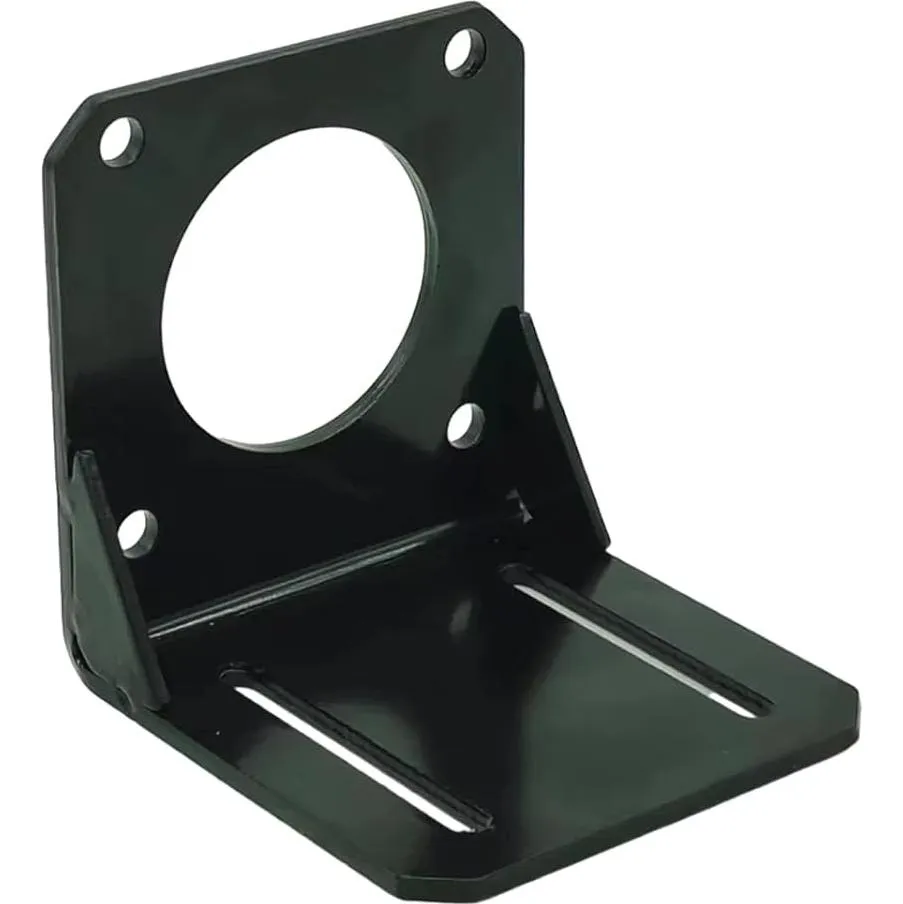
\includegraphics[width=0.25\textwidth]{img/soporte_motor_pap.png}
\caption{\textit{Referencia de oporte para motor pap.}}
\label{fig:soporte_motor_pap}
\end{table}
El perfil superior se une a un caño estructural en cada extremo utilizando soportes tipo L. Mientras que el perfil lateral que brinda rigidez, se atornilla también a un tramo de caño estructural en cada extremo. Las orientaciones de los caños estructurales de soporte se puede observar en la fig. \ref{fig:ClaudioReal_simplificado}

\subsection{Análisis Cinemático del Sistema}
% Grados Libertad


% Ecuaciones Movimiento


% Espacio Trabajo



\subsection{Diseño Estructural}
% Seleccion Materiales


% Calculos Resistencia


% Estructura Soporte



\subsection{Sistema de Movimiento Horizontal}
% Dimensionamiento Correa


% Seleccion Poleas


% Calculo Cargas Horizontal



\subsection{Sistema de Movimiento Vertical}
% Analisis Husillo


% Calculo Torque


% Seleccion Guias



\subsection{Brazo Robótico}
Se cuenta con un brazo de dos grados de libertad controlables para el posicionamiento del efector final que es de tipo pinza.

\subsubsection{Descripción del Sistema}

El brazo robótico consiste en una configuración planar de dos eslabones articulados mediante juntas rotacionales, con un efector final tipo gripper de pinza. Este sistema posee dos grados de libertad en el plano, definidos por los ángulos de rotación $\theta_1$ y $\theta_2$ de cada articulación.

\subsubsection{Parámetros Geométricos}

\begin{itemize}
    \item $L_1$: Longitud del primer eslabón (eslabón proximal)
    \item $L_2$: Longitud del segundo eslabón (eslabón distal)
    \item $\theta_1$: Ángulo de la primera articulación (base)
    \item $\theta_2$: Ángulo de la segunda articulación (codo)
\end{itemize}

\subsubsection{Cinemática Directa}

La cinemática directa establece la relación entre las coordenadas articulares $(\theta_1, \theta_2)$ y la posición del efector final $(x, y)$ en el plano.

La posición del efector final se calcula mediante:

\begin{align}
    x &= L_1 \cdot \cos(\theta_1) + L_2 \cdot \cos(\theta_1 + \theta_2) \\
    y &= L_1 \cdot \sin(\theta_1) + L_2 \cdot \sin(\theta_1 + \theta_2)
\end{align}

La orientación del efector final está dada por:

\begin{equation}
    \phi = \theta_1 + \theta_2
\end{equation}

\subsubsection{Cinemática Inversa}

La cinemática inversa determina los ángulos articulares necesarios para alcanzar una posición deseada $(x_d, y_d)$. Este problema presenta dos soluciones posibles (configuración de codo arriba y codo abajo).

Primero se calcula el ángulo $\theta_2$:

\begin{equation}
    \cos(\theta_2) = \frac{x_d^2 + y_d^2 - L_1^2 - L_2^2}{2 \cdot L_1 \cdot L_2}
\end{equation}

\begin{equation}
    \theta_2 = \pm \arccos\left(\frac{x_d^2 + y_d^2 - L_1^2 - L_2^2}{2 \cdot L_1 \cdot L_2}\right)
\end{equation}

Luego se determina $\theta_1$:

\begin{equation}
    \theta_1 = \arctan2(y_d, x_d) - \arctan2(L_2 \cdot \sin(\theta_2), L_1 + L_2 \cdot \cos(\theta_2))
\end{equation}

\subsubsection{Espacio de Trabajo}

El espacio de trabajo accesible para el efector final es un anillo circular con:

\begin{itemize}
    \item Radio máximo: $R_{max} = L_1 + L_2$ (brazo completamente extendido)
    \item Radio mínimo: $R_{min} = |L_1 - L_2|$ (brazo completamente plegado)
\end{itemize}

\subsubsection{Jacobiano}

El Jacobiano relaciona las velocidades articulares con las velocidades del efector final:

\begin{equation}
    \begin{bmatrix}
        \dot{x} \\
        \dot{y}
    \end{bmatrix}
    =
    \begin{bmatrix}
        J_{11} & J_{12} \\
        J_{21} & J_{22}
    \end{bmatrix}
    \begin{bmatrix}
        \dot{\theta}_1 \\
        \dot{\theta}_2
    \end{bmatrix}
\end{equation}

Donde:

\begin{align}
    J_{11} &= -L_1 \cdot \sin(\theta_1) - L_2 \cdot \sin(\theta_1 + \theta_2) \\
    J_{12} &= -L_2 \cdot \sin(\theta_1 + \theta_2) \\
    J_{21} &= L_1 \cdot \cos(\theta_1) + L_2 \cdot \cos(\theta_1 + \theta_2) \\
    J_{22} &= L_2 \cdot \cos(\theta_1 + \theta_2)
\end{align}

\subsubsection{Gripper Tipo Pinza}

El gripper se ubica en el extremo del segundo eslabón y posee un grado de libertad adicional (no considerado en los 2 GDL principales) para la apertura/cierre de las mandíbulas, controlado por el parámetro $d$ (distancia entre mandíbulas).

\subsubsection{Singularidades}

El sistema presenta singularidades cuando el determinante del Jacobiano es cero:

\begin{equation}
    \det(J) = L_1 \cdot L_2 \cdot \sin(\theta_2) = 0
\end{equation}

Esto ocurre cuando \(\theta_2 = 0^\circ \) o \(\theta_2 = 180^\circ\), es decir, cuando el brazo está completamente extendido o plegado.


% Cinematica Brazo


\section{Dimensionamiento de Servomotores}

El brazo robótico diseñado para la cosecha de lechugas cuenta con dos grados de libertad, equivalentes a una articulación de hombro y una de codo. El sistema debe ser capaz de extenderse horizontalmente para alcanzar y tomar la carga (lechuga), para luego contraerse y transportarla de manera eficiente.

\subsection{Parámetros del Sistema}

Los parámetros físicos y operacionales del brazo robótico se detallan en la Tabla \ref{tab:parametros_brazo}.

\begin{table}[htbp]
\centering
\caption{Parámetros del brazo robótico}
\label{tab:parametros_brazo}
\begin{tabular}{lcc}
\hline
\textbf{Parámetro} & \textbf{Valor} & \textbf{Unidad} \\
\hline
Longitud eslabón 1 ($L_1$) & 16 & cm \\
Longitud eslabón 2 ($L_2$) & 12.5 & cm \\
Masa del brazo ($m_{brazo}$) & 300 & g \\
Masa de la carga ($m_{carga}$) & 400 & g \\
Velocidad angular máxima ($\omega_{\max}$) & 45 & $^{\circ}$/s \\
Tiempo de aceleración ($t_{ac}$) & 0.5 & s \\
\hline
\end{tabular}
\end{table}

El movimiento del brazo involucra tanto desplazamiento horizontal como elevación vertical, partiendo desde una posición horizontal hasta una posición elevada para transportar la carga. Por lo tanto, el análisis debe considerar tanto el torque dinámico necesario para acelerar las masas como el torque estático requerido para sostener el brazo contra la gravedad.

\subsection{Dimensionamiento del Motor del Codo}

El servomotor del codo es responsable del movimiento de la carga ubicada en el extremo del segundo eslabón y debe soportarla contra la gravedad.

\subsubsection{Torque Estático (Gravitacional)}

En la posición horizontal, el torque necesario para sostener la carga es:

\begin{equation}
\tau_{est,codo} = m_{carga} \cdot g \cdot \frac{L_2}{2}
\end{equation}

donde se considera el centro de masa de la carga en el punto medio del eslabón. Sustituyendo valores:

\begin{equation}
\tau_{est,codo} = 0.4 \, \text{kg} \cdot 9.81 \, \text{m/s}^2 \cdot 0.0625 \, \text{m} = 0.245 \, \text{N} \cdot \text{m}
\end{equation}

\subsubsection{Momento de Inercia}

El momento de inercia de la carga con respecto al eje del codo se calcula como:

\begin{equation}
I_{codo} = m_{carga} \cdot L_2^2
\end{equation}

Sustituyendo valores:

\begin{equation}
I_{codo} = 0.4 \, \text{kg} \cdot (0.125 \, \text{m})^2 = 6.25 \times 10^{-3} \, \text{kg} \cdot \text{m}^2
\end{equation}

\subsubsection{Aceleración Angular}

La aceleración angular necesaria para alcanzar la velocidad máxima en el tiempo especificado es:

\begin{equation}
\alpha = \frac{\omega_{max}}{t_{ac}} = \frac{0.785 \, \text{rad/s}}{0.5 \, \text{s}} = 1.57 \, \text{rad/s}^2
\end{equation}

donde $\omega_{max} = 45° \cdot \frac{\pi}{180°} = 0.785 \, \text{rad/s}$.

\subsubsection{Torque Dinámico}

El torque dinámico requerido se obtiene mediante:

\begin{equation}
\tau_{din,codo} = I_{codo} \cdot \alpha = 6.25 \times 10^{-3} \cdot 1.57 = 9.8 \times 10^{-3} \, \text{N} \cdot \text{m}
\end{equation}

\subsubsection{Torque Total}

El torque total necesario suma los componentes estático y dinámico:

\begin{equation}
\tau_{codo,total} = \tau_{est,codo} + \tau_{din,codo} = 0.245 + 0.0098 = 0.255 \, \text{N} \cdot \text{m}
\end{equation}

Aplicando un factor de seguridad de 1.5 para considerar fricciones, pérdidas y variaciones en la carga:

\begin{equation}
\tau_{codo} = 1.5 \cdot \tau_{codo,total} = 0.38 \, \text{N} \cdot \text{m} \approx 39 \, \text{kg} \cdot \text{cm}
\end{equation}

\subsection{Dimensionamiento del Motor del Hombro}

El servomotor del hombro debe proporcionar el torque necesario para mover el brazo completo, soportar su peso y el de la carga contra la gravedad, especialmente en la posición horizontal.

\subsubsection{Torque Estático (Gravitacional)}

En la posición horizontal (peor caso), el torque gravitacional resulta de la suma de los momentos de todas las masas:

\begin{equation}
\tau_{est,hombro} = m_{brazo} \cdot g \cdot \frac{L_1}{2} + m_{carga} \cdot g \cdot L_{total}
\end{equation}

Sustituyendo valores:

\begin{equation}
\tau_{est,hombro} = 0.3 \cdot 9.81 \cdot 0.08 + 0.4 \cdot 9.81 \cdot 0.285 = 0.235 + 1.118 = 1.353 \, \text{N} \cdot \text{m}
\end{equation}

\subsubsection{Momento de Inercia Total}

El momento de inercia total respecto al eje del hombro se compone de tres contribuciones:

\textbf{a) Inercia del primer eslabón:} Considerando una distribución uniforme de masa:

\begin{equation}
I_{eslabón1} = \frac{m_{brazo}}{2} \cdot \frac{L_1^2}{3} = 0.15 \cdot \frac{(0.16)^2}{3} = 1.28 \times 10^{-3} \, \text{kg} \cdot \text{m}^2
\end{equation}

\textbf{b) Inercia del segundo eslabón:} Aproximando su masa concentrada en el codo:

\begin{equation}
I_{eslabón2} = \frac{m_{brazo}}{2} \cdot L_1^2 = 0.15 \cdot (0.16)^2 = 3.84 * 10^{-3} \, \text{kg} \cdot \text{m}^2
\end{equation}

\textbf{c) Inercia de la carga:} Con el brazo completamente extendido ($L_{total} = L_1 + L_2 = 0.285$ m):

\begin{equation}
I_{carga,hombro} = m_{carga} \cdot L_{total}^2 = 0.4 \cdot (0.285)^2 = 3.25 \times 10^{-2} \, \text{kg} \cdot \text{m}^2
\end{equation}

El momento de inercia total resulta:

\begin{equation}
I_{hombro} = I_{eslabón1} + I_{eslabón2} + I_{carga,hombro} = 3.76 \times 10^{-2} \, \text{kg} \cdot \text{m}^2
\end{equation}

\subsubsection{Torque Dinámico}

Utilizando la misma aceleración angular calculada anteriormente:

\begin{equation}
\tau_{din,hombro} = I_{hombro} \cdot \alpha = 3.76 \times 10^{-2} \cdot 1.57 = 5.9 \times 10^{-2} \, \text{N} \cdot \text{m}
\end{equation}

\subsubsection{Torque Total}

El torque total combina los componentes estático y dinámico:

\begin{equation}
\tau_{hombro,total} = \tau_{est,hombro} + \tau_{din,hombro} = 1.353 + 0.059 = 1.412 \, \text{N} \cdot \text{m}
\end{equation}

Con factor de seguridad de 1.5:

\begin{equation}
\tau_{hombro} = 1.5 \cdot \tau_{hombro,total} = 2.12 \, \text{N} \cdot \text{m} \approx 216 \, \text{kg} \cdot \text{cm}
\end{equation}

\subsection{Resultados y Selección de Servomotores}

La Tabla \ref{tab:resultados_torque} resume los torques mínimos requeridos para cada articulación.

\begin{table}[h]
\centering
\caption{Torques mínimos requeridos}
\label{tab:resultados_torque}
\begin{tabular}{lccc}
\hline
\textbf{Articulación} & \textbf{Torque Estático} & \textbf{Torque Total} & \textbf{Con Seguridad} \\
 & \textbf{(kg·cm)} & \textbf{(kg·cm)} & \textbf{(kg·cm)} \\
\hline
Codo & 25 & 26 & 39 \\
Hombro & 138 & 144 & 216 \\
\hline
\end{tabular}
\end{table}

En base a estos requerimientos, se proponen las siguientes opciones de servomotores:

\textbf{Motor del Codo (39 kg·cm):}
\begin{itemize}
    \item Dynamixel MX-28: 24 kg·cm @ 12V (requiere reducción 2:1)
    \item Dynamixel MX-64: 60 kg·cm @ 12V (opción recomendada)
    \item Servo industrial con reductor: torque nominal > 40 kg·cm
\end{itemize}

\textbf{Motor del Hombro (216 kg·cm):}
\begin{itemize}
    \item Dynamixel MX-106: 84 kg·cm @ 12V (requiere reducción 3:1)
    \item Servomotor industrial Nema 23 con reductor planetario
    \item Sistema de poleas/engranajes con motor de menor torque (relación 4:1 o 5:1)
\end{itemize}

Dada la magnitud del torque requerido, especialmente en el hombro, se recomienda implementar un sistema de reducción mecánica mediante poleas dentadas o reductores planetarios, lo que permitirá utilizar motores más económicos y con mejor respuesta dinámica.

\subsection{Consideraciones Adicionales}

El análisis presentado considera el peor caso operacional, con el brazo en posición horizontal donde el torque gravitacional es máximo. Durante la operación:

\begin{itemize}
    \item \textbf{Posición inicial (horizontal):} Requiere el máximo torque para sostener y mover la carga.
    \item \textbf{Posición elevada:} Al contraer el brazo verticalmente, el momento gravitacional disminuye significativamente, ya que el brazo de palanca se reduce al elevarse.
    \item \textbf{Estrategia de movimiento:} Se recomienda una trayectoria que minimice el tiempo en posición horizontal, elevando el brazo lo más rápido posible después de tomar la carga.
\end{itemize}

El componente de torque estático representa aproximadamente el 96\% del torque total en el hombro y el 94\% en el codo, lo que indica que el sistema está dominado por cargas gravitacionales más que por requisitos dinámicos. Esto sugiere que velocidades de movimiento moderadas son apropiadas para esta aplicación.

Se recomienda el uso de servomotores con retroalimentación de posición y corriente para implementar control de torque, permitiendo detectar colisiones durante el agarre y optimizar el consumo energético ajustando el torque según la posición del brazo.

\subsection{Modelado CAD y Fabricación}
% Diseno Piezas 3D


% Tecnologia Impresion


% Tolerancias Ajustes



\section{Sistema de Control de Bajo Nivel (Nivel Regulatorio)}

\subsection{Arquitectura del Nivel Regulatorio}
El nivel regulatorio constituye el sistema de control en tiempo real del robot, gestionando directamente actuadores y sensores mediante ejecución de comandos recibidos desde el nivel supervisor.

El firmware se estructura en tres capas jerárquicas que separan responsabilidades según nivel de abstracción, como se muestra en la Figura \ref{fig:arquitectura_regulatorio}:

\begin{itemize}[label=$\bullet$]
\item \textbf{Capa de controladores de hardware (drivers):} Interactúa directamente con periféricos del microcontrolador mediante registros y temporizadores
\item \textbf{Capa de control de movimiento:} Implementa generación de trayectorias mediante perfiles de velocidad y coordinación de ejes
\item \textbf{Capa de aplicación:} Proporciona interfaz de alto nivel para comandos del sistema supervisor mediante protocolo UART
\end{itemize}

\begin{figure}[H]
    \centering
    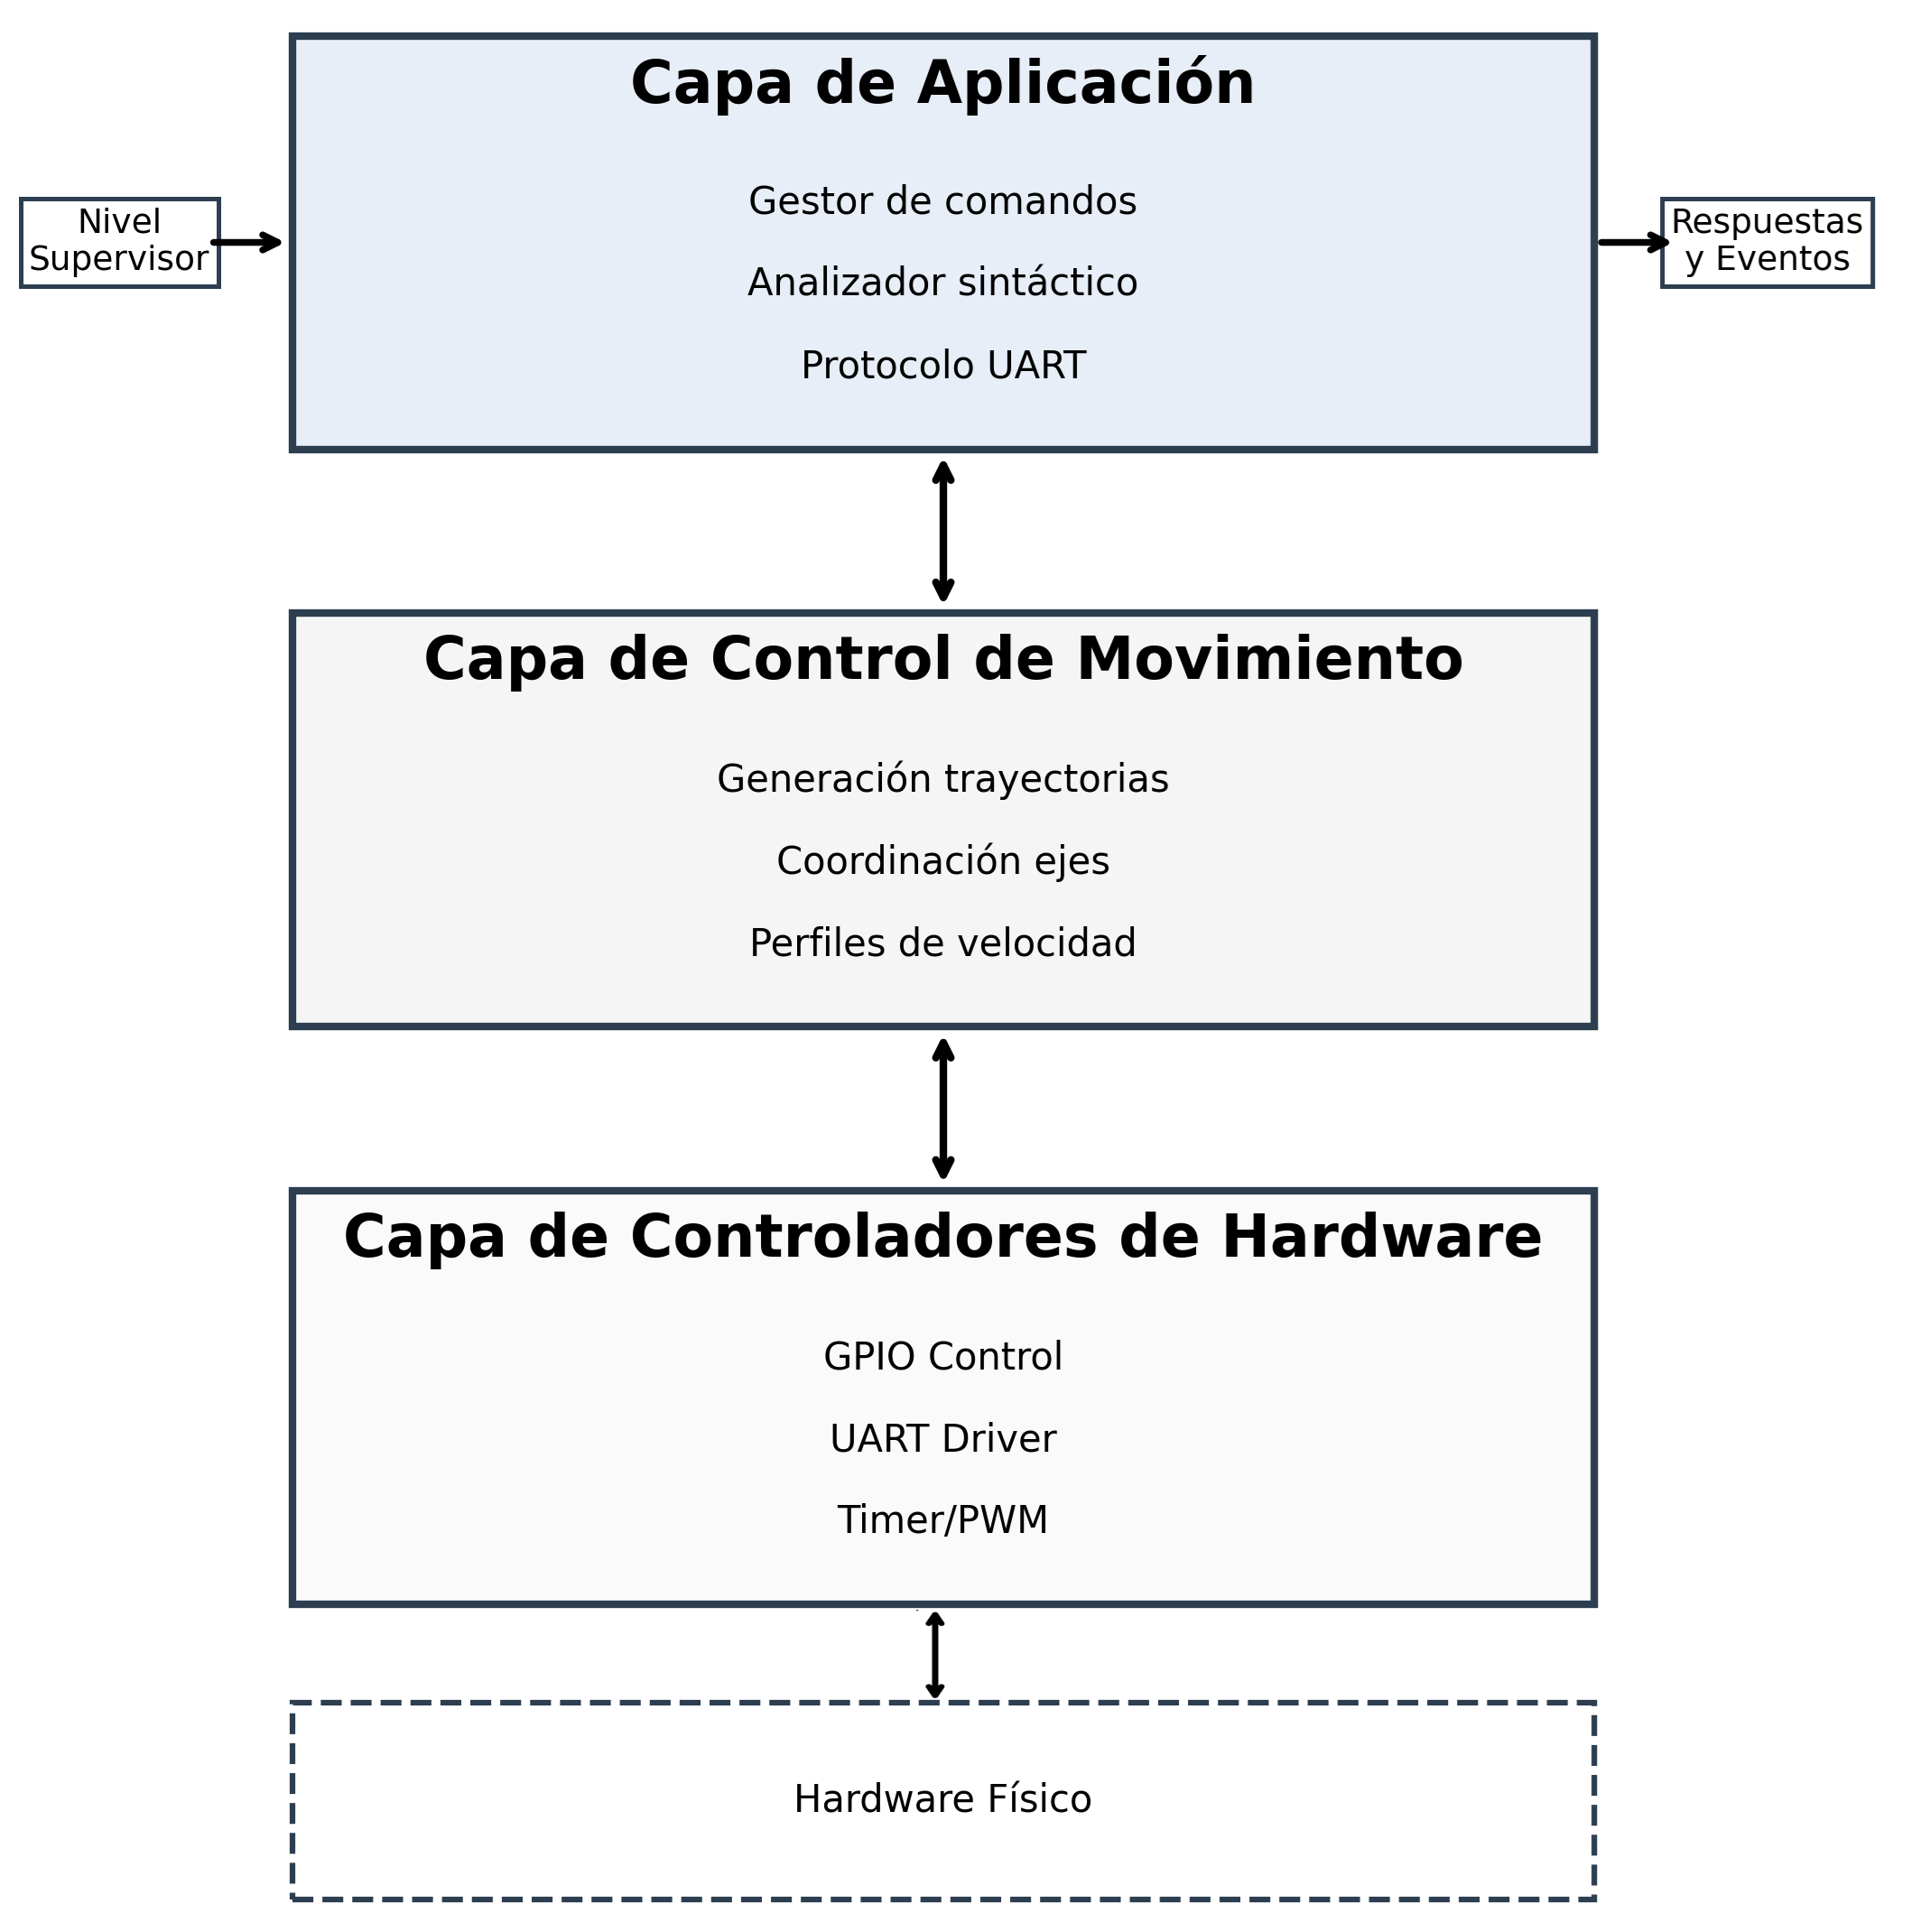
\includegraphics[width=0.7\textwidth]{imagenes/arquitectura_regulatorio_capas.png}
    \caption{\textit{Arquitectura en capas del firmware del nivel regulatorio}}
    \label{fig:arquitectura_regulatorio}
\end{figure}


\subsection{Hardware de Control - Arduino Mega 2560}
Los requerimientos principales que debe cumplir el controlador incluyen la generación de pulsos de alta frecuencia para motores paso a paso operando hasta 10,000 pasos/s, la disponibilidad de múltiples temporizadores por hardware para controlar dos ejes de motores paso a paso y dos servomotores de forma concurrente, señales de nivel lógico de 5V compatibles directamente con los drivers TB6600 y servomotores utilizados, un mínimo de 16 pines GPIO para comandar steppers (STEP, DIR, ENABLE para dos ejes), servomotores, finales de carrera y actuador de agarre, comunicación UART por hardware a 115200 baudios sin bloquear el loop de control, y memoria suficiente para almacenar el firmware (aproximadamente 15KB de Flash) y mantener estructuras de datos en tiempo de ejecución (1.2KB de RAM).

Teniendo en cuenta los puntos anteriores se selecciono un Arduino Mega 2560 como plataforma de control por satisfacer todos los requerimientos del sistema y proveer recursos adicionales para futuras expansiones. Este microcontrolador está basado en el ATmega2560 de 8 bits de Microchip (anteriormente Atmel), que opera a 16MHz con arquitectura RISC AVR, lo que resulta suficiente para ejecutar loops de control a frecuencias superiores a 10kHz con latencias predecibles, cumpliendo ampliamente los requisitos de temporización del sistema.

En términos de memoria, cuenta con 256KB de memoria Flash para almacenar el programa (el firmware actual utiliza aproximadamente 15KB, representando solo un 6\% de uso), 8KB de SRAM para variables y estructuras de datos en tiempo de ejecución (uso actual de 1.2KB, equivalente al 15\%), y 4KB de EEPROM para almacenamiento persistente de parámetros de configuración como velocidades máximas, aceleraciones y límites de recorrido.

Los recursos de hardware incluyen 6 temporizadores (cuatro de 16 bits: Timer1, Timer3, Timer4 y Timer5; dos de 8 bits: Timer0 y Timer2), 54 pines digitales de entrada/salida configurables, 16 entradas analógicas con conversores ADC de 10 bits, 4 UARTs por hardware independientes y 15 canales de PWM por hardware. Esta abundancia de recursos permite asignar un temporizador dedicado para la generación de pulsos de steppers (Timer1) y dos temporizadores independientes para los servomotores (Timer4 y Timer5), evitando conflictos de recursos.

Un aspecto crítico de la selección fue la compatibilidad de nivel lógico. El ATmega2560 opera a 5V, mientras que alternativas modernas como los microcontroladores STM32 de 32 bits (basados en ARM Cortex-M) o ESP32 operan a 3.3V. Los drivers de motores paso a paso TB6600 y servomotores seleccionados requieren señales de entrada de 5V. El uso de un microcontrolador de 3.3V requeriría circuitería adicional de level shifting (conversores de nivel lógico bidireccionales), incrementando la complejidad del diseño, el costo de componentes, y potencialmente introduciendo retardos adicionales.

La selección del Arduino Mega 2560 representa un equilibrio óptimo entre capacidad de procesamiento, recursos de hardware, compatibilidad eléctrica directa con los actuadores, precio y facilidad de desarrollo.
% Este archivo fue vaciado. La distribución de pines del Arduino se movió a la sección de selección de componentes.


\subsection{Selección y Dimensionamiento de Actuadores}
% Motores Paso Paso


% Drivers Tb6600


% Servomotores



\subsection{Sensores de Seguridad}
% Finales Carrera


% Sistema Seguridad



\subsection{Control de Movimiento}
\subsubsection{Perfiles de Velocidad para Control de Movimiento}

El sistema implementa perfiles de velocidad trapezoidales con aceleraciones fijas, garantizando comportamiento predecible independientemente de la distancia del movimiento. Las distancias de aceleración y desaceleración permanecen constantes, variando únicamente la longitud de la zona de crucero.

Para movimientos largos (superiores a 25mm), el perfil se compone de las fases mostradas en la Tabla \ref{tab:perfil_trapezoidal}. Esta estrategia asegura que las aceleraciones sean idénticas para todos los movimientos, proporcionando comportamiento mecánico consistente. Por ejemplo, un movimiento de 25mm tiene 12.5mm de aceleración/desaceleración y 12.5mm de crucero, mientras que un movimiento de 250mm mantiene los mismos 12.5mm de aceleración/desaceleración pero dispone de 237.5mm de crucero.

\begin{table}[H]
\centering
\small
\begin{tabular}{|l|c|c|c|c|}
\hline
\textbf{Fase} & \textbf{Distancia} & \textbf{$v_i$} & \textbf{$v_f$} & \textbf{Aceleración} \\
\hline
1. Arranque & Instant. & 0 & 0.05 & - \\
\hline
2. Acel. suave & 5 mm & 0.05 & 0.10 & 0.05 m/s² \\
\hline
3. Acel. fuerte & 7.5 mm & 0.10 & 0.375 (H) / 0.30 (V) & 0.37 / 0.27 m/s² \\
\hline
4. Crucero & Variable & 0.375 / 0.30 & 0.375 / 0.30 & 0 \\
\hline
5. Decel. fuerte & 7.5 mm & 0.375 / 0.30 & 0.10 & -0.37 / -0.27 m/s² \\
\hline
6. Decel. suave & 5 mm & 0.10 & 0.05 & -0.05 m/s² \\
\hline
7. Detención & Instant. & 0.05 & 0 & - \\
\hline
\end{tabular}
\caption{Fases del perfil trapezoidal de velocidad con aceleraciones fijas. Velocidades en m/s, H: horizontal, V: vertical}
\label{tab:perfil_trapezoidal}
\end{table}

\begin{figure}[H]
    \centering
    % TODO: Insertar gráfico comparativo mostrando mismo perfil de aceleración para diferentes distancias
    % Mostrar: dos movimientos (25mm vs 250mm) con mismas rampas de accel/decel pero diferente zona crucero
    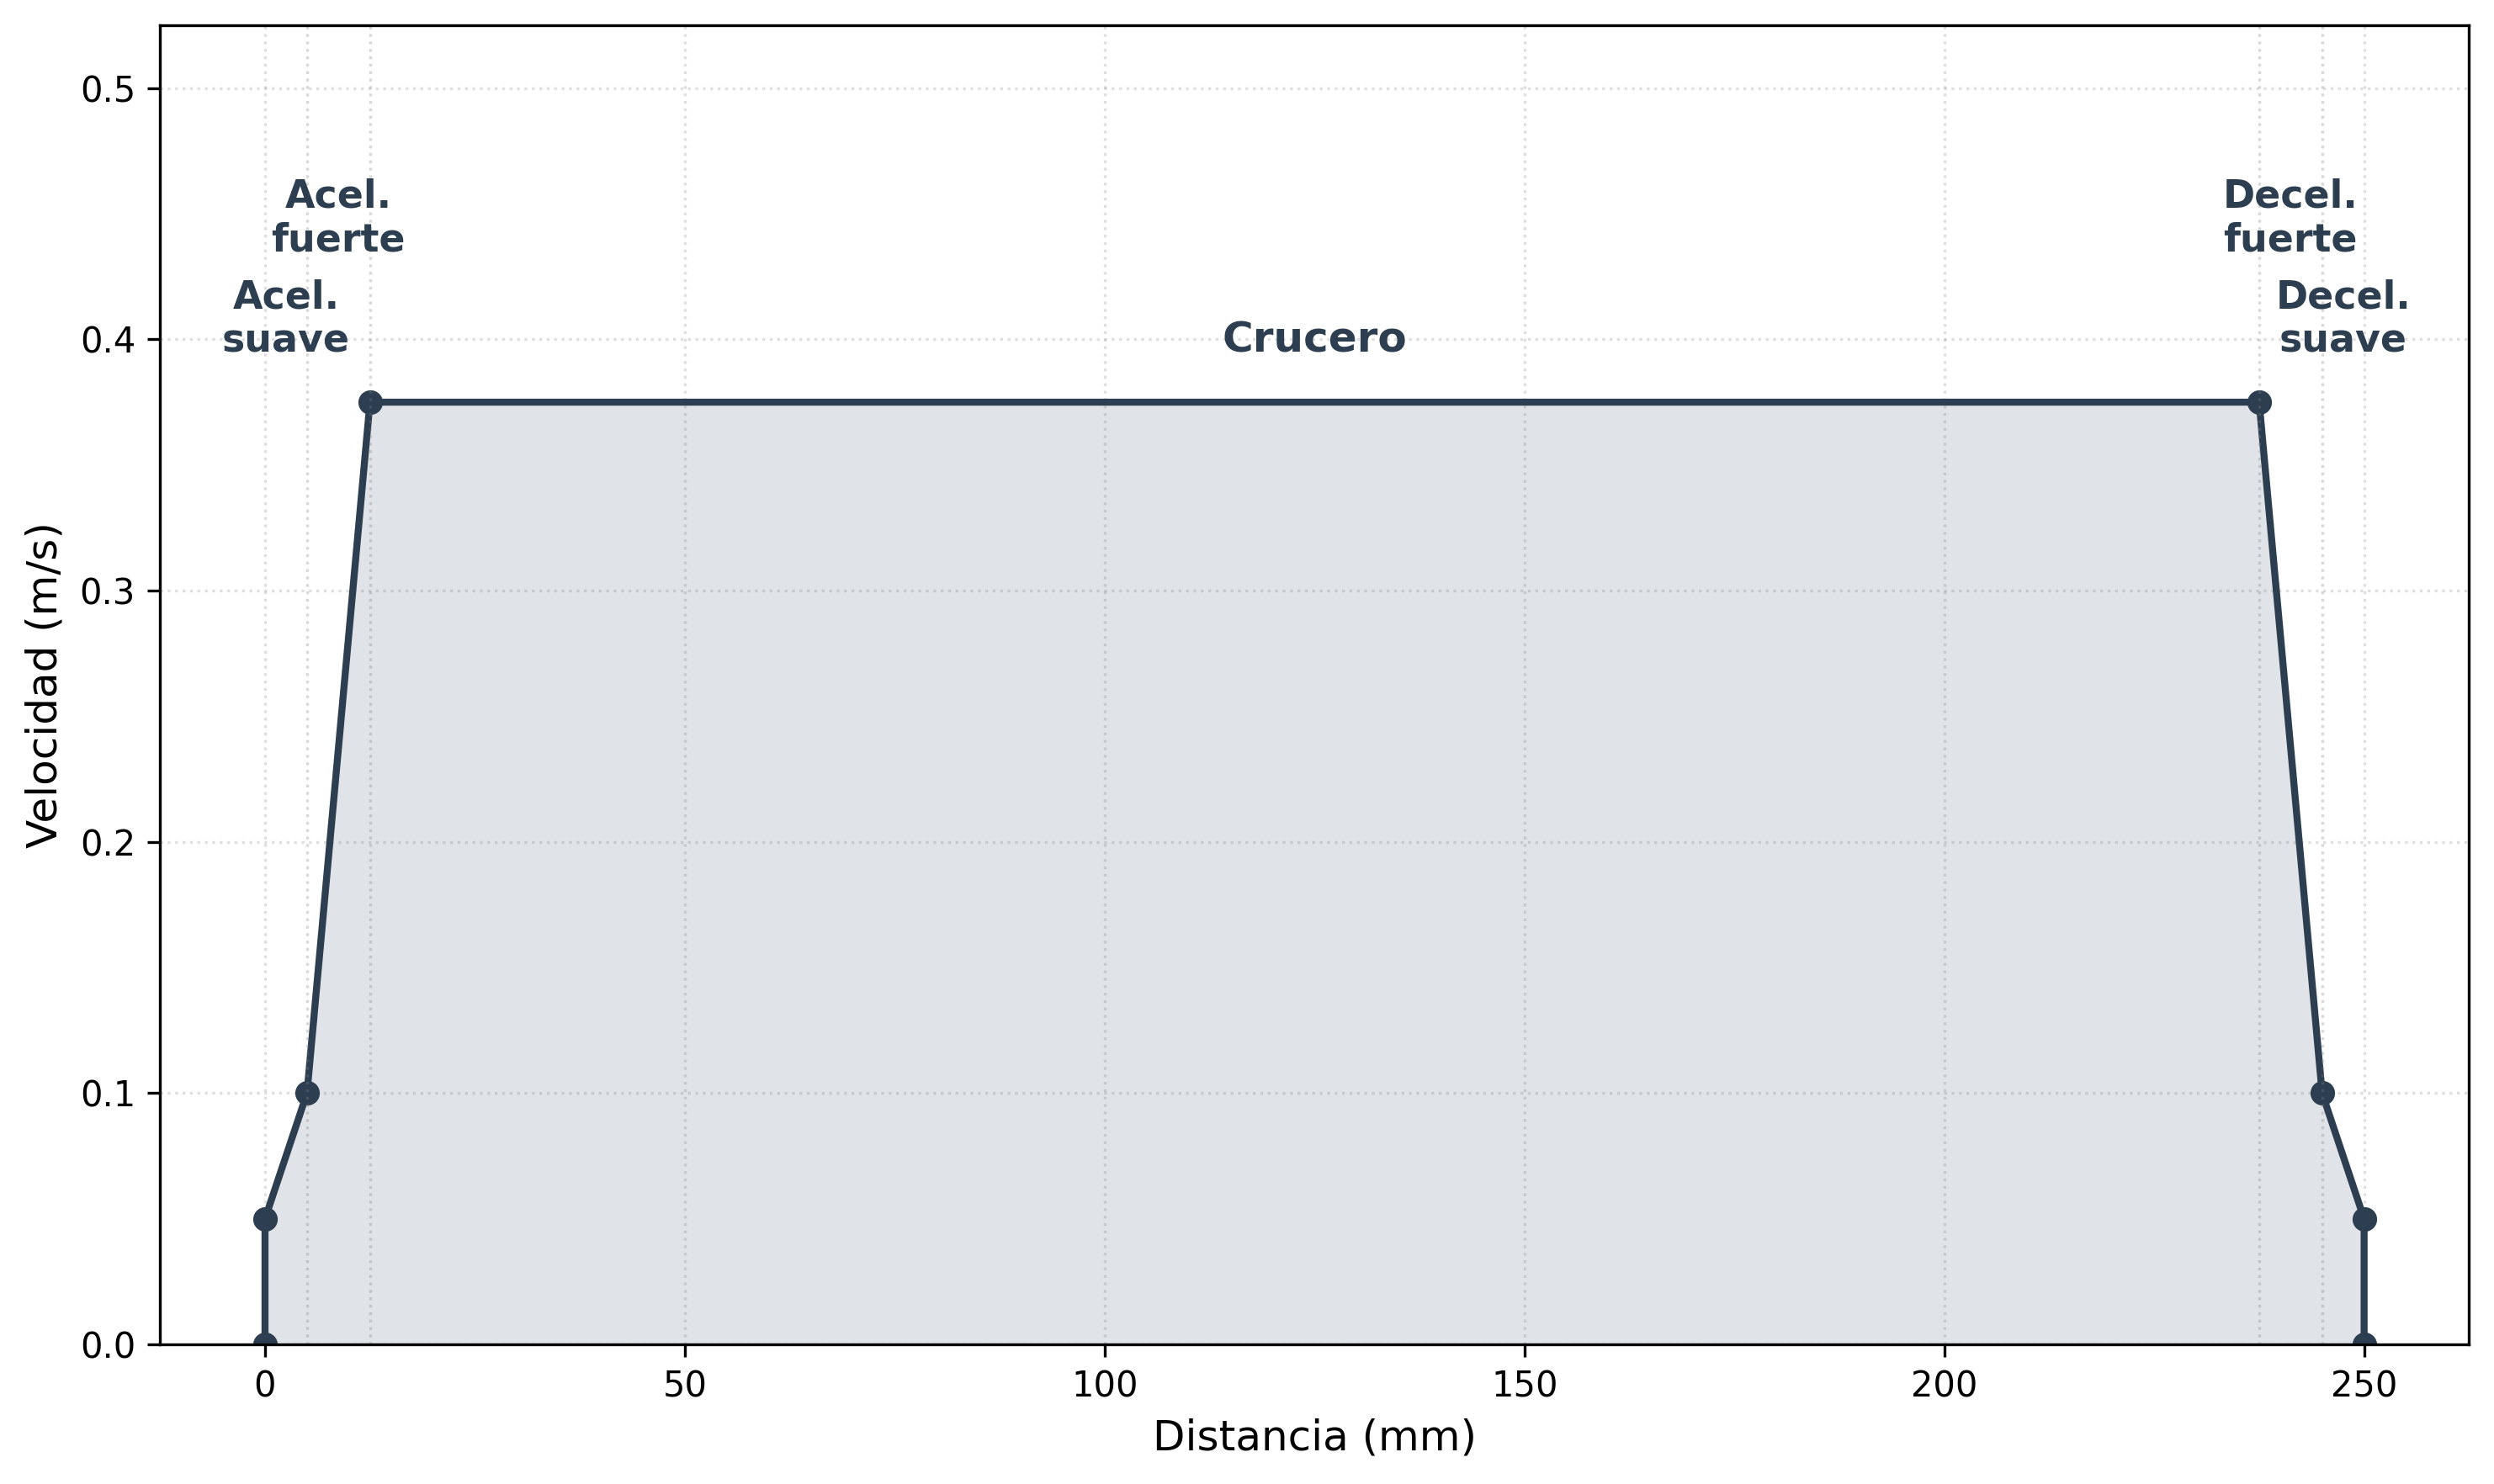
\includegraphics[width=0.7\textwidth]{imagenes/perfil_trapezoidal_velocidad.png}
    \caption{Perfil trapezoidal con aceleraciones fijas. Las zonas de aceleración y desaceleración mantienen longitud constante (12.5mm cada una), mientras que la zona de crucero se ajusta según la distancia total}
    \label{fig:perfil_trapezoidal}
\end{figure}

Cuando la distancia total es menor que 25mm (suma de las zonas de aceleración y desaceleración), el perfil se convierte en triangular. El sistema mantiene las mismas aceleraciones de la Tabla \ref{tab:perfil_trapezoidal}, pero calcula el punto medio del movimiento donde debe iniciar la desaceleración para alcanzar exactamente la posición final. En este caso, la velocidad máxima alcanzada es menor que la velocidad de crucero nominal, ya que el motor comienza a frenar antes de alcanzarla. Por ejemplo, un movimiento de 10mm acelera durante 5mm hasta alcanzar aproximadamente 0.15 m/s, y luego desacelera durante los siguientes 5mm hasta detenerse (Figura \ref{fig:perfil_comparacion}).

Para movimientos muy cortos (menos de 2.5mm), el sistema reduce la velocidad máxima permitida a 0.10 m/s para mantener precisión en el posicionamiento final, típico en operaciones de ajuste fino.

\begin{figure}[H]
    \centering
    % TODO: Insertar gráfico comparativo: perfil trapezoidal vs triangular
    % Mostrar: movimiento largo con zona crucero vs movimiento corto sin zona crucero (triangular)
    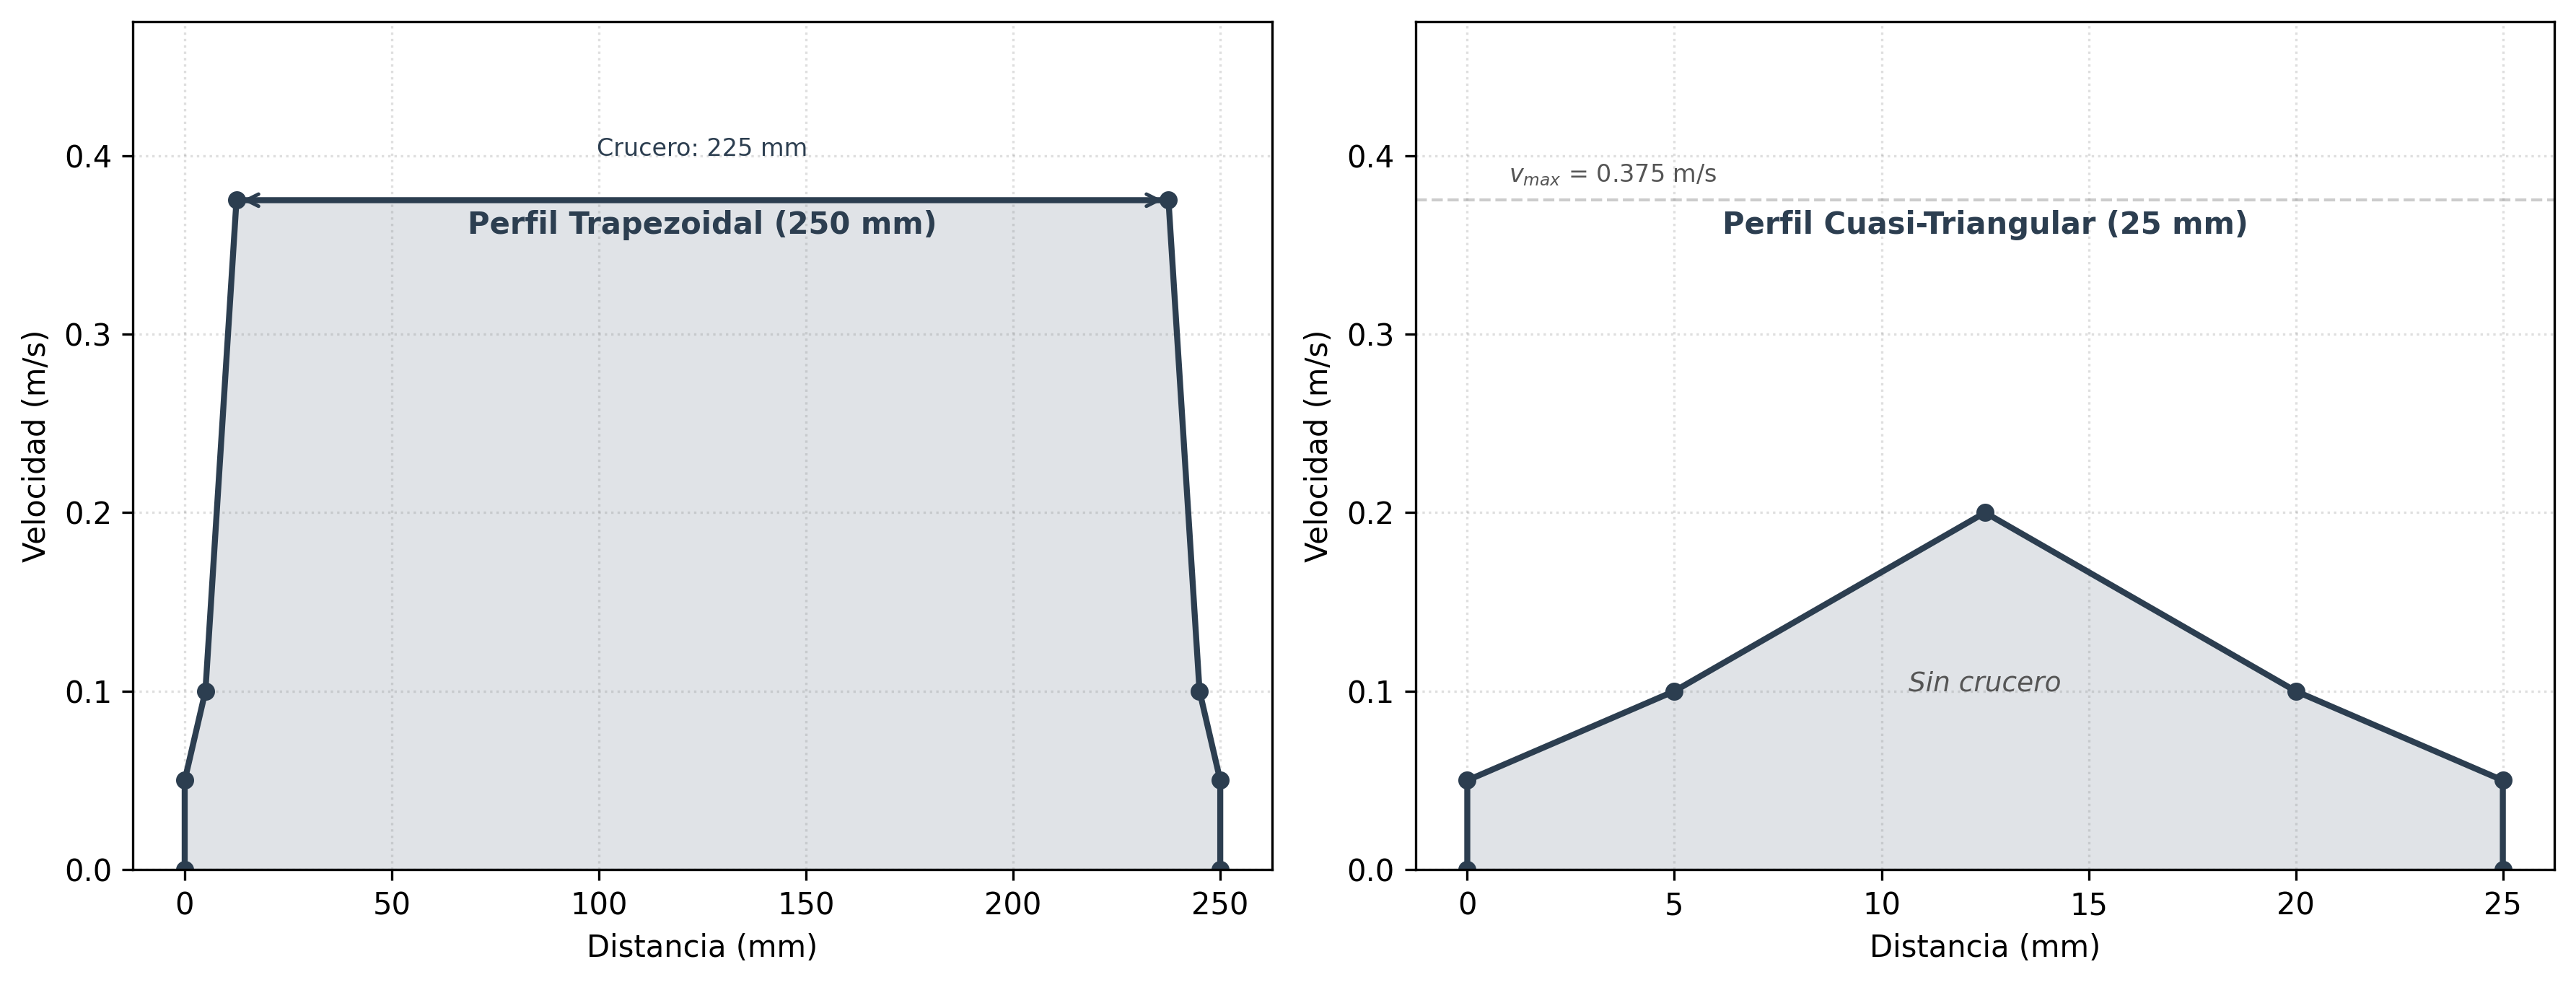
\includegraphics[width=0.7\textwidth]{imagenes/perfil_trapezoidal_triangular.png}
    \caption{Comparación entre perfil trapezoidal (movimientos largos) y triangular (movimientos cortos). Ambos utilizan las mismas aceleraciones, pero el perfil triangular invierte la aceleración en el punto medio}
    \label{fig:perfil_comparacion}
\end{figure}

La velocidad instantánea en cada paso se calcula mediante interpolación lineal dentro de cada zona. El firmware ejecuta este cálculo continuamente en el loop principal a frecuencia superior a 10kHz, actualizando el registro OCR1A del Timer1 que controla la frecuencia de generación de pulsos STEP. La conversión entre velocidad deseada $v$ (en pasos/s) y el valor del registro es:

\begin{equation}
OCR1A = \frac{f_{CPU}}{2 \cdot prescaler \cdot v} - 1 = \frac{1,000,000}{v} - 1
\end{equation}

donde $f_{CPU} = 16$ MHz y prescaler = 8. Por ejemplo, para $v = 5,000$ pasos/s (0.125 m/s), $OCR1A = 199$. El sistema soporta velocidades entre 500 pasos/s (inicio/fin de movimientos) y 15,000 pasos/s (crucero máximo). Velocidades superiores causan jitter excesivo y riesgo de pérdida de pasos.

Para movimientos diagonales que involucran ambos ejes simultáneamente, el firmware sincroniza los perfiles mediante escalamiento proporcional de velocidades. El eje con mayor distancia a recorrer (eje dominante) utiliza su velocidad de crucero nominal, mientras que el eje subordinado escala su velocidad proporcionalmente: $v_{sub} = v_{dom} \times (d_{sub}/d_{dom})$. Este escalamiento se aplica a todas las fases del perfil, garantizando que ambos ejes completen el movimiento en el mismo tiempo y generando trayectorias rectilíneas en el plano XY (Figura \ref{fig:sincronizacion_multieje}). Por ejemplo, para un movimiento de 100mm horizontal y 50mm vertical, el eje horizontal mantiene 0.375 m/s de crucero mientras que el vertical se reduce a 0.1875 m/s, completando ambos en 0.35s.

\begin{figure}[H]
    \centering
    % TODO: Insertar diagrama de sincronización multi-eje
    % Mostrar: dos ejes con diferentes distancias, perfiles escalados, trayectoria rectilínea resultante
    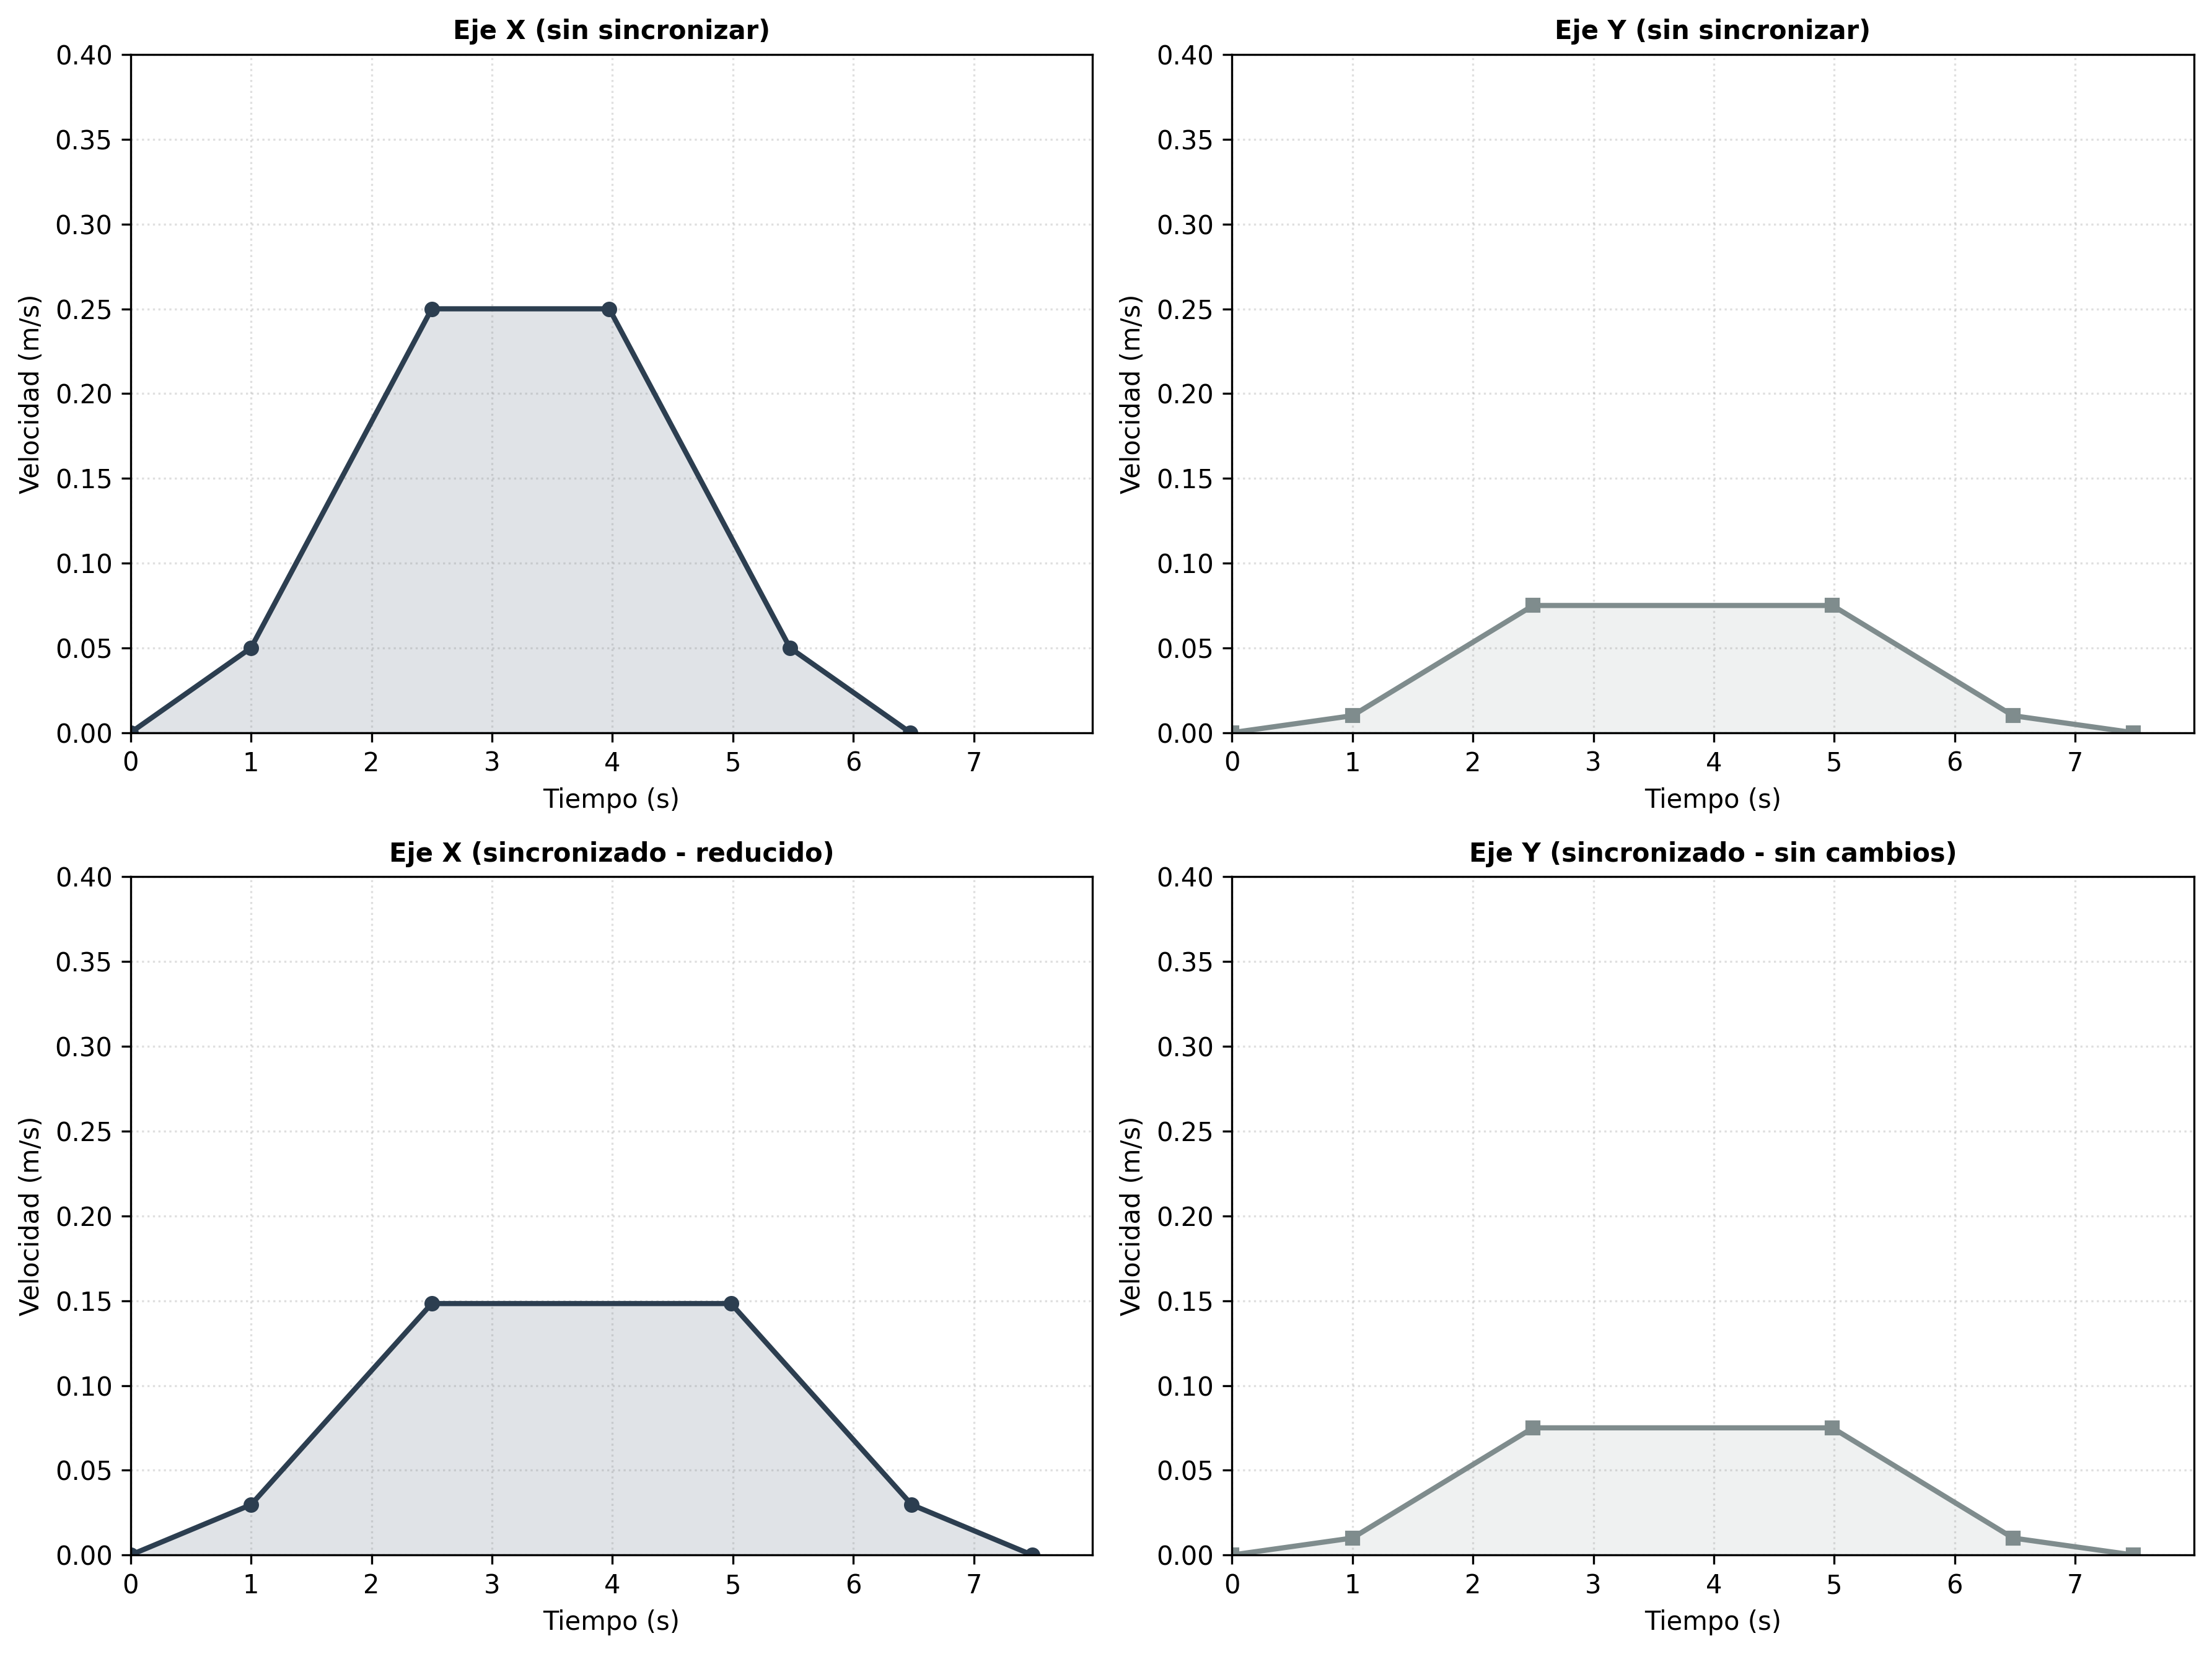
\includegraphics[width=0.7\textwidth]{imagenes/sincronizacion_multieje.png}
    \caption{Sincronización de perfiles de velocidad para movimientos diagonales mediante escalamiento proporcional}
    \label{fig:sincronizacion_multieje}
\end{figure}

El Timer1 genera interrupciones a frecuencia configurable que alternan el estado del pin STEP entre alto y bajo, creando los pulsos necesarios para el driver TB6600. Cada transición alto-bajo constituye un paso del motor. El sistema cuenta los pasos ejecutados y controla la frecuencia de interrupción mediante el registro de comparación OCR1A del timer:

\begin{equation}
f_{step} = \frac{f_{CPU}}{2 \cdot prescaler \cdot (OCR1A + 1)}
\end{equation}

donde $f_{CPU} = 16$ MHz, prescaler = 8, y OCR1A se calcula dinámicamente.

Para una velocidad deseada $v$ en pasos/s, el valor de OCR1A es:

\begin{equation}
OCR1A = \frac{f_{CPU}}{2 \cdot prescaler \cdot v} - 1 = \frac{16000000}{2 \cdot 8 \cdot v} - 1 = \frac{1000000}{v} - 1
\end{equation}

El firmware precalcula y limita OCR1A para evitar overflow y garantizar estabilidad.
La conversión entre pasos de motor y desplazamiento lineal depende de las características mecánicas de cada eje. Los motores NEMA 17 utilizados tienen 200 pasos por revolución, configurados con microstepping 1/8 en los drivers TB6600, resultando en 1600 pasos por revolución efectiva.

\textbf{Eje Horizontal:} Utiliza transmisión por correa dentada GT2 con polea de 20 dientes y paso de 2mm, generando 40mm de avance lineal por revolución del motor. La conversión resulta:
\begin{equation}
\text{Pasos/mm}_H = \frac{1600 \text{ pasos/rev}}{40 \text{ mm/rev}} = 40 \text{ pasos/mm}
\end{equation}

\textbf{Eje Vertical:} Utiliza transmisión por varilla roscada M8 con paso de rosca de 1.25mm, generando 8mm de avance lineal por revolución del motor (rosca de 4 entradas). La conversión resulta:
\begin{equation}
\text{Pasos/mm}_V = \frac{1600 \text{ pasos/rev}}{8 \text{ mm/rev}} = 200 \text{ pasos/mm}
\end{equation}

Estos valores se definen como constantes en el archivo de configuración (system\_config.h) mediante las macros STEPS\_PER\_MM\_H y STEPS\_PER\_MM\_V. El firmware utiliza estas conversiones para traducir comandos en milímetros a cantidad de pasos que debe ejecutar cada motor.

\begin{table}[H]
\centering
\begin{tabular}{|l|c|c|c|c|}
\hline
\textbf{Eje} & \textbf{Transmisión} & \textbf{mm/rev} & \textbf{Pasos/rev} & \textbf{Pasos/mm} \\
\hline
Horizontal & Correa GT2 & 40 & 1600 & 40 \\
\hline
Vertical & Varilla M8 & 8 & 1600 & 200 \\
\hline
\end{tabular}
\caption{Conversiones mecánicas de los ejes de movimiento}
\label{tab:conversiones_mecanicas}
\end{table}


\subsection{Protocolo de Comunicación UART}
% Estructura Comandos


\subsubsection{Manejo de errores y protecciones}

El firmware implementa mecanismos robustos de detección y manejo de errores para garantizar operación segura del sistema mecánico.

Antes de ejecutar cualquier comando, el analizador sintáctico valida sintaxis y rangos. Comandos inválidos retornan código de error inmediatamente sin ejecutar acción, previniendo movimientos peligrosos (Tabla \ref{tab:validacion_comandos}).

\begin{table}[H]
\centering
\small
\begin{tabular}{|l|l|l|}
\hline
Parámetro & Rango válido & Error \\
\hline
Delimitadores & \texttt{<} y \texttt{>} presentes & INVALID\_CMD \\
\hline
Velocidad H & 500 - 15,000 pasos/s & INVALID\_PARAM \\
\hline
Velocidad V & 500 - 12,000 pasos/s & INVALID\_PARAM \\
\hline
Ángulo servo & 10° - 160° & INVALID\_PARAM \\
\hline
Tiempo trayectoria & 0 - 10,000 ms & INVALID\_PARAM \\
\hline
\end{tabular}
\caption{\textit{Validaciones de comandos y rangos permitidos}}
\label{tab:validacion_comandos}
\end{table}

El firmware implementa supervisor de comunicación: si no recibe señal de sincronización (\texttt{HB:1}) del nivel superior durante un período prolongado, asume pérdida de comunicación y ejecuta detención de emergencia automática, deshabilitando todos los motores y entrando en modo seguro hasta recibir comando de reset.

El buffer UART circular (256 bytes) implementa protección contra overflow verificando espacio disponible antes de cada escritura. Si el buffer está lleno, el byte se descarta y se envía error de overflow. La Tabla \ref{tab:codigos_error} lista los códigos de error definidos.

\begin{table}[H]
\centering
\begin{tabular}{|l|p{9cm}|}
\hline
Código & Descripción y causa \\
\hline
INVALID\_CMD & Comando no reconocido o sintaxis incorrecta. \\
\hline
INVALID\_PARAM & Parámetros fuera de rango válido. \\
\hline
LIMIT\_HIT & Movimiento bloqueado por activación de final de carrera. \\
\hline
BUFFER\_OVERFLOW & Buffer UART saturado. \\
\hline
TIMEOUT & Operación excedió tiempo límite configurado. \\
\hline
SYSTEM\_ERROR & Error interno del firmware. \\
\hline
\end{tabular}
\caption{\textit{Códigos de error del firmware}}
\label{tab:codigos_error}
\end{table}

Los finales de carrera se monitorean continuamente. El sistema detecta la activación de cualquier límite y ejecuta inmediatamente la detención de emergencia: deshabilita los drivers (ENABLE = HIGH), detiene la generación de pulsos, envía notificación asíncrona al supervisor indicando el límite activado, y bloquea nuevos comandos de movimiento hacia el lado en el que se encuentra el fin de carrera. Esto previene daños mecánicos por intentos de movimiento en dirección bloqueada.


\section{Sistema de Supervisión y Alta Gestión (Nivel Supervisor)}

\subsection{Arquitectura del Nivel Supervisor}
El software del nivel supervisor se implementa en Python 3 siguiendo una arquitectura modular que separa responsabilidades en capas funcionales específicas. La Figura \ref{fig:arquitectura_modulos_supervisor} muestra la organización de módulos y sus dependencias.

\textbf{Capa de Hardware}: Gestiona la comunicación con el nivel regulatorio y la adquisición de imágenes. El módulo UARTManager implementa comunicación serial mediante puerto USB a 115200 baudios, utilizando callbacks para procesamiento asíncrono de mensajes recibidos del firmware. El módulo CommandManager proporciona métodos de alto nivel para enviar comandos estructurados al nivel regulatorio.

\textbf{Capa de Control}: Coordina el estado global del robot. El módulo RobotController mantiene el seguimiento de posición global mediante acumulación de desplazamientos reportados por el firmware, detecta y maneja eventos mediante callbacks, y gestiona la persistencia de estado en archivos JSON. El módulo CameraManager centraliza el acceso a la cámara USB evitando conflictos de acceso concurrente.

\textbf{Capa de Robot}: Implementa el control del brazo robótico. El módulo ArmController define cuatro posiciones operacionales discretas con ángulos específicos de servomotores y genera trayectorias mediante interpolación lineal.

\textbf{Capa de Procesos}: Define las secuencias de alto nivel del robot. El módulo workflow\_orchestrator implementa los cuatro procesos principales del sistema: homing, calibración del workspace, mapeo del entorno, y cosecha interactiva.

\begin{figure}[H]
    \centering
    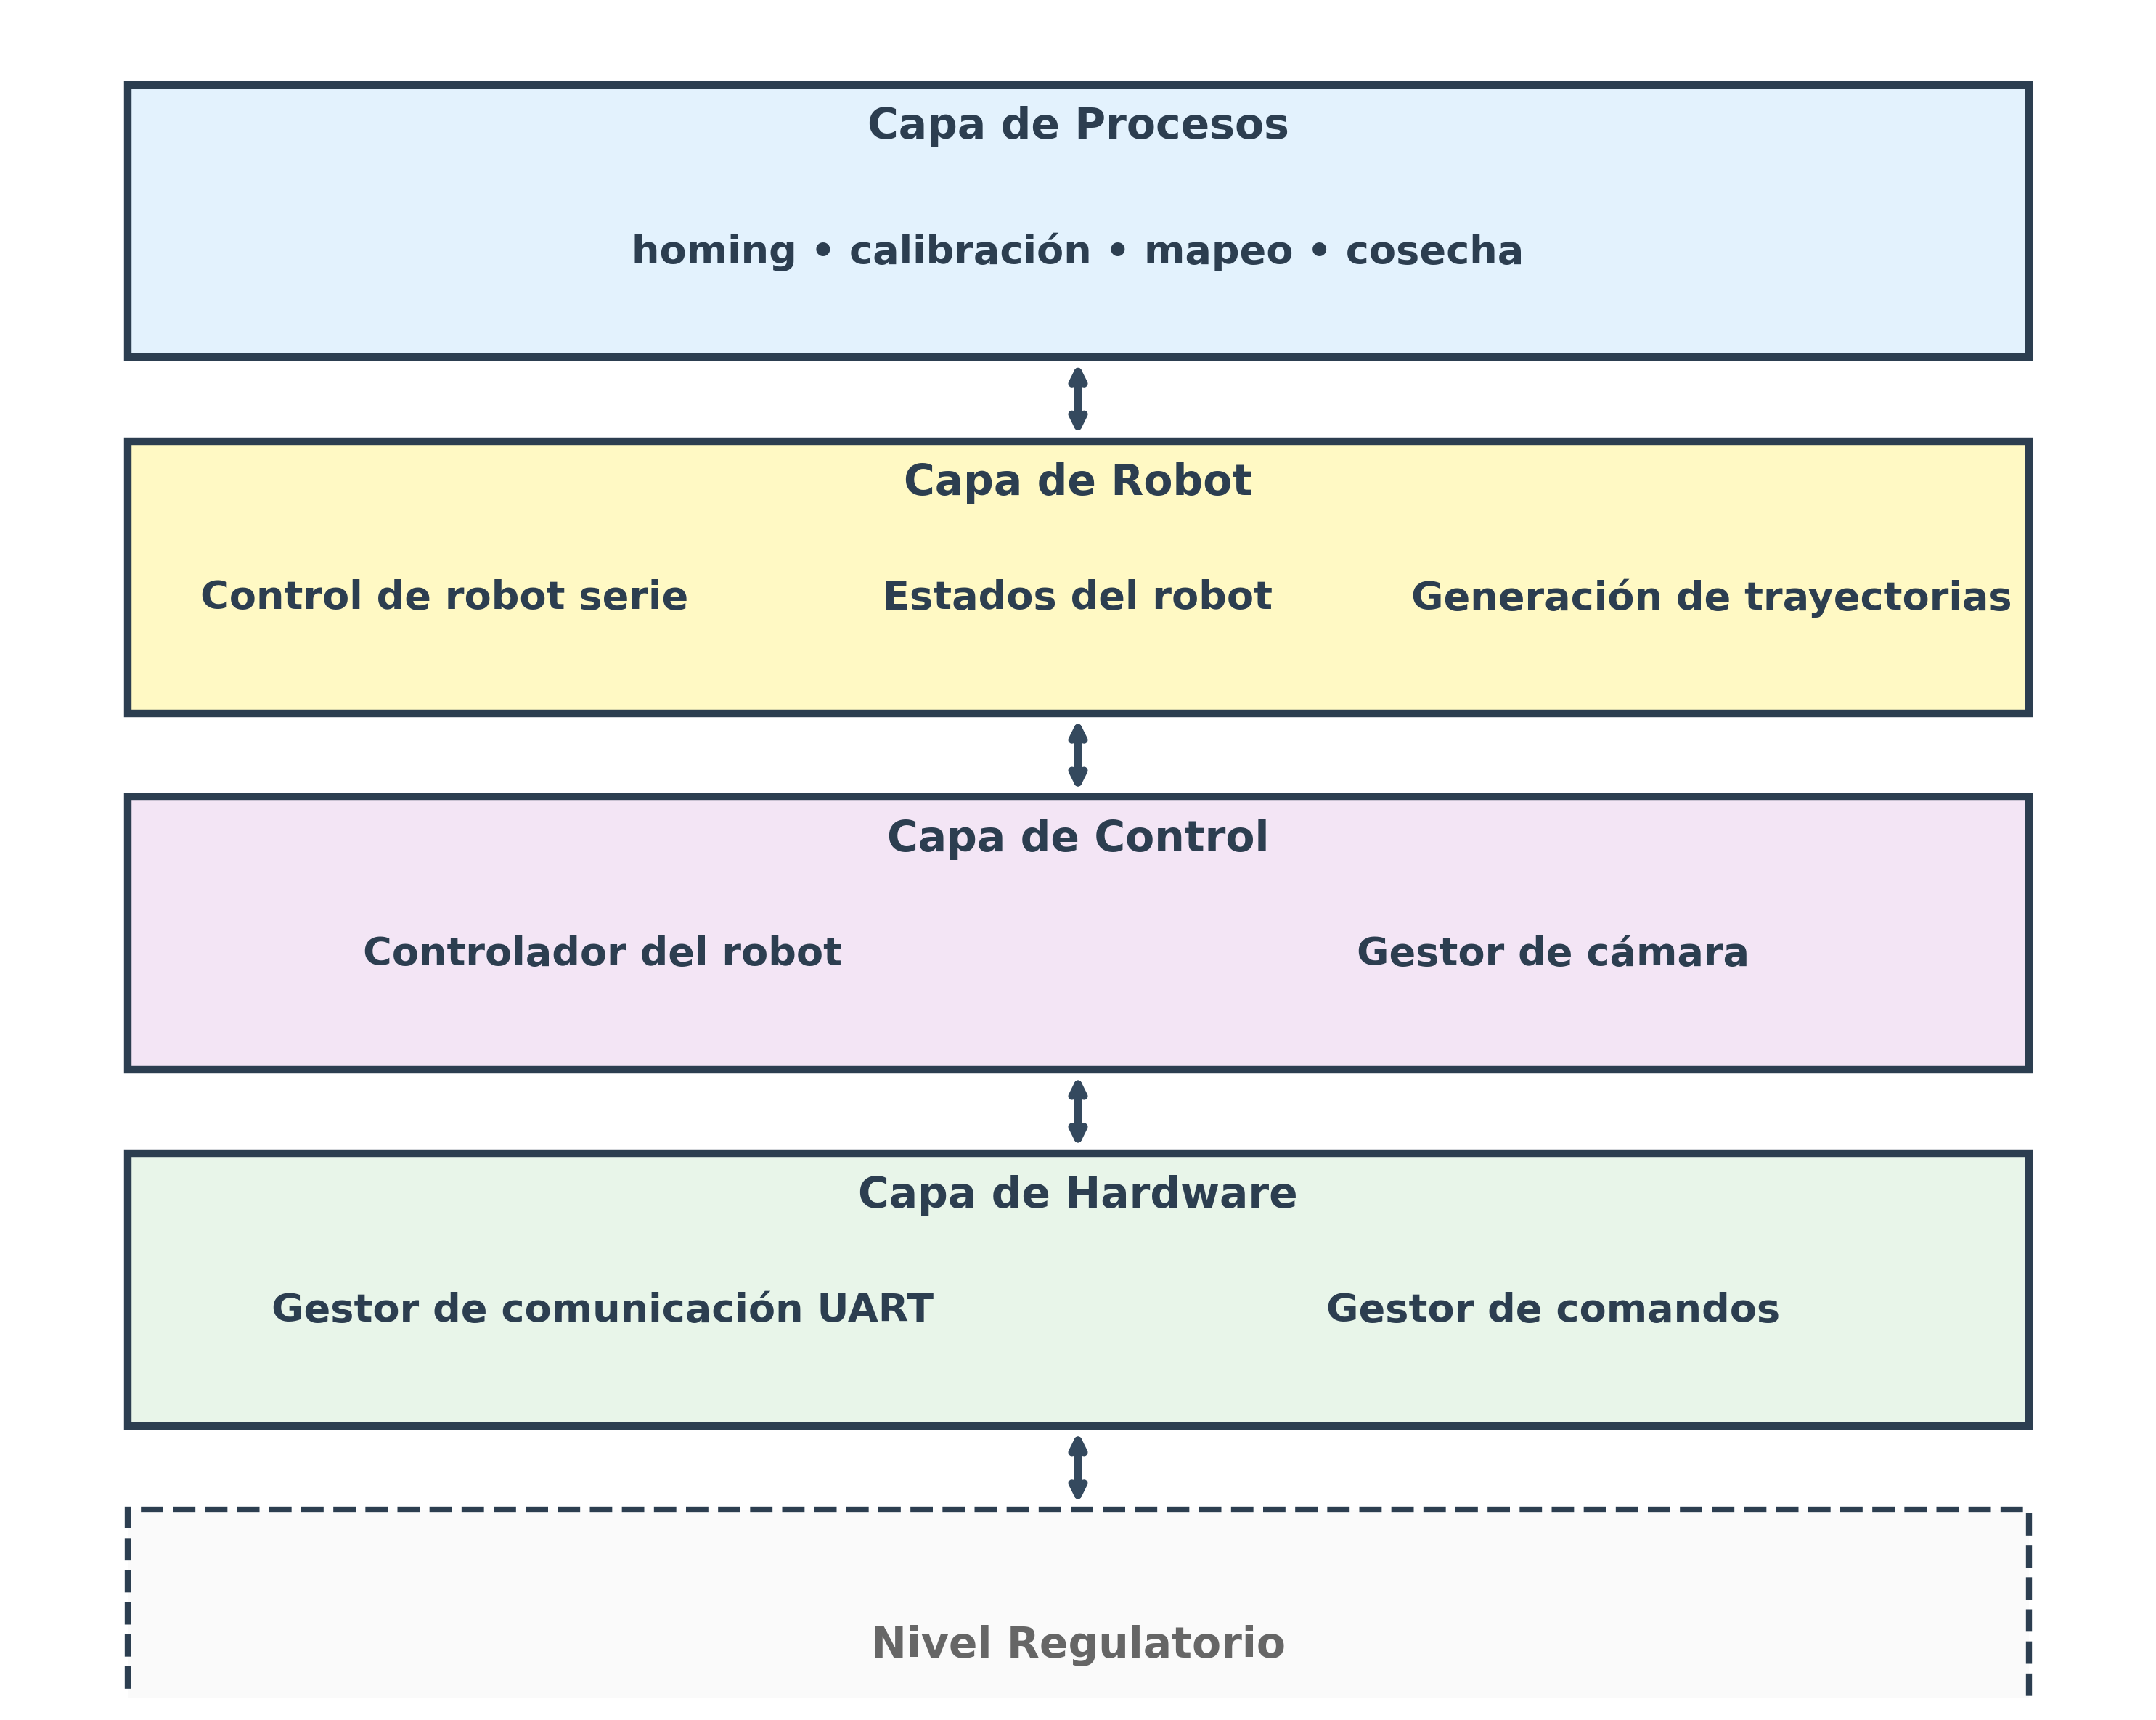
\includegraphics[width=0.8\textwidth]{imagenes/arquitectura_modulos_supervisor.png}
    \caption{\textit{Arquitectura modular del software supervisor mostrando capas y flujo de información}}
    \label{fig:arquitectura_modulos_supervisor}
\end{figure}

\subsection{Hardware Supervisor - Raspberry Pi 4}
\subsubsection{Selección de la Raspberry Pi 5}

El nivel supervisor requiere capacidad de procesamiento simultáneo para inferencia de redes neuronales, gestión de máquina de estados compleja, procesamiento de visión por computadora y comunicación con múltiples subsistemas. Los requerimientos principales incluyen: ejecución de modelos de clasificación de plantas sobre imágenes de 1920x1080 píxeles con latencia inferior a 200ms, procesamiento multi-hilo para gestión concurrente de comunicación UART, captura de cámara e inferencia de IA sin bloqueos, y algoritmos de visión por computadora (detección de marcadores ArUco, segmentación por color, análisis morfológico) sobre imágenes de alta resolución.

La Raspberry Pi 5 con 8GB de RAM fue seleccionada por satisfacer estos requerimientos. El procesador ARM Cortex-A76 quad-core a 2.4GHz (60\% más rápido que RPi 4) ejecuta inferencias de redes neuronales compactas (MobileNet, EfficientNet-Lite) a 5-8 fps. Los 8GB de memoria LPDDR4X-4267 permiten cargar simultáneamente modelos de IA, buffers de imágenes y estructuras de datos sin swapping. La GPU VideoCore VII provee aceleración para operaciones de visión. La conectividad incluye USB 3.0 para cámara (hasta 200 MB/s) y UART hardware para comunicación con el nivel regulatorio. El consumo es de 8-10W típico bajo carga, permitiendo operación continua con disipación pasiva.

La RPi 5 representa el balance óptimo entre capacidad computacional, flexibilidad de desarrollo y costo (\$80 USD). Alternativas como microcontroladores carecen de capacidad para procesamiento de IA, mientras que plataformas más potentes (Jetson Nano, Intel NUC) resultan sobredimensionadas y costosas. El soporte nativo de Linux con Python 3.x y bibliotecas optimizadas (OpenCV-ARM, TensorFlow Lite) facilita el desarrollo e integración del sistema.

% Capacidades Limitaciones



\subsection{Máquina de Estados Supervisora}
El control del brazo robótico se implementa mediante una máquina de estados finitos (FSM) que encapsula la complejidad de las secuencias de movimiento en estados discretos de alto nivel. Esta abstracción permite que los workflows invoquen funcionalidades complejas mediante transiciones simples entre estados.

\subsubsection{Estados Definidos}

El sistema define cuatro estados principales para el brazo, cada uno con configuraciones específicas de servomotores y gripper:

\begin{table}[H]
\centering
\caption{Estados del brazo robótico y sus configuraciones}
\label{tab:estados_brazo}
\begin{tabular}{|l|c|c|c|p{5cm}|}
\hline
\textbf{Estado} & \textbf{Servo 1} & \textbf{Servo 2} & \textbf{Gripper} & \textbf{Propósito} \\
\hline
\texttt{movimiento} & 10° & 10° & Cualquiera & Brazo plegado para desplazamientos XY sin colisiones \\
\hline
\texttt{recoger\_lechuga} & 100° & 80° & Abierto & Posición de aproximación para recolección \\
\hline
\texttt{mover\_lechuga} & 50° & 160° & Cerrado & Transporte con lechuga asegurada \\
\hline
\texttt{depositar\_lechuga} & 90° & 20° & Abierto & Posición de liberación sobre zona de depósito \\
\hline
\end{tabular}
\end{table}

Cada estado representa una configuración completa del sistema brazo-gripper optimizada para una tarea específica dentro del workflow de cosecha.

\begin{figure}[H]
    \centering
    % TODO: Insertar diagrama de estados del brazo con transiciones
    % Mostrar: 4 estados, flechas de transición, condiciones de guarda
    \includegraphics[width=0.9\textwidth]{imagenes/diagrama_estados_brazo.png}
    \caption{Máquina de estados del brazo robótico y transiciones permitidas}
    \label{fig:estados_brazo}
\end{figure}

\subsubsection{Trayectorias Interpoladas}

Las transiciones entre estados no son instantáneas sino que se implementan mediante trayectorias interpoladas linealmente. Para una transición desde un estado A $(s1_A, s2_A, g_A)$ hacia un estado B $(s1_B, s2_B, g_B)$, el sistema genera una secuencia de $N$ puntos intermedios:

\begin{equation}
\theta_i(t) = \theta_i^A + \frac{t}{T} \cdot (\theta_i^B - \theta_i^A), \quad t \in [0, T], \quad i \in \{1, 2\}
\end{equation}

donde $T$ es la duración total del movimiento (típicamente 3-5 segundos) y los puntos se muestrean a 50ms de intervalo. Esta interpolación garantiza movimientos suaves que minimizan vibraciones y cargas mecánicas sobre los servos.

\subsubsection{Gestión del Gripper}

El gripper opera con dos comandos discretos (\texttt{GRIPPER\_OPEN}, \texttt{GRIPPER\_CLOSE}) y timing predefinido:

\begin{itemize}[label=$\bullet$]
    \item \textbf{Apertura}: 2.0 segundos de actuación seguidos de delay de seguridad de 0.3s
    \item \textbf{Cierre}: 2.0 segundos de actuación, verificación de flag de lechuga presente
\end{itemize}

El controlador mantiene un flag interno (\texttt{lettuce\_present}) que indica si el gripper contiene una lechuga, permitiendo validaciones de consistencia en el workflow (ej: no permitir depositar si el flag es \texttt{False}).

\subsubsection{Sincronización con Movimientos XY}

La FSM del brazo está diseñada para coordinarse con el sistema de movimiento XY del nivel regulatorio:

\textbf{Restricción de movimiento seguro:} Los comandos de movimiento XY solo se permiten cuando el brazo está en estado \texttt{movimiento} o \texttt{mover\_lechuga}. Intentar movimientos en otros estados genera una advertencia y una transición automática al estado seguro.

\textbf{Bloqueo durante transiciones:} Mientras el brazo está ejecutando una trayectoria (flag \texttt{is\_executing\_trajectory} = \texttt{True}), se bloquean tanto comandos de movimiento XY como nuevas transiciones de brazo, previniendo condiciones de carrera.

\textbf{Timeouts de seguridad:} Cada transición tiene un timeout máximo (20 segundos). Si la trayectoria no completa en ese tiempo, se genera una excepción y el sistema intenta retornar al estado \texttt{movimiento}.

Este diseño de FSM simplifica dramáticamente la lógica de los workflows de alto nivel, que pueden invocar cambios de estado sin preocuparse por los detalles de timing, interpolación o sincronización con otros subsistemas.

% Transiciones Condiciones


El sistema supervisor implementa mecanismos robustos de manejo de excepciones para garantizar operación continua ante condiciones inesperadas, minimizando interrupciones del servicio.

\subsubsection{Jerarquía de Excepciones}

El sistema define excepciones específicas por tipo de error:

\textbf{Excepciones de comunicación:}
\begin{itemize}[label=$\bullet$]
    \item \texttt{UARTTimeoutException}: Comando enviado sin respuesta en tiempo esperado (>5s)
    \item \texttt{InvalidResponseException}: Respuesta malformada o inconsistente del firmware
    \item \texttt{SerialConnectionLost}: Pérdida de conexión física con Arduino
\end{itemize}

\textbf{Excepciones de movimiento:}
\begin{itemize}[label=$\bullet$]
    \item \texttt{LimitSwitchTriggered}: Activación inesperada de final de carrera durante movimiento
    \item \texttt{PositionDeviationError}: Desviación superior a 5mm entre posición esperada y real
    \item \texttt{HomingFailedException}: Fallo en secuencia de homing (no alcanza límites)
\end{itemize}

\textbf{Excepciones de brazo:}
\begin{itemize}[label=$\bullet$]
    \item \texttt{ArmTransitionTimeout}: Transición de estado no completa en timeout (>20s)
    \item \texttt{InvalidStateTransition}: Intento de transición no permitida por matriz
    \item \texttt{ServoPositionError}: Servo no alcanza posición objetivo (desviación >5°)
\end{itemize}

\textbf{Excepciones de IA:}
\begin{itemize}[label=$\bullet$]
    \item \texttt{CameraAcquisitionFailed}: No se puede adquirir acceso exclusivo a cámara
    \item \texttt{FrameCaptureTimeout}: Captura de imagen excede timeout (>2s)
    \item \texttt{DetectionFailure}: Algoritmo de detección no encuentra features esperados
\end{itemize}

\subsubsection{Estrategias de Recuperación}

Cada tipo de excepción tiene una estrategia de recuperación específica:

\textbf{Recuperación automática (nivel 1):} Para errores transitorios, el sistema intenta recuperación sin intervención:

\begin{enumerate}
    \item \textbf{Timeout UART}: Reenvío del comando hasta 3 veces con backoff exponencial (1s, 2s, 4s)
    \item \textbf{Frame capture timeout}: Reinicio del stream de cámara y reintento de captura
    \item \textbf{Servo position error}: Reenvío de comando de posición con tiempo extendido
\end{enumerate}

\textbf{Recuperación con degradación (nivel 2):} Cuando la recuperación automática falla, el sistema intenta operación degradada:

\begin{enumerate}
    \item \textbf{Detection failure}: Si detector de cintas falla, usa posiciones hardcoded de configuración previa
    \item \textbf{Position deviation}: Ejecuta resincronización forzada desde firmware
    \item \textbf{Arm transition timeout}: Cancela transición, retorna a estado \texttt{movimiento}
\end{enumerate}

\textbf{Parada segura (nivel 3):} Para errores críticos irrecuperables:

\begin{enumerate}
    \item Detiene todos los movimientos en curso (\texttt{EMERGENCY\_STOP})
    \item Intenta mover brazo a posición segura (\texttt{movimiento})
    \item Libera recursos (cámara, conexión serial)
    \item Registra estado completo del sistema en log
    \item Notifica al usuario y espera intervención manual
\end{enumerate}

\subsubsection{Logging Estructurado}

Todas las excepciones se registran con estructura consistente que incluye timestamp preciso, nivel de severidad, módulo origen, tipo de excepción, mensaje descriptivo, contexto completo del sistema (estado actual, comando en curso, variables relevantes), stack trace completo para debugging, y acción de recuperación ejecutada.

Los niveles de logging son:
\begin{itemize}[label=$\bullet$]
    \item \texttt{WARNING}: Excepciones recuperadas automáticamente
    \item \texttt{ERROR}: Excepciones que requieren degradación o reintentos
    \item \texttt{CRITICAL}: Excepciones que causan parada del workflow
\end{itemize}

\subsubsection{Mecanismo de Watchdog}

El sistema implementa un watchdog de alto nivel que monitorea:

\textbf{Liveness del supervisor:} Thread secundario verifica cada 5 segundos que el proceso principal responde a pings internos. Si no hay respuesta en 15s, registra estado y reinicia el supervisor.

\textbf{Detección de deadlocks:} Monitorea tiempo de ejecución de operaciones críticas:
\begin{itemize}[label=$\bullet$]
    \item Movimiento XY: timeout 180s (basado en velocidad y distancia máxima)
    \item Captura + procesamiento IA: timeout 30s
    \item Transición de brazo: timeout 20s
\end{itemize}

Si una operación excede su timeout, el watchdog genera una excepción forzada y libera locks.

\textbf{Heartbeat con nivel regulatorio:} Envío periódico de comando \texttt{HB:1} (heartbeat) cada 30s. Si el regulatorio no responde a 3 heartbeats consecutivos, se asume pérdida de comunicación y se ejecuta parada segura.

\subsubsection{Estrategia de Fail-Safe}

En caso de fallo catastrófico del supervisor (crash de Python, kernel panic, pérdida de alimentación), el nivel regulatorio implementa protección independiente:

\begin{itemize}[label=$\bullet$]
    \item Timeout de heartbeat: Si no recibe \texttt{HB:1} en 90s, ejecuta EMERGENCY\_STOP
    \item Finales de carrera: Siempre activos por hardware, independientes del supervisor
    \item Watchdog de firmware: Reinicio del Arduino si loop principal se bloquea >8s
\end{itemize}

Esta arquitectura de capas redundantes garantiza que el sistema físico nunca queda en estado peligroso, incluso ante fallos múltiples del software de supervisión.


\subsection{Coordinación con Nivel Regulatorio}
La coordinación entre el Nivel Supervisor y el Nivel Regulatorio se realiza mediante un protocolo de comandos estructurados transmitidos por UART. El módulo \texttt{CommandManager} encapsula la lógica de formateado, envío y validación de respuestas.

\subsubsection{Protocolo de Comandos}

Los comandos siguen un formato consistente basado en caracteres ASCII delimitados. Los delimitadores enmarcan cada comando, el separador de dos puntos divide el identificador de los parámetros, y los parámetros múltiples se separan con comas. Este formato mantiene compatibilidad directa con el protocolo implementado en el nivel regulatorio.

\textbf{Comandos de movimiento:}
\begin{itemize}
    \item \texttt{M:x,y} - Movimiento relativo en mm (ej: \texttt{M:50.5,-20.3})
    \item \texttt{V:h\_speed,v\_speed} - Configuración de velocidades en pasos/s
    \item \texttt{XY?} - Consulta de posición actual en mm
    \item \texttt{RP} - Solicitud de progreso de movimiento actual
\end{itemize}

\textbf{Comandos de brazo y gripper:}
\begin{itemize}
    \item \texttt{A:s1,s2,t} - Movimiento de ambos servos a ángulos (s1, s2) en tiempo t (ms)
    \item \texttt{P:num,angle} - Movimiento de servo individual (num=1 o 2)
    \item \texttt{G:O} / \texttt{G:C} - Apertura/cierre de gripper con confirmación
    \item \texttt{GT} - Toggle de gripper (cambio de estado)
    \item \texttt{Q} - Consulta de posiciones actuales de servos
\end{itemize}

\textbf{Comandos de sistema:}
\begin{itemize}
    \item \texttt{S?} - Consulta de estado completo del sistema
    \item \texttt{L?} - Consulta de estado de finales de carrera
    \item \texttt{S} - Emergency stop (detención inmediata de todos los motores)
    \item \texttt{HB:1} - Heartbeat (keep-alive) del supervisor
\end{itemize}

\subsubsection{Gestión de Respuestas}

El \texttt{UARTManager} implementa un sistema de colas para separar respuestas síncronas de notificaciones asíncronas:

\textbf{Respuestas síncronas:} Cada comando enviado espera una respuesta del firmware con prefijo \texttt{RESPONSE} seguido de los datos solicitados, utilizando el mismo formato delimitado. El timeout por defecto es 5 segundos. Si no hay respuesta, se genera \texttt{UARTTimeoutException} y se reintentan hasta 3 veces con backoff exponencial (1s, 2s, 4s).

\textbf{Eventos asíncronos:} El firmware puede enviar notificaciones no solicitadas en cualquier momento:
\begin{itemize}
    \item \texttt{STEPPER\_MOVE\_COMPLETED:...} - Movimiento XY completado con datos de posición
    \item \texttt{LIMIT\_TRIGGERED:tipo} - Final de carrera activado
    \item \texttt{STEPPER\_EMERGENCY\_STOP:...} - Parada de emergencia ejecutada
    \item \texttt{GRIPPER\_OPENED/CLOSED} - Confirmación de acción de gripper
\end{itemize}

Estos mensajes se encolan en \texttt{message\_queue} y son procesados por callbacks registrados.

\subsubsection{Sistema de Callbacks}

El supervisor registra funciones callback para eventos específicos mediante métodos del gestor UART. Se pueden configurar callbacks para progreso de movimiento, finalización de movimiento y activación de límites. Los callbacks se ejecutan en thread separado del lector UART, permitiendo procesamiento no bloqueante. El \texttt{RobotController} utiliza esta funcionalidad para actualizar la posición global automáticamente al completar cada movimiento, manteniendo sincronizado el estado interno sin polling activo.

\subsubsection{Validación de Comandos}

Antes de enviar un comando al firmware, el \texttt{CommandManager} realiza validaciones:

\textbf{Rangos de parámetros:}
\begin{itemize}
    \item Ángulos de servo: 10° - 160° (clampeo automático)
    \item Velocidades: 100 - 8000 pasos/s
    \item Tiempos de trayectoria: 0 - 10000 ms
\end{itemize}

\textbf{Precondiciones de estado:}
\begin{itemize}
    \item Movimientos XY requieren sistema homed (excepto homing mismo)
    \item Comandos de brazo requieren conexión UART activa
    \item Emergency stop siempre permitido (máxima prioridad)
\end{itemize}

Si una validación falla, el comando se rechaza inmediatamente sin enviar al firmware, retornando un diccionario con estado de falla y descripción del error específico.

\subsubsection{Gestión de Concurrencia}

Aunque Python tiene GIL (Global Interpreter Lock), el sistema maneja múltiples threads: el principal ejecuta workflows y lógica de negocio, uno dedicado lee continuamente del puerto serial parseando mensajes y disparando callbacks, y un watchdog monitorea timeouts y liveness del sistema.

Para prevenir race conditions, el acceso a la cola de mensajes está protegido con lock implícito, las escrituras al puerto serial se serializan mediante lock explícito, y la actualización de posición global es atómica (asignación de diccionarios es atómica en CPython).

\subsubsection{Optimización de Latencia}

El sistema minimiza latencia end-to-end mediante buffering asíncrono (buffer de 4096 bytes, suficiente para ~50 mensajes evitando pérdidas durante ráfagas), comandos no bloqueantes (retornan inmediatamente tras validar que el firmware inició la acción, con notificación de completado vía callback asíncrono), y pipelining selectivo (para secuencias predecibles como configurar velocidad + iniciar movimiento, se envían comandos en rápida sucesión sin esperar respuesta individual, reduciendo latencia total de 100ms a ~20ms).

Mediciones muestran latencia típica de 15-30ms desde envío de comando hasta recepción de respuesta, dominada por tiempo de transmisión serial a 115200 baudios más procesamiento en Arduino (<1ms).

La coordinación de movimientos entre el sistema XY del nivel regulatorio y el brazo robótico del supervisor requiere mecanismos sofisticados de sincronización para garantizar operación segura y eficiente.

\subsubsection{Modelo de Coordinación}

El sistema implementa un modelo de coordinación jerárquico:

\textbf{Nivel 1 - Exclusión mutua física:} El brazo solo puede moverse cuando está en configuración segura (\texttt{movimiento} o \texttt{mover\_lechuga}), donde su extensión no interfiere con el workspace XY. Intentar movimiento XY con brazo extendido genera bloqueo preventivo.

\textbf{Nivel 2 - Sincronización de comandos:} Cada subsistema (XY, brazo) ejecuta un solo comando a la vez. Un comando nuevo se encola hasta que el anterior complete, implementando serialización automática.

\textbf{Nivel 3 - Orquestación de workflows:} Los workflows de alto nivel coordinan secuencias complejas mediante wait points explícitos, garantizando completado de acciones previas antes de iniciar las siguientes.

\subsubsection{Mecanismo de Wait Points}

Los workflows utilizan el método \texttt{wait\_for\_action\_completion} para sincronizar operaciones. Este método bloquea la ejecución hasta recibir la notificación correspondiente del firmware o hasta que se cumpla el timeout especificado. Por ejemplo, tras enviar un comando de movimiento XY, el sistema espera la confirmación de completado con un timeout de 180 segundos antes de continuar con la siguiente acción. Internamente:

\begin{enumerate}
    \item Registra el tipo de acción esperada en queue de espera
    \item Thread de lectura UART monitorea mensajes entrantes
    \item Al detectar mensaje de completado, desbloquea el wait point
    \item Retorna True si completó, genera excepción si timeout
\end{enumerate}

\subsubsection{Coordinación Brazo-XY en Workflows}

El workflow de cosecha implementa una secuencia de coordinación en cuatro etapas: primero mueve el sistema XY a la posición de la lechuga detectada y espera confirmación con timeout de 180 segundos; segundo, cambia el brazo a posición de recolección extendida y espera su confirmación con timeout de 20 segundos; tercero, activa el gripper y retrae el brazo a posición de transporte seguro verificando el cambio de estado; finalmente, mueve el sistema XY a la posición de depósito (ahora seguro porque el brazo está retraído) y espera la confirmación del movimiento. Cada transición garantiza que el estado anterior está consolidado antes de proceder.

\subsubsection{Gestión de Timeouts Adaptativos}

Los timeouts se calculan dinámicamente basados en la operación:

\textbf{Movimientos XY:} Timeout = $\frac{d_{euclidiana}}{v_{min}} \times 1.5 + 10s$, donde $d_{euclidiana}$ es la distancia a recorrer y $v_{min}$ la velocidad mínima configurada. El factor 1.5 provee margen para aceleraciones/deceleraciones.

\textbf{Transiciones de brazo:} Timeout fijo de 20s (trayectoria más larga: \texttt{movimiento} $\rightarrow$ \texttt{recoger\_lechuga}: 3-5s nominales).

\textbf{Operaciones de IA:} Timeout variable según módulo:
\begin{itemize}
    \item Detección ArUco: 5s (procesamiento simple)
    \item Clasificación de planta: 15s (inferencia de red neuronal)
    \item Escaneo completo de tubo: 60s (múltiples capturas + procesamiento)
\end{itemize}

\subsubsection{Sincronización con Módulos de IA}

Los módulos de visión requieren coordinación especial:

\textbf{Adquisición de cámara:} Implementa patrón acquire/release con lock mediante el gestor de cámara. El sistema bloquea el acceso hasta que la cámara esté disponible, captura el frame requerido dentro de un bloque protegido, y siempre libera el recurso al finalizar (incluso si hay excepciones), garantizando que otros módulos puedan acceder posteriormente.

\textbf{Estabilización post-movimiento:} Tras un movimiento XY, se espera 500ms adicionales antes de capturar imagen para permitir que vibraciones mecánicas se disipen y la imagen sea nítida.

\textbf{Sincronización de iluminación:} Si hay control de iluminación externa (futuro), se sincronizan ciclos de captura con encendido/apagado de LEDs para consistencia.

\subsubsection{Detección y Resolución de Deadlocks}

El sistema implementa detección proactiva de deadlocks potenciales:

\textbf{Timeout watchdog:} Thread independiente monitorea duración de operaciones críticas. Si una operación excede 3x su timeout nominal, se asume deadlock y se fuerza liberación de recursos.

\textbf{Liveness probes:} El supervisor envía heartbeat (\texttt{HB:1}) cada 30s al regulatorio. Si no recibe ACK en 90s (3 intentos), asume desconexión y ejecuta reset de comunicación.

\textbf{Detección de starvation:} Si un módulo espera acceso a cámara por más de 60s, se registra advertencia y se fuerza liberación del lock actual para prevenir bloqueo permanente.

\subsubsection{Optimización de Latencia Total}

Para minimizar tiempo total de workflows:

\textbf{Pipelining cuando es seguro:} En secuencias donde el siguiente comando es predecible y seguro, se puede iniciar sin esperar completado del anterior. Ejemplo: Configurar velocidad + iniciar movimiento se puede pipeline (la configuración es instantánea).

\textbf{Movimientos simultáneos:} El firmware permite movimiento simultáneo de ejes X e Y (comando \texttt{M:x,y} es atómico). El supervisor aprovecha esto para movimientos diagonales en un solo comando vs dos secuenciales.

\textbf{Transiciones de brazo paralelas a procesamiento IA:} Mientras el brazo ejecuta una trayectoria (3-5s), el supervisor puede iniciar procesamiento de imagen capturada previamente, solapando operaciones para mejor throughput.

Estas optimizaciones reducen el tiempo de cosecha de una planta de ~30s (secuencial puro) a ~15-20s (con solapamiento inteligente), mejorando significativamente la productividad del sistema.

% Recuperacion Fallas



\section{Inteligencia Artificial y Visión por Computadora}

\subsection{Arquitectura General del Sistema de IA}
% Arquitectura Ia


\subsubsection{Algoritmo de detección de cintas}

El algoritmo de detección de cintas de referencia explota el alto contraste entre la cinta negra y el fondo claro mediante procesamiento en el canal de valor (V) del espacio HSV. Esta elección se fundamenta en la invariancia del canal V ante cambios en la tonalidad cromática de la iluminación, propiedad demostrada en el marco teórico (Sección 2.2.1).

\textbf{Etapa 1: Conversión al espacio HSV}

El proceso inicia con la captura de una imagen RGB de la región donde se espera encontrar el marcador. La imagen se transforma al espacio HSV aplicando las ecuaciones de conversión estándar, y se extrae el canal V que representa el brillo de cada píxel.

\textbf{Etapa 2: Umbralización inversa}

Sobre el canal V se aplica umbralización inversa con valor de referencia de 50, operación que asigna valor máximo (blanco) a los píxeles oscuros y valor nulo (negro) a los píxeles claros. Matemáticamente:

\begin{equation}
I_{bin}(x,y) = \begin{cases}
255 & \text{si } I_V(x,y) < 50 \\
0 & \text{si } I_V(x,y) \geq 50
\end{cases}
\end{equation}

El valor de umbral 50 se determinó experimentalmente mediante análisis del imágenes representativas, identificando el punto que maximiza la separación entre la distribución de intensidades de las cintas negras y la distribución de intensidades del fondo blanco.

\textbf{Etapa 3: Detección de contornos}

Sobre la imagen binaria resultante se ejecuta el algoritmo de detección de contornos de Suzuki-Abe, obteniendo las fronteras de todas las regiones oscuras detectadas. Los contornos se filtran aplicando un criterio de área mínima de 500 píxeles, eliminando elementos espurios correspondientes a ruido o pequeñas sombras. Este umbral se estableció considerando que una cinta de 18 milímetros de ancho a 200 milímetros de distancia subtiende aproximadamente 120 píxeles de ancho en la imagen, resultando en áreas típicas superiores a 3000 píxeles para segmentos de cinta de longitud razonable.

\subsubsection{Evaluación de calidad del contorno}

Los contornos que superan el filtrado de área se someten a evaluación de calidad para discriminar entre cintas de referencia genuinas y otros elementos oscuros presentes en la escena (como plantas o vasos). La evaluación se basa en el análisis de la región basal del contorno, definida como el 10 por ciento inferior de su rectángulo delimitador.

Para cada contorno candidato se calcula su rectángulo delimitador $(x, y, w, h)$, donde $(x,y)$ representa la esquina inferior izquierda, $w$ el ancho y $h$ la altura. La región basal se define entonces como:

\begin{equation}
R_{base} = \{(x',y') : x \leq x' < x+w, \, y+0.9h \leq y' < y+h\}
\end{equation}

Se calcula la fracción de píxeles blancos en esta región respecto al total de píxeles de la región:

\begin{equation}
Q_{base} = \frac{1}{|R_{base}|} \sum_{(x,y) \in R_{base}} \frac{I_{bin}(x,y)}{255}
\end{equation}

donde $|R_{base}|$ denota el número de píxeles en la región. Un valor $Q_{base}$ cercano a 1 indica que la región basal del contorno es consistentemente oscura, característica de las cintas de referencia cuyo borde inferior es nítido y bien definido. Valores inferiores indican contornos de objetos con bases irregulares o discontinuas, como plantas con hojas que no presentan un borde horizontal claro.

Esta métrica resulta efectiva para distinguir cintas de otros elementos oscuros: las cintas genuinas presentan típicamente $Q_{base} > 0.8$, mientras que plantas u otros objetos tienen $Q_{base} < 0.5$. Se establece un umbral de aceptación de 0.7 como compromiso entre sensibilidad y especificidad.

\subsubsection{Sistema de evaluación ponderada}

Cuando múltiples contornos cumplen los criterios de área mínima y calidad basal, se implementa un sistema de evaluación ponderada que considera tres factores para seleccionar el mejor candidato.

El primer factor evalúa el área del contorno normalizada respecto a los límites mínimo y máximo esperados:

\begin{equation}
S_{área} = \frac{A - A_{min}}{A_{max} - A_{min}}
\end{equation}

donde $A$ es el área del contorno, $A_{min} = 500$ píxeles y $A_{max} = 50000$ píxeles. Este factor favorece contornos con áreas intermedias, descartando elementos excesivamente pequeños (ruido) o excesivamente grandes (probablemente no corresponden a una cinta individual).

El segundo factor evalúa la posición del centroide del contorno respecto al centro de la imagen:

\begin{equation}
S_{posición} = 1 - \frac{|c_x - x_{centro}|}{W_{imagen}/2}
\end{equation}

donde $c_x$ es la coordenada horizontal del centroide, $x_{centro}$ es la coordenada horizontal del centro de la imagen, y $W_{imagen}$ es el ancho total de la imagen. Este factor favorece contornos cercanos al centro, bajo la hipótesis de que el sistema de control posiciona aproximadamente el robot frente a la cinta objetivo, resultando en desviaciones pequeñas.

El tercer factor corresponde directamente a la calidad basal $Q_{base}$ calculada previamente, que favorece contornos con bordes inferiores bien definidos.

La puntuación total se calcula como combinación lineal ponderada de estos tres factores:

\begin{equation}
P_{total} = w_1 \cdot S_{área} + w_2 \cdot S_{posición} + w_3 \cdot Q_{base}
\end{equation}

Los pesos se establecieron como $w_1 = 0.3$, $w_2 = 0.4$ y $w_3 = 0.3$, otorgando mayor importancia a la posición dado que las desviaciones típicas son inferiores a 50 milímetros, resultando en centroides próximos al centro de la imagen. El contorno con mayor puntuación total se selecciona como la cinta de referencia.

\begin{figure}[H]
\centering
\begin{subfigure}[b]{0.48\textwidth}
    \centering
    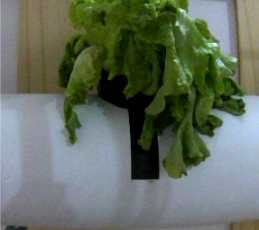
\includegraphics[width=\textwidth]{imagenes/detector_marcadores_1_original.png}
    \caption{Imagen RGB original capturada}
\end{subfigure}
\hfill
\begin{subfigure}[b]{0.48\textwidth}
    \centering
    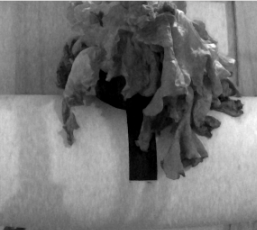
\includegraphics[width=\textwidth]{imagenes/detector_marcadores_2_canal_v.png}
    \caption{Canal V extraído (brillo)}
\end{subfigure}

\vspace{0.3cm}

\begin{subfigure}[b]{0.48\textwidth}
    \centering
    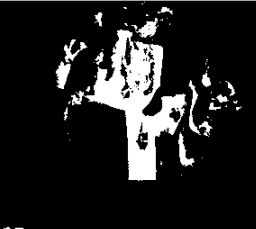
\includegraphics[width=\textwidth]{imagenes/detector_marcadores_3_binario.png}
    \caption{Umbralización binaria inversa (T=50)}
\end{subfigure}
\hfill
\begin{subfigure}[b]{0.48\textwidth}
    \centering
    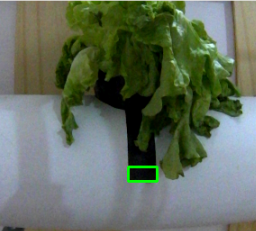
\includegraphics[width=\textwidth]{imagenes/detector_marcadores_4_contornos.png}
    \caption{Contornos detectados con evaluación ponderada}
\end{subfigure}

\caption{\textit{Secuencia de procesamiento del detector de cintas mostrando las transformaciones sucesivas de la imagen}}
\label{fig:proceso_marcadores}
\end{figure}


\subsection{Sistema de Visión Artificial}
% Hardware Camara


% Preprocesamiento


\subsection{Clasificación Basada en Análisis Morfológico}

La clasificación morfológica de objetos utiliza características geométricas y estadísticas extraídas de contornos e imágenes para asignar categorías a elementos detectados. A diferencia de métodos de aprendizaje profundo, este enfoque se fundamenta en reglas explícitas derivadas del conocimiento del dominio y análisis estadístico de datos representativos.

\subsubsection{Fundamentos de Clasificación por Umbrales}

El método más directo de clasificación morfológica establece límites de decisión basados en valores de descriptores geométricos. Para un descriptor $d$ y un conjunto de clases $\mathcal{C} = \{c_1, c_2, ..., c_n\}$, la regla de clasificación se define como:

\begin{equation}
\text{Clase}(x) = c_i \quad \text{si} \quad t_{i-1} < d(x) \leq t_i
\end{equation}

donde $t_0, t_1, ..., t_n$ son umbrales que particionan el espacio de características.

\textbf{Clasificación por Área}

Para objetos que se diferencian principalmente por tamaño, el área en píxeles constituye un descriptor efectivo:

\begin{equation}
\text{Clase}(C) = \begin{cases}
\text{Pequeño} & \text{si } A < t_1 \\
\text{Mediano} & \text{si } t_1 \leq A < t_2 \\
\text{Grande} & \text{si } A \geq t_2
\end{cases}
\end{equation}

La robustez del método depende de la separabilidad entre clases. La distancia entre centroides de clases adyacentes debe ser significativa respecto a la dispersión intra-clase.

\subsubsection{Análisis Estadístico para Determinación de Umbrales}

La selección óptima de umbrales requiere análisis estadístico de una base de datos representativa de cada clase.

\textbf{Parámetros Estadísticos por Clase}

Para cada clase $c_i$, se calculan la media y desviación estándar del descriptor de interés:

\begin{equation}
\mu_i = \frac{1}{N_i}\sum_{j=1}^{N_i} d_j
\end{equation}

\begin{equation}
\sigma_i = \sqrt{\frac{1}{N_i-1}\sum_{j=1}^{N_i}(d_j - \mu_i)^2}
\end{equation}

donde $N_i$ es el número de muestras de la clase $i$, $\mu_i$ es la media y $\sigma_i$ la desviación estándar del descriptor $d$.

\textbf{Determinación de Umbrales mediante Análisis de Distribuciones}

Asumiendo distribuciones normales para cada clase:

\begin{equation}
P(d|c_i) = \frac{1}{\sigma_i\sqrt{2\pi}} \exp\left(-\frac{(d-\mu_i)^2}{2\sigma_i^2}\right)
\end{equation}

Para distribuciones con igual varianza ($\sigma_i = \sigma_{i+1} = \sigma$), el umbral óptimo entre clases consecutivas es:

\begin{equation}
t_i^* = \frac{\mu_i + \mu_{i+1}}{2}
\end{equation}

Este umbral minimiza la probabilidad de error cuando las clases tienen igual probabilidad a priori y varianzas similares.

\subsubsection{Clasificación Multi-Criterio con Ratios de Color}

Cuando un único descriptor geométrico no proporciona separabilidad suficiente, se emplean múltiples características simultáneamente. En el contexto de agricultura de precisión, los ratios de color resultan particularmente efectivos.

\textbf{Espacio de Características de Color}

Dado un contorno, se calculan ratios que cuantifican la proporción de diferentes componentes cromáticos:

\begin{equation}
r_{verde} = \frac{N_{píxeles\_verdes}}{N_{píxeles\_totales}}
\end{equation}

\begin{equation}
r_{negro} = \frac{N_{píxeles\_negros}}{N_{píxeles\_totales}}
\end{equation}

donde $N_{píxeles\_totales} = N_{píxeles\_verdes} + N_{píxeles\_negros} + N_{píxeles\_otros}$.

Cada objeto se representa como un vector en el espacio de características:

\begin{equation}
\mathbf{x} = [r_{verde}, r_{negro}, I_{media}]^T
\end{equation}

donde $I_{media}$ es la intensidad promedio de píxeles internos.

\textbf{Prototipos de Clase}

Para cada clase $c_i$, se define un prototipo mediante las medias de los descriptores:

\begin{equation}
\boldsymbol{\mu}_i = [\mu_{verde,i}, \mu_{negro,i}, \mu_{intensidad,i}]^T
\end{equation}

\textbf{Desviaciones Estándar por Clase}

Las variaciones dentro de cada clase se cuantifican mediante:

\begin{equation}
\boldsymbol{\sigma}_i = [\sigma_{verde,i}, \sigma_{negro,i}, \sigma_{intensidad,i}]^T
\end{equation}

\subsubsection{Distancia Euclidiana Normalizada}

Para clasificar un objeto nuevo, se calcula su distancia a cada prototipo de clase. La normalización por desviación estándar garantiza que descriptores con diferentes rangos contribuyan equitativamente.

\textbf{Distancia Normalizada}

La distancia de un objeto $\mathbf{x}$ al prototipo de la clase $c_i$ se define como:

\begin{equation}
D_i(\mathbf{x}) = \sqrt{\sum_{k=1}^{m} \left(\frac{x_k - \mu_{k,i}}{\sigma_{k,i} + \epsilon}\right)^2}
\end{equation}

donde:
\begin{itemize}
\item $m$ es el número de descriptores (ej. 3 para verde, negro, intensidad)
\item $x_k$ es el valor del descriptor $k$ para el objeto
\item $\mu_{k,i}$ es la media del descriptor $k$ para la clase $i$
\item $\sigma_{k,i}$ es la desviación estándar del descriptor $k$ para la clase $i$
\item $\epsilon$ es un término pequeño (ej. $10^{-6}$) para evitar división por cero
\end{itemize}

\textbf{Regla de Clasificación por Mínima Distancia}

El objeto se asigna a la clase con menor distancia normalizada:

\begin{equation}
\text{Clase}(\mathbf{x}) = \arg\min_{i} D_i(\mathbf{x})
\end{equation}

Este criterio implementa un clasificador de vecino más cercano en el espacio normalizado.

\textbf{Cálculo de Confianza}

La confianza de la clasificación se deriva de las distancias relativas:

\begin{equation}
\text{Confianza} = 1 - \frac{D_{min}}{D_{max} + D_{min}}
\end{equation}

donde $D_{min}$ es la distancia a la clase predicha y $D_{max}$ la distancia a la clase más lejana. Valores cercanos a 1 indican alta confianza; valores cercanos a 0.5 sugieren ambigüedad.

Para mejorar robustez, la confianza se limita:

\begin{equation}
\text{Confianza}_{final} = \max(0.3, \min(1.0, \text{Confianza}))
\end{equation}

garantizando un rango $[0.3, 1.0]$.

\subsubsection{Ejemplo: Clasificación de Cultivos}

Para un sistema de clasificación de tubos de cultivo con tres clases:

\begin{itemize}
\item \textbf{LECHUGAS}: Alto ratio verde ($r_{verde} > 0.40$)
\item \textbf{PLANTINES}: Ratio verde moderado, alto ratio negro
\item \textbf{VASOS} (vacíos): Muy bajo ratio verde, alto ratio negro
\end{itemize}

\textbf{Prototipos Estimados}

A partir de un dataset de entrenamiento:

\begin{equation}
\boldsymbol{\mu}_{LECHUGAS} = [0.65, 0.35, 120]^T, \quad \boldsymbol{\sigma}_{LECHUGAS} = [0.15, 0.15, 30]^T
\end{equation}

\begin{equation}
\boldsymbol{\mu}_{PLANTINES} = [0.45, 0.55, 90]^T, \quad \boldsymbol{\sigma}_{PLANTINES} = [0.15, 0.15, 25]^T
\end{equation}

\begin{equation}
\boldsymbol{\mu}_{VASOS} = [0.05, 0.95, 50]^T, \quad \boldsymbol{\sigma}_{VASOS} = [0.10, 0.10, 20]^T
\end{equation}

\textbf{Clasificación de Muestra}

Dado un objeto con descriptores $\mathbf{x} = [0.60, 0.40, 115]^T$:

\begin{equation}
D_{LECHUGAS} = \sqrt{\left(\frac{0.60-0.65}{0.15}\right)^2 + \left(\frac{0.40-0.35}{0.15}\right)^2 + \left(\frac{115-120}{30}\right)^2} = 0.47
\end{equation}

\begin{equation}
D_{PLANTINES} = \sqrt{\left(\frac{0.60-0.45}{0.15}\right)^2 + \left(\frac{0.40-0.55}{0.15}\right)^2 + \left(\frac{115-90}{25}\right)^2} = 1.52
\end{equation}

\begin{equation}
D_{VASOS} = \sqrt{\left(\frac{0.60-0.05}{0.10}\right)^2 + \left(\frac{0.40-0.95}{0.10}\right)^2 + \left(\frac{115-50}{20}\right)^2} = 8.56
\end{equation}

La clase predicha es LECHUGAS ($D_{min} = 0.47$) con confianza:

\begin{equation}
\text{Confianza} = 1 - \frac{0.47}{8.56 + 0.47} = 0.95
\end{equation}

\subsubsection{Análisis de Separabilidad de Clases}

La efectividad de un conjunto de descriptores para clasificación se cuantifica mediante métricas de separabilidad.

\textbf{Criterio de Fisher}

Mide la razón entre varianza inter-clase e intra-clase para un descriptor $d$:

\begin{equation}
J_F = \frac{(\mu_1 - \mu_2)^2}{\sigma_1^2 + \sigma_2^2}
\end{equation}

Valores altos de $J_F$ indican buena separabilidad. Para múltiples clases:

\begin{equation}
J_F = \frac{\sum_{i=1}^{C} N_i(\mu_i - \mu_{global})^2}{\sum_{i=1}^{C} N_i \sigma_i^2}
\end{equation}

donde $\mu_{global}$ es la media global ponderada.

\textbf{Índice de Solapamiento}

Para distribuciones gaussianas, el solapamiento entre clases $i$ y $j$ se aproxima:

\begin{equation}
\text{Overlap}_{i,j} \approx 2\Phi\left(-\frac{|\mu_i - \mu_j|}{2\sqrt{\sigma_i^2 + \sigma_j^2}}\right)
\end{equation}

donde $\Phi$ es la función de distribución acumulada normal estándar. Valores cercanos a 0 indican separación perfecta; valores cercanos a 1 indican fuerte solapamiento.

\subsubsection{Validación Estadística del Clasificador}

\textbf{Exactitud Estimada}

La exactitud de un clasificador se define como:

\begin{equation}
\text{Exactitud} = \frac{N_{correctas}}{N_{total}}
\end{equation}

donde $N_{correctas}$ es el número de clasificaciones correctas y $N_{total}$ el tamaño del conjunto de prueba.

\textbf{Intervalo de Confianza}

El intervalo de confianza al 95\% para la exactitud es:

\begin{equation}
\text{IC}_{95\%} = \hat{p} \pm 1.96\sqrt{\frac{\hat{p}(1-\hat{p})}{n}}
\end{equation}

donde $\hat{p}$ es la exactitud observada y $n$ el tamaño de la muestra de prueba.

\textbf{Tamaño de Muestra Requerido}

Para estimar la exactitud con error máximo $E$ y nivel de confianza del 95\%:

\begin{equation}
n_{min} = \left(\frac{1.96 \cdot \sqrt{\hat{p}(1-\hat{p})}}{E}\right)^2
\end{equation}

Por ejemplo, para $E = 0.05$ (error de 5\%) y $\hat{p} = 0.9$:

\begin{equation}
n_{min} = \left(\frac{1.96 \cdot \sqrt{0.9 \cdot 0.1}}{0.05}\right)^2 \approx 139
\end{equation}

Se requieren al menos 139 muestras de prueba.

\subsubsection{Robustez y Generalización}

\textbf{Validación Cruzada k-fold}

Para evaluar la generalización del clasificador, se emplea validación cruzada:

\begin{enumerate}
\item Dividir dataset en $k$ particiones de igual tamaño (típicamente $k=5$ o $k=10$)
\item Para $i = 1$ a $k$:
   \begin{itemize}
   \item Usar partición $i$ como conjunto de prueba
   \item Usar restantes $k-1$ particiones para calcular prototipos ($\boldsymbol{\mu}_i$, $\boldsymbol{\sigma}_i$)
   \item Evaluar exactitud en partición $i$
   \end{itemize}
\item Calcular exactitud promedio
\end{enumerate}

La exactitud estimada por validación cruzada es:

\begin{equation}
\text{Exactitud}_{CV} = \frac{1}{k}\sum_{i=1}^{k} \text{Exactitud}_i
\end{equation}

Esta métrica proporciona una estimación más realista del desempeño en datos nuevos que la evaluación en un único conjunto de prueba.

\textbf{Sensibilidad a Variaciones}

La robustez ante ruido se evalúa añadiendo perturbaciones controladas a los descriptores:

\begin{equation}
d_{ruidoso} = d_{verdadero} + \mathcal{N}(0, \sigma_{ruido}^2)
\end{equation}

donde $\mathcal{N}(0, \sigma_{ruido}^2)$ es ruido gaussiano con desviación estándar $\sigma_{ruido}$.

Un clasificador robusto mantiene exactitud alta incluso con $\sigma_{ruido}$ moderado. La degradación de desempeño se cuantifica como:

\begin{equation}
\Delta\text{Exactitud} = \text{Exactitud}_{limpio} - \text{Exactitud}_{ruidoso}
\end{equation}

Degradaciones $\Delta\text{Exactitud} < 0.1$ (10\%) indican robustez aceptable.

\subsubsection{Ventajas y Limitaciones del Enfoque Morfológico}

\textbf{Ventajas:}
\begin{itemize}
\item \textbf{Interpretabilidad}: Reglas de decisión explícitas y comprensibles basadas en características físicas medibles
\item \textbf{Eficiencia computacional}: Cálculos geométricos y estadísticos simples, ejecución en tiempo real en hardware embebido
\item \textbf{Pocos datos requeridos}: Decenas a cientos de muestras por clase, vs. miles requeridos por aprendizaje profundo
\item \textbf{Control explícito}: Ajuste directo de umbrales y pesos según requerimientos operativos
\item \textbf{Depuración sencilla}: Fallas identificables mediante inspección de valores de descriptores
\item \textbf{Sin dependencias externas}: No requiere frameworks de deep learning ni GPUs
\end{itemize}

\textbf{Limitaciones:}
\begin{itemize}
\item \textbf{Diseño manual de características}: Requiere conocimiento experto del dominio para identificar descriptores relevantes
\item \textbf{Limitada a características medibles}: No captura patrones visuales complejos o texturas sutiles
\item \textbf{Sensibilidad a condiciones}: Variaciones significativas de iluminación o perspectiva pueden afectar descriptores
\item \textbf{Separabilidad lineal}: Dificultad con clases no linealmente separables en el espacio de características
\item \textbf{Escalabilidad a muchas clases}: Desempeño puede degradar con >10 clases
\end{itemize}

\textbf{Aplicabilidad en Agricultura de Precisión}

El enfoque morfológico resulta particularmente adecuado para clasificación de cultivos cuando:
\begin{enumerate}
\item Existe diferenciación clara por tamaño, forma o color (plantines vs. plantas maduras vs. tubos vacíos)
\item El entorno es controlado (cultivo hidropónico con iluminación artificial)
\item Se requiere operación en hardware con recursos limitados (Raspberry Pi, microcontroladores)
\item La interpretabilidad del sistema es crítica para validación agronómica
\item El número de clases es limitado (2-5 categorías)
\item Se dispone de conocimiento experto para diseñar descriptores relevantes
\end{enumerate}

La combinación con análisis estadístico robusto permite alcanzar exactitudes >90\% en escenarios donde las características geométricas y cromáticas son discriminativas, sin la complejidad y requisitos computacionales de métodos de aprendizaje profundo.

\subsubsection{Técnicas Adicionales para Robustez}

\textbf{Normalización de Descriptores}

Antes de calcular distancias, normalizar descriptores al rango $[0,1]$ evita que características con rangos grandes dominen:

\begin{equation}
d_{norm} = \frac{d - d_{min}}{d_{max} - d_{min}}
\end{equation}

donde $d_{min}$ y $d_{max}$ son los valores mínimo y máximo observados en el dataset de entrenamiento.

\textbf{Umbral de Rechazo}

Para evitar clasificaciones erróneas en objetos anómalos, se establece un umbral máximo de distancia:

\begin{equation}
\text{Clase}(\mathbf{x}) = \begin{cases}
\arg\min_{i} D_i(\mathbf{x}) & \text{si } D_{min} < T_{rechazo} \\
\text{DESCONOCIDO} & \text{si } D_{min} \geq T_{rechazo}
\end{cases}
\end{equation}

Objetos con $D_{min} \geq T_{rechazo}$ son rechazados como no pertenecientes a ninguna clase conocida.

\textbf{Actualización de Prototipos}

En aplicaciones donde las características de las clases evolucionan (ej. crecimiento de plantas), los prototipos pueden actualizarse incrementalmente:

\begin{equation}
\boldsymbol{\mu}_i^{nuevo} = \alpha \cdot \boldsymbol{\mu}_i^{viejo} + (1-\alpha) \cdot \mathbf{x}_{nuevo}
\end{equation}

donde $\alpha \in [0.9, 0.99]$ controla la tasa de adaptación.


\subsection{Calibración Espacial del Sistema}
% Calibracion Pixel Mm


% Ecuaciones Transformacion


% Validacion Estadistica



\subsection{Red Neuronal Convolucional para Clasificación}
% Arquitectura Cnn


% Funcion Perdida


% Metricas Desempeno


% Justificacion Arquitectura



\subsection{Mapeo Inteligente del Entorno}
% Algoritmo Exploracion


% Sincronizacion Imagen Posicion


% Cooldown Espacial


% Matriz Cultivo



\subsection{Optimización de Trayectorias}
% Tsp Adaptado


% Funcion Objetivo


% Heuristicas



\subsection{Algoritmos de Corrección de Posición}
% Correccion Horizontal Vertical


% Criterio Convergencia


% Precision Alcanzada



\subsection{Integración de Módulos de IA}
% Arquitectura Modular


% Logging Monitoreo


% Calibracion Automatica



\section{Interfaz de Usuario y Supervisión}
% Diseno Interfaz


% Funcionalidades


% Visualizacion Datos


% Control Remoto



\section{Montaje e Integración}
% Ensamblaje Mecanico


% Integracion Electronica


% Calibracion Puesta Marcha


% Problemas Soluciones



%%%%%%%%%%%%%%%%%%%%%%%%%%%%%%%%%%%%%%%%%%%%%%%%%%%%%%%%%%%%%%%
% CAPÍTULO 4: PRUEBAS Y RESULTADOS
%%%%%%%%%%%%%%%%%%%%%%%%%%%%%%%%%%%%%%%%%%%%%%%%%%%%%%%%%%%%%%%
\chapter{Pruebas y Resultados}

\section{Metodología de Pruebas}
% Diseno Experimental


\subsection{Métricas de evaluación}

La evaluación cuantitativa del desempeño de sistemas de clasificación y calibración requiere métricas que capturen la calidad predictiva del modelo. Resulta fundamental seleccionar métricas apropiadas que reflejen los objetivos operativos del sistema.

\subsubsection{Métricas para clasificación}

La matriz de confusión constituye la representación fundamental del desempeño de un clasificador, tabulando predicciones versus etiquetas verdaderas. Para un problema de $C$ clases, la matriz de confusión $\mathbf{M} \in \mathbb{R}^{C \times C}$ tiene elementos:

\begin{equation}
M_{ij} = \sum_{k=1}^{N} \mathbb{1}[y_k = i \land \hat{y}_k = j]
\end{equation}

donde $y_k$ es la clase verdadera de la muestra $k$, $\hat{y}_k$ es la clase predicha, y $\mathbb{1}[\cdot]$ es la función indicadora. Los elementos diagonales representan clasificaciones correctas, mientras que los elementos fuera de la diagonal representan errores.

\begin{table}[h]
\centering
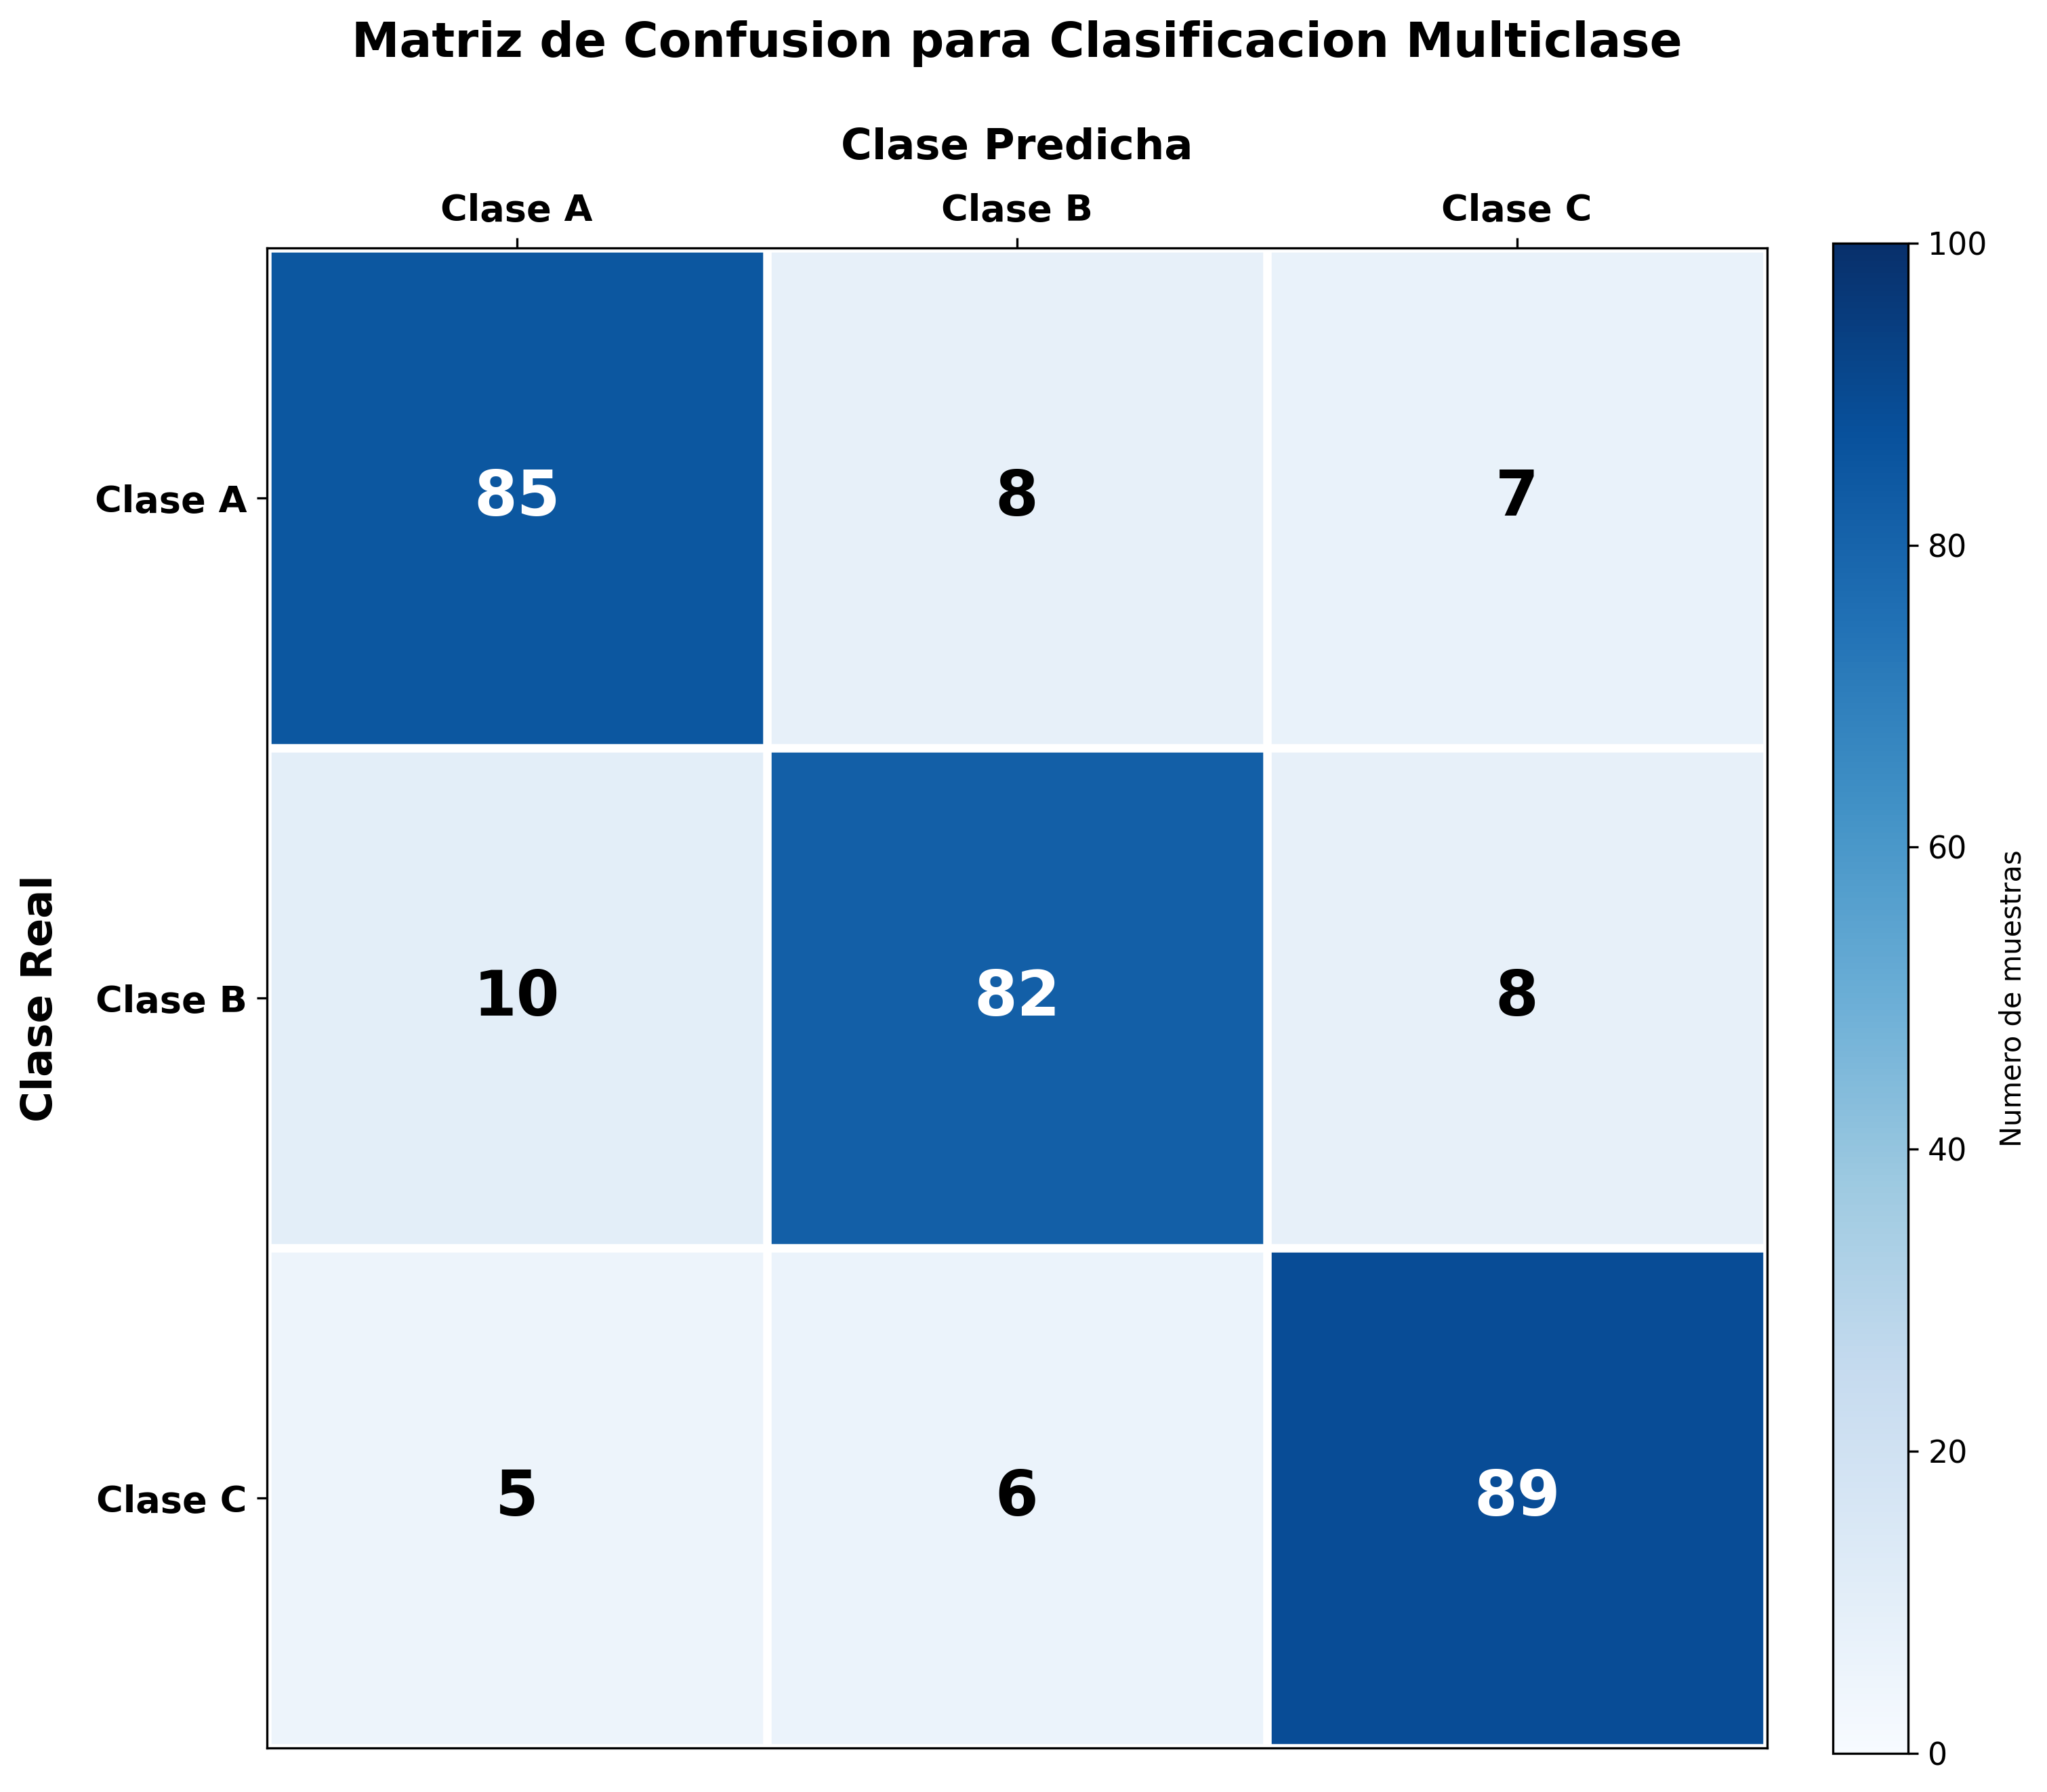
\includegraphics[width=0.65\textwidth]{imagenes/matriz_confusion_ejemplo.png}
\caption{\textit{Matriz de confusión para clasificación multiclase}}
\label{fig:matriz_confusion}
\end{table}

La precisión cuantifica la proporción de predicciones positivas correctas: $\text{Precision} = \text{TP}/(\text{TP} + \text{FP})$. La exhaustividad mide la proporción de casos positivos reales identificados: $\text{Recall} = \text{TP}/(\text{TP} + \text{FN})$. Existe un compromiso inherente entre precisión y recall: aumentar el umbral de decisión incrementa la precisión pero reduce el recall, y viceversa.

\subsubsection{Métricas para calibración espacial}

En sistemas de calibración píxel-milímetro, se emplean métricas de error continuo. El error cuadrático medio (RMSE) cuantifica la magnitud típica de los errores:

\begin{equation}
\text{RMSE} = \sqrt{\frac{1}{N}\sum_{i=1}^{N}(y_i - \hat{y}_i)^2}
\end{equation}

El coeficiente de determinación $R^2$ mide la proporción de varianza explicada por el modelo:

\begin{equation}
R^2 = 1 - \frac{\sum_{i=1}^{N}(y_i - \hat{y}_i)^2}{\sum_{i=1}^{N}(y_i - \bar{y})^2}
\end{equation}

Valores de $R^2$ cercanos a 1 indican excelente ajuste lineal del modelo. Para aplicaciones de agricultura de precisión, se requiere bajo RMSE (típicamente <2mm) y alto $R^2$ (>0.99) para garantizar precisión en el posicionamiento.


\section{Pruebas del Sistema Mecánico}
% Precision Posicionamiento


% Repetibilidad


% Velocidades Maximas


% Vibraciones Estabilidad



\section{Pruebas del Sistema de Control}
% Respuesta Temporal


\subsubsection{Manejo de errores y protecciones}

El firmware implementa mecanismos robustos de detección y manejo de errores para garantizar operación segura del sistema mecánico.

Antes de ejecutar cualquier comando, el analizador sintáctico valida sintaxis y rangos. Comandos inválidos retornan código de error inmediatamente sin ejecutar acción, previniendo movimientos peligrosos (Tabla \ref{tab:validacion_comandos}).

\begin{table}[H]
\centering
\small
\begin{tabular}{|l|l|l|}
\hline
Parámetro & Rango válido & Error \\
\hline
Delimitadores & \texttt{<} y \texttt{>} presentes & INVALID\_CMD \\
\hline
Velocidad H & 500 - 15,000 pasos/s & INVALID\_PARAM \\
\hline
Velocidad V & 500 - 12,000 pasos/s & INVALID\_PARAM \\
\hline
Ángulo servo & 10° - 160° & INVALID\_PARAM \\
\hline
Tiempo trayectoria & 0 - 10,000 ms & INVALID\_PARAM \\
\hline
\end{tabular}
\caption{\textit{Validaciones de comandos y rangos permitidos}}
\label{tab:validacion_comandos}
\end{table}

El firmware implementa supervisor de comunicación: si no recibe señal de sincronización (\texttt{HB:1}) del nivel superior durante un período prolongado, asume pérdida de comunicación y ejecuta detención de emergencia automática, deshabilitando todos los motores y entrando en modo seguro hasta recibir comando de reset.

El buffer UART circular (256 bytes) implementa protección contra overflow verificando espacio disponible antes de cada escritura. Si el buffer está lleno, el byte se descarta y se envía error de overflow. La Tabla \ref{tab:codigos_error} lista los códigos de error definidos.

\begin{table}[H]
\centering
\begin{tabular}{|l|p{9cm}|}
\hline
Código & Descripción y causa \\
\hline
INVALID\_CMD & Comando no reconocido o sintaxis incorrecta. \\
\hline
INVALID\_PARAM & Parámetros fuera de rango válido. \\
\hline
LIMIT\_HIT & Movimiento bloqueado por activación de final de carrera. \\
\hline
BUFFER\_OVERFLOW & Buffer UART saturado. \\
\hline
TIMEOUT & Operación excedió tiempo límite configurado. \\
\hline
SYSTEM\_ERROR & Error interno del firmware. \\
\hline
\end{tabular}
\caption{\textit{Códigos de error del firmware}}
\label{tab:codigos_error}
\end{table}

Los finales de carrera se monitorean continuamente. El sistema detecta la activación de cualquier límite y ejecuta inmediatamente la detención de emergencia: deshabilita los drivers (ENABLE = HIGH), detiene la generación de pulsos, envía notificación asíncrona al supervisor indicando el límite activado, y bloquea nuevos comandos de movimiento hacia el lado en el que se encuentra el fin de carrera. Esto previene daños mecánicos por intentos de movimiento en dirección bloqueada.

% Finales Carrera



\section{Pruebas del Sistema de IA}
% Precision Deteccion


% Tasa Clasificacion


% Tiempo Procesamiento


% Robustez Variaciones


% Validacion Mapeo



\section{Pruebas de Integración}
% Ciclo Completo


% Eficiencia Sistema


% Casos Extremos



\section{Análisis de Resultados}
% Comparacion Objetivos


% Limitaciones


% Mejoras Potenciales



%%%%%%%%%%%%%%%%%%%%%%%%%%%%%%%%%%%%%%%%%%%%%%%%%%%%%%%%%%%%%%%
% CAPÍTULO 5: CONCLUSIONES
%%%%%%%%%%%%%%%%%%%%%%%%%%%%%%%%%%%%%%%%%%%%%%%%%%%%%%%%%%%%%%%
\chapter{Conclusiones y Trabajo Futuro}

\section{Conclusiones Generales}
% Logros Alcanzados


El sistema cosechador automático de lechugas hidropónicas cumplió los objetivos planteados, validando la viabilidad técnica de automatización en agricultura vertical mediante integración de mecatrónica, visión artificial e inteligencia artificial.

\subsection*{Logros técnicos}

\textbf{Control jerárquico:} Arquitectura con separación funcional entre nivel regulatorio (control de actuadores en tiempo real) y supervisor (gestión de secuencias y coordinación con IA). Demostró ser robusta, escalable y modular.

\textbf{Visión e IA:} Métricas de desempeño: detección >90\%, clasificación de madurez 97\%, repetibilidad 88\%. Algoritmos basados en procesamiento morfológico y análisis estadístico de descriptores geométricos.

\textbf{Sistema mecánico:} Estructura cartesiana XZ + brazo serie 2 GDL. Precisión de posicionamiento 1\% en lazo abierto, tasa de agarres exitosos 82\% con realimentación visual.

\subsection*{Escalabilidad}

Software y algoritmos de IA son transferibles a escala industrial sin modificaciones estructurales. La arquitectura modular permite escalar mediante ajustes paramétricos (conversiones pasos/mm, límites, perfiles de velocidad).

\subsection*{Limitaciones identificadas}

\textbf{Rigidez estructural:} Material PETG del prototipo presenta flexibilidad excesiva generando vibraciones. Requiere transición a materiales de mayor módulo elástico.

\textbf{Iluminación:} Sistema funciona entre 800-1200 lux pero es sensible a variaciones. Requiere iluminación estabilizada o algoritmos adaptativos.

\subsection*{Viabilidad económica}

Costo de desarrollo: \$6.200.000 ARS. Período de recupero proyectado: 4 años (capacidad 55-60 lechugas/mes a \$2.500/unidad). Se requiere análisis detallado incluyendo costos operativos y escenarios de escalamiento.
% Lecciones Aprendidas



\section{Aportes del Proyecto}
% Innovaciones


% Contribuciones Tecnicas



\section{Trabajo Futuro}
% Mejoras Propuestas


% Escalabilidad


% Aplicaciones Potenciales



%%%%%%%%%%%%%%%%%%%%%%%%%%%%%%%%%%%%%%%%%%%%%%%%%%%%%%%%%%%%%%%
% ANEXOS
%%%%%%%%%%%%%%%%%%%%%%%%%%%%%%%%%%%%%%%%%%%%%%%%%%%%%%%%%%%%%%%
\appendix
\chapter{Diagramas Eléctricos Completos}
% A Diagramas Electricos



\chapter{Código Fuente Relevante}
% B Codigo Fuente



\chapter{Especificaciones Técnicas de Componentes}
% C Especificaciones



\chapter{Manual de Usuario}
% D Manual Usuario



\chapter{Hojas de Datos}
% E Hojas Datos



%%%%%%%%%%%%%%%%%%%%%%%%%%%%%%%%%%%%%%%%%%%%%%%%%%%%%%%%%%%%%%%
% REFERENCIAS
%%%%%%%%%%%%%%%%%%%%%%%%%%%%%%%%%%%%%%%%%%%%%%%%%%%%%%%%%%%%%%%
\chapter*{Referencias}
\addcontentsline{toc}{chapter}{Referencias}
% Referencias
% Referencias
\begin{enumerate}
    \item Módulo 04: Uniones Roscadas - Cátedra: Tenconología de contrucción y diseño mecánico - ng. Sebastián Lazo - Ing. Gabriel Mallon -ITU
\end{enumerate}


\end{document}